\documentclass[12pt,a4paper,oneside,openright]{book}
\usepackage[Italian]{babel}
\usepackage[T1]{fontenc}
\usepackage[utf8]{inputenc}
\usepackage{hyperref}
\usepackage{mathtools}
\usepackage{graphicx}
\usepackage{fancyhdr}
\newcommand{\fncyblank}{\fancyhf{}}
\newenvironment{abstract}%
{\cleardoublepage\fncyblank\null \vfill\begin{center}%
\bfseries \abstractname \end{center}}%
{\vfill\null}
\usepackage{float}
\renewcommand\labelenumi{(\theenumi)}
\begin{document}

\begin{abstract}
\begin{center}
Questo lavoro di tesi punta a migliorare le previsioni dei valori di dati multi-variati migliorando il trade-off tra accuratezza ed efficienza. 
\end{center}
\end{abstract}

\tableofcontents
\listoftables
\listoffigures

\chapter{Introduzione}
La rapida evoluzione, vissuta negli ultimi decenni, per la scienza e la tecnica ci porta oggi  a collezionare moli di dati impressionanti. È proprio in questi casi che soluzioni di analisi innovative che combinino informatica e statistica si rendono necessarie. 

In questi termini si presenta la problematica di dover effettuare previsioni accurate di ciò che sarà l’andamento futuro di un flusso di dati multi-variati e continuo nel tempo.

Al fine di risolvere tale problematica si utilizzano tecniche di data mining capaci di gestire tali flussi e di fornirne una rappresentazione funzionale all’applicazione di modelli di regressione che sono utili ad effettuare previsioni sull’andamento futuro dei dati in osservazione. 

In questo lavoro di tesi, partendo da un algoritmo che effettua previsione dopo aver applicato una tecnica di clustering incrementale e aver appreso un modello di regressione chiamato “Vector Autoregressive Model”, si investiga l’utilizzo della tecnica dello smoothing esponenziale e la costruzione di aggregati dei dati osservati in tempo reale, al fine di ottenere un bilanciamento tra accuratezza e efficienza nella costruzione di un modello di previsione multi-variato in reti di sensori.



In questo capitolo vengono descritti lo scenario applicativo all’interno del quale questo lavoro di tesi si colloca e si riporta una sintetica descrizione degli obiettivi prefissati. 
\newpage
\section{Scenario applicativo}
L’ormai diffuso uso delle reti di sensori ha portato a dover gestire sistemi informatizzati in grado di misurare e organizzare dati multi-variati in tempo reale. Tali sistemi si avvalgono dei cosiddetti geosensori, ovvero di dispositivi in grado di eseguire rilevazioni temporali multiple di fenomeni fisici quali per esempio temperatura, umidità, velocità del vento e livello delle radiazioni solari. 


Il fine ultimo di tali rilevazioni è senza dubbio quello di dover effettuare previsioni accurate di ciò che potrà essere l’andamento futuro di tali fenomeni, ma utilizzare queste informazioni non è semplice, non perché sia complicato leggerle, ma piuttosto perché è difficile interpretarle. 


È in questo contesto che l’algoritmo VARForecaster trova spazio, infatti utilizza una tecnica che ci aiuta a raffinare le informazioni derivanti dai geosensori proveniente dall’insieme di tecniche e metodologie definito data mining e che si chiama analisi dei cluster. L’utilizzazione di questa tecnica ci permette di raggruppare i geosensori in base alla loro vicinanza spaziale e alla similarità delle loro osservazioni.

Per ognuno di questi gruppi distinti, si possono costruire modelli di regressione, ovvero è possibile definire un modello secondo il quale “una variabile dipendente è modellata come una funzione delle variabili indipendenti più un termine d'errore” \cite{2a}.

A causa della natura delle rilevazioni, per avere delle previsioni valide e accurate è necessario che esse siano ripetute nel tempo, portando infine ad avere una serie temporale multi-variata (che considera più di un fenomeno) e georeferenziata (cioè geograficamente distribuita).


La previsione in un serie temporale multi-variata è realizzata con l'apprendimento di un modello VAR che restituisce un modello di regressione per ciascuna variabile. Tale modello di regressione predice i valori attesi per la variabile dipendente in funzione delle osservazioni storiche collezionate tanto per la variabile dipendente, cioè da predire, quanto per le variabili indipendenti, ovvero quelle rimanenti nel sistema di variabili misurate \cite{3a}. L'apprendimento di un modello VAR per sensore è computazionalmente costoso. La alternativa è l'apprendimento di un modello VAR per gruppi cluster di sensori.


In \cite{donato} si presenta un algoritmo, VARForecaster che combina modello di clustering e modello VAR. Il clustering è realizzato in maniera incrementale sulla base di approssimazioni dei valori osservati, ovvero si forma incrementalmente una gerarchia di cluster, partendo da un nodo radice inizialmente vuoto e aggiungendo istanze una alla volta aggiornando l’albero appropriatamente ad ogni passaggio, anche se questo comporta la ristrutturazione dell’albero \cite{4a}.

In questo lavoro di tesi si presenta una variante di tale algoritmo che: (1) valuta l'uso del meccanismo di smoothing esponenziale per determinare il modello di clustering sulla base dei valori geofisici attesi nella rete all'istante t+1 piuttosto che sulla base dei valori geofisici osservati all'istante t; (2) calcola aggregati dei dati in tempo reale (media o mediana) piuttosto che ricorrere ad approssimazioni degli stessi. Lo scopo è identificare la soluzione che realizza il miglior bilanciamento tra accuratezza e efficienza.
\newpage
\section{Obiettivi e contributi}
Questo lavoro di tesi considera un algoritmo incrementale di clustering spazio-temporale multi-variato e lo estende nelle seguenti direzioni: 
\begin{itemize}
\item definizione, nell’albero binario rappresentante il clustering, di un nuovo criterio di ricalcolo della media dei nodi creati ex-novo in fase di riapprendimento (in \cite{donato} si era definito un calcolo basato sulla media del padre per ognuno di essi);
\item utilizzo, per il riapprendimento dell’albero suddetto, dell’algoritmo di smoothing esponenziale, al fine di fornire un mezzo più efficace per la previsione dei valori futuri della serie di dati (in \cite{donato} tale albero era appreso solo in base ai valori ricevuti dai sensori, presenti all’interno della finestra temporale di ogni nodo).
\end{itemize}
\chapter{Stato dell'arte}
\section{Smoothing}
Come definito in precedenza, a causa della natura delle rilevazioni, al fine di migliorare l'accuratezza delle previsioni è indispensabile che queste siano ripetute nel tempo, e che quindi sia fornita una serie temporale di esse.

In questo lavoro di tesi si considera il caso in cui la serie temporale è multi-variata, ovvero prende in considerazione più variabili, e geo-referenziata, cioè i valori sono rilevati da sensori geograficamente distribuiti.

Una serie temporale, quindi, altro non è che una sequenza di osservazioni le quali sono state ripetute nel tempo. 

In una serie temporale, così come in una qualsiasi collezione di dati temporalmente distribuita, i valori assunti dalle variabili hanno una certa variazione random. 

Esistono delle tecniche per ridurre gli effetti dovuti a tali variazioni, e che se utilizzate appropriatamente, rivelano con più chiarezza i pattern nascosti presenti tra i dati. Queste sono dette tecniche di "smoothing" \cite{5a}. 

Lo smoothing è un processo che viene usato per la previsione di valori futuri in una serie temporale e, in statistica e nel campo dell'elaborazione digitale delle immagini, per evidenziare i pattern significativi presenti all'interno dei dati, attenuando il rumore generato da artefatti ambientali, informatici o elettronici. 

Nella pratica esso è un processo in cui i valori presenti in un dataset sono mediati con i loro vicini spaziali o temporali in una serie, tipo una serie temporale, o un'immagine \cite{6a}. 

Ci sono diversi tipi di smoothing:
\begin{itemize}
\item Media mobile semplice: per la previsione vengono considerate tutte le osservazioni precedenti, alle quali viene dato lo stesso peso, indipendentemente dall'istante temporale in cui ci troviamo. La relativa formula per il calcolo è la seguente

\begin{center}
$Y_{t+1}$ = $Y_{t}$+$Y_{t-1}$+$Y_{t-2}$+ ... + $Y_{t-n+1}$ n
\end{center}

\item Media mobile ponderata: è una variante dello smoothing a virgola mobile ed in questo caso i valori precedenti non hanno tutti lo stesso peso, bensì viene assegnato ad ognuno di essi un fattore, chiamato peso, che varierà l'influenza di tale termine all'interno della sommatoria. La formula è così definita

\begin{center}
$Y_{t+1}$ = $p_{1}$ $Y_{t}$+ $p_{2}$ $Y_{t-1}$+ $p_{3}$ $Y_{t-2}$+ ... + $p_{n}$ $Y_{t-n+1}$
\end{center}

dove 
$p_{{i}}$ > {0} e $\sum_{i=1}^{i={n}}{ p_{{i}}} = {1}$


\item Esponenziale.
\end{itemize}

Nella seguente sezione è descritto lo smoothing esponenziale nel dettaglio.
\newpage
\subsection{Exponential Smoothing}
Lo smoothing esponenziale nacque alla fine degli anni '50 (i pionieri furono Holt nel 1957, Brown nel 1959 e Winters nel 1960) e motivò alcuni dei metodi di previsione (forecast) di maggior successo. Le previsioni ottenute con i metodi di smoothing esponenziale sono medie ponderate delle osservazioni passate, con i pesi che diminuiscono in modo esponenziale con l'andare avanti delle osservazioni. 

In altri termini, le osservazioni più recenti hanno un peso associato più alto. 

Questo modo di operare genera previsioni accurate in modo più veloce e per un ampio spettro di serie temporali, il che è un grande vantaggio per le applicazioni in campo industriale \cite{7a}.

Essendo l'idea di base quella di "pesare" maggiormente le osservazioni più recenti rispetto a quelle più remote nel passato, i metodi di smoothing sono capaci di adeguarsi rapidamente a variazioni improvvise nel valore della serie storica a causa di eventi che modificano la regolarità del fenomeno osservato, come per es. può essere un giorno con elevata umidità oppure particolarmente ventoso. 

Esistono diversi metodi di smoothing esponenziale, che tengono conto o meno dell'esistenza di componenti tendenziali e stagionali nella serie storica in esame e sono:
\begin{itemize}
\item Metodo di Brown;
\item Metodo di Holt;
\item Metodo di Winters.
\end{itemize}

\subsubsection{Metodo di Brown}
Il {\bfseries metodo di Brown} è il più semplice e la sua formula è la seguente:
\begin{center}
$Y_{t}$ = $\alpha$ $x_{t}$ + (${1 - \alpha }$) $Y_{t-1}$
\end{center}

dove $\alpha$ è il fattore di smoothing, con 0 $\leq$ $\alpha$  $\leq$ 1. In altre parole $Y_{t}$ è la media pesata dell'osservazione corrente $x_{t}$ ed il precedente termine a cui era stato applicato lo smoothing $Y_{t-1}$. Il fattore di smoothing è il termine, all'interno dell'equazione, che indica quanto peso dare al fattore precedente o all'osservazione corrente. 

Infatti se $\alpha$ = 1 la serie in uscita allo smoothing è sempre quella ricevuta in ingresso, mentre man mano che si abbassa il valore di questo fattore si ha minor adattamento ai dati correnti fino a quando, con $\alpha$ = 0, si avrà in output sempre la serie di partenza.

In questo metodo il valore $Y_{1}$ è uguale al valore della prima osservazione effettuata $x_{1}$.

Questo tipo di smoothing esponenziale è molto facile da applicare, infatti basta che due osservazioni siano disponibili per poterlo utilizzare e non tiene conto ne di eventuali trend né di stagionalità all'interno della serie temporale.
\subsubsection{Metodo di Holt}
Il {\bfseries metodo di Holt} migliora il modello di Brown, infatti tiene conto dei trend presenti all'interno della serie temporale (ma non della stagionalità). La formula per calcolare la previsione con il suddetto metodo è la seguente:

 \begin{center} 
$Y_{t+1}$ = $Y_{t}$ + $m_{t}$  
\end{center} 
\begin{flushright}
(1)
\end{flushright}

dove: 
\begin{itemize}

\item $Y_{t}$ = $\alpha$ $x_{t}$ + (${1 - \alpha }$)($Y_{t-1}$ + $m_{t-1}$) $\forall$ $t$ $\geq$ 2 
\begin{flushright}
(2)
\end{flushright}
\item $m_{t}$ = $\beta$ ($Y_{t}$ - $Y_{t-1}$)+(1 - $\beta$) $m_{t-1}$ $\forall$ $t$ $\geq$ 2 
\begin{flushright}
(3)
\end{flushright}
\item $Y_{1}$ = $x_{1}$

\item $m_{1}$ = $x_{2}$ - $x_{1}$
\end{itemize}


L'equazione (1) è definita equazione di predizione, la (2) equazione di livello e la (3) come equazione di trend. 

$Y_{t}$ denota lo stimatore della serie temporale all'istante $t$, $m_{t}$ è uno stimatore del trend della serie all'istante $t$, $\alpha$ è, come nel modello di Brown, il parametro di smoothing per la serie e può essere 0 $\leq$ $\alpha$ $\leq$ 1 e $\beta$ invece è il parametro di smoothing per il trend e può anch'esso assumere valori 0 $\leq$ $\beta$ $\leq$ 1. 
$\beta$ deve essere ottimizzato minimizzando lo scarto quadratico medio.

\subsubsection{Metodo di Winters}

Il {\bfseries metodo di Winters}, infine, è il metodo di smoothing esponenziale con più alta complessità ma che si preoccupa di tenere in considerazione, oltre che dei trend presenti all'interno della serie temporale, anche di una stagionalità di periodo L nota. Esso si calcola come segue:

\begin{center}
$Y_{t+1}$ = ($Y_{t}$ + $m_{t}$) $q_{t-L+1}$
\end{center}
\begin{flushright}
(1)
\end{flushright}
dove:
\medskip \medskip
\begin{itemize}

\item $Y_{t}$ = $\alpha$ $\frac{Y_{t}}{q_{t-L} }$ + (1 - $\alpha$)($Y_{t-1}$ + $m_{t-1}$) $\forall$ $t$ $\geq$ 2 
\begin{flushright}
(2)
\end{flushright}
\item $m_{t}$ = $\beta$ ($Y_{t}$ - $Y_{t-1}$) + (1- $\beta$)$m_{t-1}$   $\forall$ $t$ $\geq$ 2
\begin{flushright}
(3)
\end{flushright}
\item $q_{t}$ = $\gamma$ $\frac{x_{t}}{Y_{t}}$ + (1 - $\gamma$) $q_{t-L}$  $\forall$ $t$ $\geq$ L + 1 
\begin{flushright}
(4)
\end{flushright}
\item $q_{t}$ = $\frac{x_{t}}{\sum_{\tau=1}^{L}{\frac{x_{\tau}}{L}}}$ $\forall$ $t$ = 1, $\dots$ , L
\begin{flushright}
(5)
\end{flushright}

\item $Y_{1}$ = $x_{1}$

\item $m_{1}$ = $x_{2}$ - $x_{1}$
\end{itemize}

L'equazione (1) è definita equazione di predizione, la (2) equazione di livello, la (3) equazione di trend, mentre la (4) e la (5) sono chiamate equazioni di periodo.

$Y_{t}$ denota lo stimatore della serie temporale all'istante $t$, $m_{t}$ è uno stimatore del trend della serie all'istante $t$ e $q_{t}$ indica uno stimatore della periodicità della serie all'istante $t$, il quale deve essere calcolato in due modi diversi che dipendono dall'istante temporale in cui ci si trova rispetto all'intera durata del periodo.

$\alpha$ è il parametro di smoothing per la serie e può essere 0 $\leq$ $\alpha$ $\leq$ 1, allo stesso modo $\beta$, che è il parametro di smoothing del trend della serie temporale, deve essere 0 $\leq$ $\beta$ $\leq$ 1, invece $\gamma$ è il parametro di smoothing del periodo e può essere 0 $\leq$ $\gamma$ $\leq$ 1. 

$\gamma$ deve essere ottimizzato minimizzando lo scarto quadratico medio.

\medskip \medskip

È possibile, nel caso lo si desideri, eliminare da una serie temporale la componente di tendenza o di stagionalità.
Innanzitutto bisogna determinare la tendenza con un'analisi di regressione e la componente di stagionalità tramite scomposizione della serie, successivamente è possibile calcolare la media mobile per rimuovere la tendenza e, per differenziazioni successive ($B_{t}$($h$) = $y_{t}$ - $y_{t-h}$), è possibile rimuovere la tendenza \cite{8a}.

\newpage
\section{Vector Autoregressive Model}
Il modello VAR (Vector Autoregressive Model) è uno dei modelli  più flessibili, facili da usare e di successo per l'analisi di serie temporali multivariate. E' un'estensione naturale del modello autoregressivo univariato verso il dinamismo delle serie temporali multivariate. Il modello VAR ha dimostrato di essere molto utile per descrivere il comportamento dinamico delle serie storiche economiche e finanziarie e per le previsioni. Esso fornisce previsioni spesso più accurate rispetto a quelle dei modelli univariati, infatti queste possono essere condizionate da potenziali percorsi futuri che le variabili nel modello possono prendere. Oltre alla descrizione dei dati e la previsione, il modello VAR può essere usato per l'inferenza struttura e per l'analisi della linea di condotta \cite{13a}. 

L'analisi del modello VAR può essere affrontata da due punti di vista: 
\begin{itemize}
\item dal punto di vista teorico: è in questa sezione descritta la storia di tale modello e la teoricità sulla quale è basato;
\item dal punto di vista implementativo: è invece qui descritta la tecnica di utilizzazione del modello VAR in base alle necessità di questo progetto di tesi.
\end{itemize}
\newpage 
\subsection{Modelli teorici}
I modelli VAR sono stati definiti da Christopher Sims in uno storico articolo pubblicato su Econometria nel 1980, che proponeva una critica dei modelli strutturali di equazioni simultanee, allora il principale strumento di analisi ecometrica nell'ambito della macroeconomia. 

In particolare, i modelli VAR risultano nel complesso più semplici rispetto ai modelli strutturali, e la loro performance in termini di capacità previsiva di variabili macroeconomiche appare migliore.

Tutte le n variabili date in input al modello, vengono trattate simmetricamente in senso strutturale dove ognuna di essa sarà ricavata da un’equazione che spiega la sua evoluzione in base ai ritardi di se stessa e ai ritardi di tutte le altre variabili. 

Le variabili che vengono date in input al modello VAR, prendono il nome di variabili endogene e vengono raccolte in un vettore $Y_{t}$ di dimensione n x 1 che ha come i-esimo elemento $Y_{it}$ e dove quest’ultimo rappresenta l’osservazione della variabile i-esima al tempo t. Ad esempio se la variabile i-esima è la velocità del vento, allora $Y_{it}$ è il valore della velocità del vento al tempo t \cite{9a} \cite {10a}. 

Un modello VAR, in generale, è un sistema di equazioni simultanee che può essere descritto mediante tre modelli teorici: reduced form (o forma ridotta), structural form (o forma strutturale) e companion form.  
\subsubsection{Reduced form}
Il modello VAR in forma ridotta si presenta nella forma:
\begin{center}
{\bfseries  $Y_{t}$ = c + $\Phi$(L)$Y_{t-1}$ + $\varepsilon_{t}$ = c + $\Phi_{1}$ $T_{t-1}$ + $\dots$ + $\Phi_{p}$ $Y_{t-p}$ + $\varepsilon_{t}$ }
\end{center}

dove, per un  VAR(p) {\bfseries  $\Phi$(L) = $\sum_{i=0}^{p-1}{\Phi_{i} L^{i}}$} è un polinomio matriciale di ordine p nell'operatore di ritardo {\bfseries L} (ossia, l'operatore tale che {\bfseries $L^{i}$ $Y_{t}$ = $Y_{t-1}$}), con {\bfseries $\Phi_{i}$} che è una matrice di dimensione n x n; 

{\bfseries $Y_{t}$} è il vettore delle variabili endogene e si presenta nella forma:
\begin{center}
{\bfseries $Y_{t}$ = $\begin{bmatrix}
Y_{1t}\\ \vdots \\ Y_{nt} 
\end{bmatrix}$ }
\end{center}
e $\varepsilon_{t}$ è un vettore conforme di disturbi stocastici del tipo:
\begin{center}
{\bfseries $\varepsilon_{t}$ = $\begin{bmatrix}
\varepsilon_{1t}\\ \vdots \\ \varepsilon_{nt} 
\end{bmatrix}$ }
\end{center}
tali che {\bfseries $E_{\varepsilon_{t}}$ = 0} (ogni termine di disturbo ha media pari a zero) e {\bfseries E($\varepsilon^2_{it}$) = $\sigma^2_{i}$} con {\bfseries i = 1, \dots, n} dove {\bfseries $\sigma^2_{i}$} è la varianza i-esima ed E la media. Si osservi che gli elementi del vettore $\varepsilon_{t}$ non sono necessariamente non correlati, cioè che in generale {\bfseries E($\varepsilon_{it}$ $\varepsilon_{jt}$) = $\sigma_{ij}$ $\neq$ 0 } (la deviazione standard fra due elementi di $\varepsilon_{t}$ può essere diversa da zero) per elementi di $\varepsilon$ indicizzati da {\bfseries i, j}  con {\bfseries j $\neq$ i}; per contro, per ipotesi nessuna delle componenti del vettore $\varepsilon$ esibisce correlazione seriale, ossia {\bfseries E($\varepsilon_{it}$ $\varepsilon_{i \tau}$) = 0, $\forall{i}$ e $\forall{\tau}$ $\neq$ t}.

Infine, resta da indicare il vettore {\bfseries c}, ossia il vettore delle costanti (o intercetta) che si presenta nella seguente forma: 
\begin{center}
{\bfseries c = 
$\begin{bmatrix}
c_{1} \\ \vdots \\ c_{n}
\end{bmatrix}$  }
\end{center}

Per capire ancora meglio la reduced form, consideriamo il modello VAR dal punto di vista della stima dei coefficienti, in modo tale da poterlo scrivere anche nel seguente modo: 
\begin{center}
{\bfseries
$y_{1t}$ = $c_{1}$ + $\varphi^{(1)}_{11}$ $y_{1t-1}$ + $\dots$ + $\varphi^{(p)}_{1p}$ $y_{nt-p}$ + $\varepsilon_{1t}$ 

$\vdots$

$y_{nt}$ = $c_n$+ $\varphi_{n1}^{(1)}y_{1t-1}$+$\dots$+$\varphi_{np}^{(p)}y_{nt-p}$+$\varepsilon_{nt}$
}
\end{center}

Osservando che al secondo membro di ogni equazione figurano le stesse variabili, il VAR(p) risulta equivalente ad un modello SURE (Seemingly Unrelated Regression Equations), i cui coefficienti possono essere stimati considerando ogni equazione come una regressione lineare standard, indipendente dalle altre. In particolare, gli stimatori OLS (Ordinary Least Squares) ottenuti con il metodo dei minimi quadrati, risultano consistenti e cioè che all'aumentare dell'informazione, la distribuzione di probabilità di ognuna di esso, si concentra in corrispondenza del valore del parametro da stimare \cite{11a}.
\subsubsection{Structural form}
La structural form di un modello VAR(p) è formalizzata da un'equazione del tipo:
\begin{center}
{\bfseries 
$A_o$ $Y_t$ = m + $A$ (L) $Y_{t-1}$ + $u_t$
}
\end{center}
dove {\bfseries m} è simile al vettore di costanti {\bfseries c} della reduced form, {\bfseries $A_0$} è la matrice n x n che identifica le relazioni strutturali contemporanee tra le diverse componenti di {\bfseries $Y_t$}, mentre il vettore {\bfseries $u_t$} è chiamato rumore bianco ed è un vettore di disturbi che in particolare ha componenti tra loro correlate: {\bfseries E($u_{it}$ $u_{ij}$) = 0} per {\bfseries j $\neq$ i}.

Come si può notare, la forma strutturale è molto simile a quella ridotta con la differenza di avere la matrice $A_0$ al primo membro: all'interno di essa, e precisamente, sulla sua diagonale principale, si avranno elementi tutti pari a 1 e quindi vuol dire che il valore 1 lo si avrà alla variabile i-esima in corrispondenza dell'equazione i-esima. 

La structural form è una forma di supporto per la reduced form, e questo perché possiamo passare dalla prima forma alla seconda pre-moltiplicando a sinistra di ambo i membri l'inversa della matrice $A_0$:
\begin{center}
{\bfseries
$\mathbf{Y}_t$=$A_0^{-1}$ $\mathbf{m}$+$A_0^{-1}$ $A(L)$ $\mathbf{Y}_{t-1}$+$A_0^{-1}u_t$=$\mathbf{c}$+$\Phi(L)$ $\mathbf{Y}_{t-1}$+$\varepsilon$
}
\end{center}

Quest'ultima la si può riscrivere in questo modo:
\begin{center}
{\bfseries
$\left(I-\Phi(L)L\right)$ $\mathbf{Y}_t$=$\mathbf{c}$+$A_0^{-1}$ $u_t$
}
\end{center}

da cui si ottiene una forma detta forma finale del modello VAR(p) o rappresentazione di Wold:
\begin{center}
{\bfseries
$\mathbf{Y}_t$=$\left(I-\Phi(L)L\right)^{-1}\mathbf{c}+\left(I-\Phi(L)L\right)^{-1}$ $A_0^{-1}$ $u_t$=$\mathbf{\mu}$+$\Psi$(L)$u_t$
}
\end{center}

dove {\bfseries I} è la matrice identica, {\bfseries $\Psi$ (L)} è un polinomio matriciale nell'operatore L di ordine finito, e {\bfseries $\mu$} è il valore atteso non condizionato di {\bfseries $Y_t$}. In altre parole, il VAR(p), processo vettoriale autoregressivo di ordine finito, è equivalente a un processo in media mobile di ordine infinito.
\subsubsection{Companion form}
La companion form di un modello VAR(p) è la riscrittura della sua reduced form con l'accorpamento di p espressioni vettoriali. L'equazione rappresentante questa nuova forma è la seguente:
\begin{center}
{\bfseries
$\begin{bmatrix}\mathbf{Y}_t\\\mathbf{Y}_{t-1}\\\vdots\\\mathbf{Y}_{t-p+1}\\\end{bmatrix}$=$\begin{bmatrix}\mathbf{c}\\\mathbf{0}\\\vdots\\\mathbf{0}\end{bmatrix}$+$\begin{bmatrix}\Phi_1 & \Phi_2 & \cdots & \Phi_{p-1} & \Phi_p\\ I & \mathbf{0} & \cdots & \mathbf{0} & \mathbf{0}\\ \mathbf{0} & I & \cdots & \mathbf{0} & \mathbf{0}\\ \vdots & \vdots & \ddots & \vdots & \vdots\\ \mathbf{0} & \mathbf{0} & \cdots & I & \mathbf{0}\end{bmatrix}$ $\begin{bmatrix}\mathbf{Y}_{t-1}\\\mathbf{Y}_{t-2}\\\vdots\\\mathbf{Y}_{t-p}\\\end{bmatrix}$ + $\begin{bmatrix}A_0^{-1}u_t\\ \mathbf{0}\\ \vdots\\ \mathbf{0}\end{bmatrix}$
}
\end{center}

Seguendo la notazione prima descritta, si possono identificare, in questa equazione, quattro vettori di vettori e una matrice di matrici, dove gli zeri presenti nei vettori e nella matrice rappresentano rispettivamente vettori nulli di dimensione n x 1 e matrici nulle di dimensioni n x n. 

È possibile riscrivere l'equazione nel seguente modo: 
\begin{center}
{\bfseries
$Z_t$ = $\lambda$ + $F$|$Z_{t-1}$ + $\xi_t$
}
\end{center}
dove E($\xi_t$) = 0, ed essendo $\xi_t$ = [$\xi^{'}_1$, $\dots$, $\xi^{'}_T$]', si ha E($\xi$ $\xi^{'}$) = $\sum$ $\otimes$ $I_t$ dove $\sum$ è la matrice varianze-covarianze dei disturbi $\varepsilon$ e $\otimes$ indica il prodotto di Kroenecker.
\medskip

È importante sottolineare, infine, che la forma adottata generalmente da un modello VAR per effettuare analisi statistiche dei dati, è la {\bfseries reduced form}.
\newpage
\subsection{Implementazione in R}
R è un linguaggio e un ambiente di sviluppo per l'analisi statistica e grafica.

È un progetto GNU simile al linguaggio e ambiente di sviluppo S, il quale fu sviluppato ai laboratori Bell (Bell Laboratories) da John Chambers e i suoi colleghi. R può essere considerato come una diversa implementazione di S. Ci sono importanti differenze, ma molto del codice scritto in S può essere eseguito senza dover apporre modifiche in R. 

R fornisce un'ampia varietà di tecniche statistiche (modellazione lineare e non, test statistici classici, analisi di serie temporali, classificazione, clustering, $\dots$) e grafiche ed è molto estendibile. 

Le sue caratteristiche principali sono:
\begin{itemize}
\item semplicità nella gestione e manipolazione dei dati;
\item disponibilità di una suite di strumenti per calcoli su vettori, matrici, ed altre operazioni complesse;
\item accesso ad un vasto insieme integrati per l'analisi statistica;
\item produzione di numerose potenzialità grafiche particolarmente flessibili;
\item possibilità di adoperare un vero e proprio linguaggio di programmazione orientato ad oggetti che consente l'uso di strutture condizionali e cicliche, nonché di funzioni create dall'utente;
\end{itemize}
È distribuito gratuitamente sotto i vincoli GPL (General Public License) ed è disponibile per diverse architetture hardware e sistemi operativi: Unix, Linux, Windows, MacOS. Sul sito della  CRAN (\url{<http:\\www.r-project.org)>} è possibile scaricare, oltre che il programma base, anche una serie di moduli aggiuntivi e un'ampia manualistica sull'ambiente, che va dall'installazione del software al suo utilizzo all'analisi dei dati \cite{12a}.

Sono di seguito descritte le due funzioni in R considerate nella realizzazione di questo progetto di tesi:
\begin{itemize}
\item VARselect;
\item VAR;
\end{itemize}
\newpage
\subsubsection{VARSelect}
\begin{center}
{\bfseries 
VARselect(y, lag.max = value1, type = value2, season = value3, exogen = value4)
}
\end{center}
dove:
\begin{itemize}
\item y è la matrice delle variabili endogene (cap. 2.1);
\item lag.max, ossia il valore value1, è il massimo ordine di ritardo che si potrà avere nel modello VAR;
\item type, nonché value2, rappresenta il tipo di regressori deterministici da includere nel modello VAR e uno dei possibili valori che può essere assegnato è: "const" (costante), "trend" (tendenza), "both" (entrambi, cioè costante e tendenza) e "none" (nessuno);
\item season è la frequenza stagionale (periodicità) dei dati. Se value3 = 4 vorrebbe dire che si avranno dei dati trimestrali. Può assumere valore "NULL" e in questo caso indicherebbe un'assenza di stagionalità;
\item exogen, ovvero value 4, rappresenta la matrice delle variabili esogene, cioè delle variabili indipendenti. Può assumere valore "NULL" e sta ad indicare che non ci sono variabili esogene.
\end{itemize}

Gli output sono:
\begin{itemize}
\item selection. È il vettore degli ordini ottimali ottenuti ognuno da ogni criterio possibile. I criteri sono delle funzioni avente un solo input e i criteri possibili sono quattro;
\item criteria. È la matrice di dimensione 4 x lag.max contenente i valori ottenuti da ogni criterio attribuendo input che vanno da 1 fino a lag.max.
\end{itemize}
\newpage
È di seguito riportato un esempio d'uso di questa funzione, con l'utilizzo del dataset "Canada" predefinito in R \cite{20a}.

Questo dataset riporta le rilevazioni ottenute su quattro attributi effettuate trimestralmente dal 1980 al 2000. Tali attributi sono: 
\begin{itemize}
\item e
\item prod
\item rw
\item U
\end{itemize}

\begin{figure}[H]
\textbf{
\centering
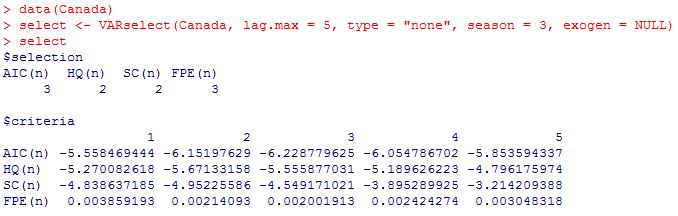
\includegraphics[width=\textwidth]{VAR/select.jpg}
\caption{Esempio di utilizzo della funzione VARSelect}
\label{VARSelect}
}
\end{figure}
\newpage
\subsubsection{VAR}
\begin{center}
{\bfseries 
VAR(y, p = value1, type = value2, season = value3, exogen = value4, lag.max = value5, ic = value6)
}
\end{center}

dove i parametri già specificati per la funzione VARselect valgono anche qui mentre:
\begin{itemize}
\item p, nonché value1, rappresenta l'ordine di ritardo scelto per il modello VAR;
\item ic, cioè value6, è l'informazione sul criterio utilizzato. I possibili criteri sono: "AIC" (Akaike), "HQ" (Hannan-Quinn), "SC" (Schwarz), "FPE" (Forecast Predict Error).
\end{itemize}
Gli output invece sono:
\begin{itemize}
\item p. È l'ordine di ritardo dato in input;
\item K. Rappresenta la dimensione del modello VAR (cioè è il numero di attributi della matrice y data in input alla funzione VAR);
\item varresult. È la lista di oggetti di regressione, dove ogni oggetto sarà associato al rispettivo attributo della matrice y data in input alla funzione VAR. Ad ognuno di questi oggetti è associato un vettore di coefficienti stimati tramite la regressione che si chiama coefficients. Questo vettore avrà un numero di coefficienti pari a p x K \cite{13a}.
\end{itemize}

Come esempio di utilizzo di questa funzione si mostra la continuazione dell'apprendimento del modello VAR sul dataset Canada. 
\begin{figure}[H]
\textbf{
\centering
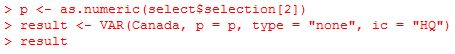
\includegraphics[width=\textwidth]{VAR/fVAR.jpg}
\caption{Esempio di utilizzo della funzione VAR}
\label{fVAR}
}
\end{figure}
In fig.~\ref{fVAR}, dalla posizione scelta all'interno del vettore in output dalla funzione \textit{"VARselect"}, \textit{"selection"}, per la lettura di p, è possibile notare come il criterio utilizzato sia \textit{"HQ"}.

Inoltre è ben visibile l'utilizzo di soli quattro parametri per il corretto utilizzo della funzione VAR, e ciò è possibile perché in precedenza è stata utilizzata la funzione \textit{VARselect} per la determinazione degli ordini di ritardo ottimali per ogni criterio.
\begin{figure}[H]
\textbf{
\centering
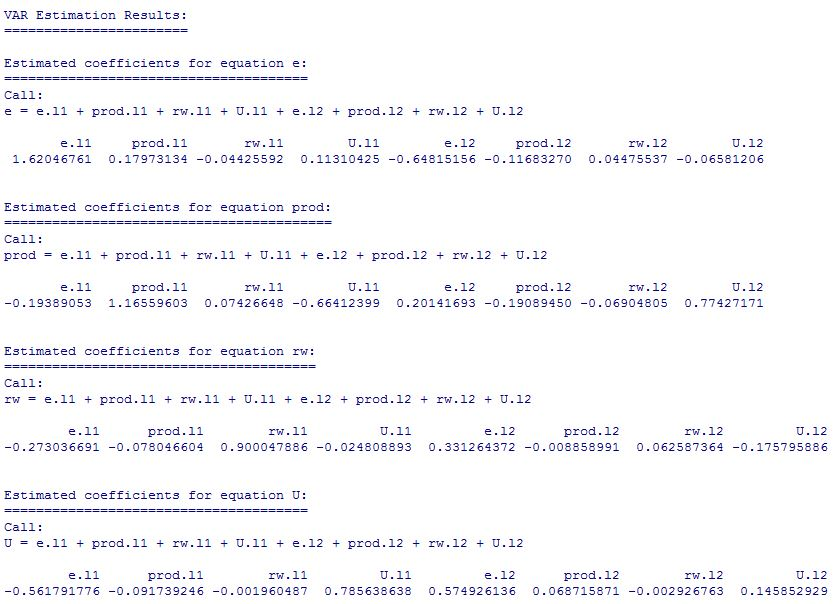
\includegraphics[width=\textwidth]{VAR/fVARo.jpg}
\caption{Output della funzione in fig.~\ref{fVAR}}
\label{fVARo}
}
\end{figure}

In fig.~\ref{fVARo} è possibile notare che il modello VAR appreso combina i valori presenti all'interno del dataset con una serie di coefficienti in modo tale da costruire una combinazione lineare necessaria per il calcolo dei valori futuri di ogni attributo. Si specifica che la struttura di ogni addendo all'interno delle equazioni è definita come:
\begin{itemize}
\item nome dell'attributo;
\item .l;
\item la quantità di istanti temporali di cui bisogna spostarsi indietro per recuperare il valore da moltiplicare con il rispettivo coefficiente.
\end{itemize}

Si noti inoltre che ogni attributo è messo in relazione con tutti gli altri (anche con se stesso) e che il modello si sposta di due elementi indietro nella finestra temporale. Tale valore è determinato dall'ordine di ritardo ottimale per il criterio scelto (che ricordiamo essere due).
\newpage
\section{Clustering}
Il \textit{clustering} è una tecnica di apprendimento non supervisionato la quale organizza un'insieme di istanze in gruppi di similarità. 

Tali gruppi, che contengono al loro interno istanze simili tra loro ma dissimili con le istanze contenute negli altri gruppi, vengono definiti \textit{\textbf{cluster}}. 

Le istanze all'interno di un gruppo sono chiamate \textit{oggetti} o \textit{data point} e l'istanza centrale del cluster è definito \textit{centroide}.

L'obiettivo di un clustering è quindi quello di scoprire il raggruppamento dei dati attraverso l'uso di un algoritmo di clustering e di una funzione che calcola la similarità (/dissimilarità) tra essi \cite{16a}.

Sono di seguito descritti le principali tecniche di clustering:
\begin{itemize}
\item Clustering partizionale;
\item Clustering gerarchico;
\item Cluster concettuale e interpolativo.
\end{itemize}

\subsection{Clustering partizionale}
Il clustering partizionale è una tecnica di clustering che punta a suddividere le istanze di un dataset in \textit{k} cluster. Tale numero è a discrezione dell'utente e può essere $1$ $\leq$ k $\leq$ $|n|$ con |n| cardinalità massima dell'insieme delle istanze \cite{17a}. 

L'algoritmo più utilizzato in letteratura che implementa questa tecnica è il k-means.

Il passo base della procedura prevede la costruzione di k cluster, ognuno contenente un solo oggetto, scelto in base ad alcuni criteri. Esso è il textit{centroide} del cluster e ne è rappresentativo. Per definire a quale gruppo appartengono gli oggetti rimanenti viene calcolata la distanza fra ognuno di questi e ogni centroide. L’oggetto viene quindi raggruppato nel cluster il cui centroide minimizza la distanza dall’oggetto in questione.
\subsection{Clustering gerarchico}
Il clustering gerarchico (\cite{18a} è una tecnica di apprendimento non supervisionato che si occupa di raggruppare i dati a diversi livelli di profondità, stabilendo così una gerarchia fra i gruppi di oggetti simili. Possiamo rappresentare le relazioni fra i gruppi tramite una struttura dati ad albero chiamata dendrogramma (fig.~\ref{Dendrogram}).

\begin{figure}[H]
\textbf{
\centering
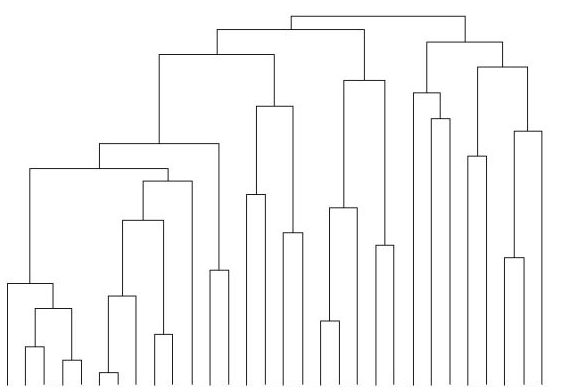
\includegraphics[width=0.8\textwidth]{clustering/dendrogram.png}
\caption{Dendrogramma}
\label{Dendrogram}
}
\end{figure}
Esistono due tipi di clustering gerarchico:
\begin{itemize}
\item clustering divisivo: approccio di tipo top-down che parte dall’analisi dell’intero dataset, rappresentato come il nodo radice del dendrogramma e si occupa di scomporlo ricorsivamente in nodi figli, fino ad arrivare al massimo ad aggiungere nodi impossibili da partizionare ulteriormente, cioè nodi foglia costituiti ognuno da un solo oggetto.
\item clustering agglomeratito: approccio di tipo bottom-up che parte dall’analisi delle foglie dell’albero, cioè le singole istanze, e costruisce un nuovo nodo, cioè il padre, degli oggetti fra loro simili entro una certa soglia. Il processo si conclude quando due o più nodi della struttura si agglomereranno in un unico nodo, che è definito \textit{radice}, corrispondente all’intero insieme dei dati di partenza.
\end{itemize}

Il clustering gerarchico, a differenza del clustering partizionale in cui è utilizzata solo una funzione di dissimilarità tra le istanze per la costruzione di esso, necessita di una funzione di distanza al fine di calcolare quanto "distano" tra loro due insieme di oggetti, sottoinsiemi dell'insieme iniziale di dati. Questo calcolo è necessario ogni volta che si vogliono confrontare due nodi dello stesso dendogramma allo stesso livello di profondità diverso dall’ultimo. Sono di seguito elencati (e descritti concettualmente) i principali metodi per calcolare la distanza tra due insiemi:
\begin{itemize}
\item Metodo single-link: la distanza fra due cluster è uguale alla distanza fra i due oggetti più vicini dei due cluster (un data point per cluster). Matematicamente, questo metodo, considerando la distanza tra i cluster \textit{X} e \textit{Y}, è descritto tramite l'espressione:
\begin{center}
$D(X,Y)$=$\min_{x\in X, y\in Y}$ $d(x,y)$
\end{center}
\item Metodo complete-link: la distanza fra due cluster è uguale alla distanza fra i due oggetti più lontani dei due cluster. Sempre considerando la distanza tra i cluster \textit{X} e \textit{Y}, la descrizione matematica di tale metodo è:
\begin{center}
$D(X,Y)$=$\max_{x\in X, y\in Y}$ $d(x,y)$
\end{center}
\item Metodo average-link: la distanza fra due cluster è data dalla media delle distanze calcolate fra tutte le coppie di oggetti appartenenti a cluster diversi. La formula per il calcolo matematico di tale metodo è la seguente:
\begin{center}
$D(X,Y)$ = $\frac{1}{|X| |Y|}$ $\sum_{x \in X }$ $\sum_{ y \in Y}$ $d(x,y)$
\end{center}
\item Metodo dei centroidi: la distanza fra due cluster è uguale alla distanza fra i centroidi dei due cluster (\textit{X} e \textit{Y}). L'espressione matematica che descrive tale metodo è:
\begin{center}
$$D(X,Y) = d(\hat{c_x}, \hat{c_y})$$
\end{center}
\end{itemize}
\subsection{Clustering concettuale e interpolativo}
Le tecniche tradizionali di clustering permettono di raggruppare istanze di dati che sono tra loro simili. Nel clustering concettuale o \textit{conceptulal clustering} \cite {19a} invece si fornisce in più una interpretazione dei dati che sono stati raggruppati nello stesso insieme. Viene infatti associato a ciascun cluster la sua descrizione concettuale. In questa nuova tecnica di clustering, una nuova istanza viene confrontata con tutte le descrizioni associate ai cluster per stabilire il suo cluster di appartenenza.

Il clustering interpolativo (o \textit{interpolative clustering}) è una forma di apprendimento supervisionato, differentemente del clustering concettuale. Oltre alla descrizione del clustering, viene associato anche un modello predittivo che sta a rappresentare un "riassunto" (\textit{summarization}) dei dati contenuti nel cluster.
\newpage
\section{VARForecaster 1.0/2.0}
In \cite{donato} sono descritte due versioni dell'algoritmo che, avuto in input un insieme di sensori (definito in seguito \textit{dataset}), tramite applicazione del modello VAR effettuano predizione di quelli che potrebbero essere i valori assunti da tali sensori nel futuro. 


\subsection{VARForecaster 1.0}
I sensori effettuano rilevazioni periodicamente e questo porta ad avere un flusso di dati multi-variato, rappresentato, per ogni istante di tempo, attraverso uno snapshot e l'insieme degli snapshot compone il dataset. 

La versione VARForecaster 1.0 è caratterizzata dall'apprendimento di un modello VAR per ogni sensore appartenente alla rete, utilizzando come dati di training la serie storia multi-variata, la quale contiene le rilevazioni effettuate dal sensore.

Questo processo (\cite{donato}) avviene finché c'è uno snapshot da processare e nel dettaglio si compone di:
\begin{enumerate}
\item leggere lo snapshot e memorizzarne i dati;
\item aggiornare la serie storica multi-variata associata ad ogni sensore;
\item apprendere un modello VAR per sensore;
\item effettuare, se possibile, il forecast per ogni sensore.
\end{enumerate}
Durante la terza fase, per ognuno dei sensori, in base ai rispettivi dati di training, viene associato un modello VAR ad ogni sensore, e ciò è possibile se e soltanto se siano stati esaminato un numero di istanti temporali sufficienti alla costruzione dello stesso. Il numero minimo di istanti per la costruzione di tale modello è parametrizzato e l'utente può deciderlo arbitrariamente. Una volta raggiunta la soglia sarà sempre possibile apprendere il modello VAR.

Se il modello VAR è stato appreso è possibile effettuare la previsione (forecast).

Questa si effettua applicando, per ogni sensore, al modello VAR la serie storica dello stesso. È possibile prevedere quanti istanti temporali si vuole, con la premessa che previsioni più "lontane" sono meno precise di quelle immediatamente successive all'istante temporale \textit{t} in oggetto. Per le successive previsioni le equazioni vanno calcolate considerando come ultimo istante di tempo della serie storica la previsione precedentemente effettuata. La quantità di previsioni da effettuare sono a discrezione dell'utente \cite{donato}.

Le fasi di lettura del nuovo snapshot e di aggiornamento delle serie storiche devono tenere conto della probabile presenza di sensori inattivi. 

Per sensore inattivo \cite{donato} si intende un sensore appartenente alla rete che non ha effettuato alcuna rilevazione in quell'istante di tempo per un qualsiasi motivo (disattivazione manuale del sensore, guasto hardware, guasto software$\dots$) e per il quale deve comunque essere mantenuta la finestra di rilevazioni effettuate nel tempo. 

Durante le fasi di esecuzione del sistema tale probabilità viene gestita in maniera diversa \cite{donato}. Infatti, durante la seconda fase, ovvero quella di aggiornamento delle serie temporali viene controllato se per il sensore, precedentemente, sia stata effettuata o meno previsione. Nel caso in cui l'esito sia positivo, si sostituisce la previsione effettuata con ahead = 1 alla rilevazione (non avuta), in caso contrario si "contrassegna" tale sensore con il valore massimo che Java permette per la rappresentazione dei valori Double (definito in seguito \textit{"MAX-VALUE"}). 

In base a questa strategia è naturale che se per un sensore è effettuata una volta previsione sarà sempre possibile effettuarne altre. 

Durante la seconda fase il sistema deve invece verificare che la sua serie storica non contenga il valore significativo di non rilevazione \textit{"MAX-VALUE"}. Nel caso in cui tale valore sia presente, non è possibile effettuare apprendimento del modello VAR. 

Durante la quarta ed ultima fase, il sistema deve solo controllare che per il sensore in oggetto sia stato appreso il modello VAR, in caso positivo effettuerà la previsione, altrimenti no.
\subsection{VARForecaster 2.0}
VARForecaster 2.0 (\cite{donato}) adatta il \textit{clustering interpolativo} al fine di raggruppare sensori per i quali si mantiene un sommario relativamente alla finestra temporale da usare per la costruzione del modello VAR. Questa struttura, oltre ad includere le condizioni di split scelte in base alle autocorrelazioni spaziali che intercorrono tra i sensori, è dinamica nel tempo. 

Per ciascun cluster è poi appreso un modello VAR in base alla serie storica multi-variata che lo rappresenta, determinata dalla media assunta da ciascuna variabile all'interno del cluster di appartenenza, e con la combinazione lineare tra quest'ultima ed il modello stesso è in seguito effettuata una predizione dei valori futuri per ciascuna delle istanze che ricadono all'interno di quel cluster \cite{donato}.

L'autocorrelazione spaziale altro non è che un cluster territoriale di valori simili. Se a valori simili nelle istanze corrisponde una vicinanza spaziale si è in presenza di autocorrelazione spaziale positiva, al contrario l'autocorrelazione viene definita come negativa. Tali valori sono fondamentali per la scelta del partizionamento ottimale dei sensori.

I punti cardine di questa versione sono:
\begin{enumerate}
\item fase di apprendimento della struttura Clustering Tree (CT in seguito);
\item fase di modifica incrementale del CT;
\item fase di apprendimento del modello VAR;
\item fase di forecast.
\end{enumerate}

\subsubsection{Fasi di apprendimento e modifica incrementale del CT}
Un Clustering Tree (\cite{donato}) è una struttura ad albero utilizzata per rappresentare uno snapshot  mediante un insieme di cluster organizzati gerarchicamente su di esso.

In questo modo per ogni sensore ricadente all'interno del nodo in oggetto esiste una sequenza di cluster $C_{i0}$, $C_{i1}$, $\dots$, $C_{ir}$ nei quali la partizione all'interno del quale si trova tale sensore è inclusa. Per permettere ciò, è necessaria che sia rispettata la condizione di inclusione $C_{i0}$ $\supseteq$ $C_{i1}$ $\supseteq$ $\dots$ $\supseteq$ $C_{ir}$. 
\

Ogni cluster $C_{i0}$, $C_{i1}$, $\dots$, $C_{ir}$ è associato ad un nodo $n_{i0}$, $n_{i1}$, $\dots$, $n_{ir}$ e ogni nodo $n_{ij}$ appartenente al CT è un figlio diretto del nodo $n_{ij-1}$ (j = 1, $dots$, r). Il nodo radice è definito da $n_{i0}$, dove 0 indica appunto il livello del nodo all'interno dell'albero.

Apprendere un CT quindi vuol dire effettuare un processo di clustering sullo snapshot ricevuto in ingresso e associare una struttura ad albero ad esso, in modo tale che ogni nodo corrisponda ad un cluster. 

Nel dettaglio l'algoritmo per l'apprendimento del CT lavora in maniera ricorsiva secondo un approccio top-down, ricevendo in input uno snapshot, partizionandolo (in base ai valori assunti dai sensori e alle autocorrelazioni spaziali che intercorrono tra di essi) e fermandosi quando sono soddisfatti dei criteri di stop. 

Essendo questo un algoritmo ricorsivo con criterio top-down, su ogni nuovo cluster(/nodo) \textit{c} trovato, si tenta di apprendere altri sotto-alberi con radice \textit{c}. Tale processo si ferma se ci sono troppe poche istanze in \textit{c} oppure se c'è troppo adattamento ai dati e quindi si rischia il problema dell'over-fitting dell'albero.

Il processo principale di questo algoritmo è la scelta delle condizioni di split. Essendo lo scopo fondamentale del clustering la massimizzazione della riduzione della varianza degli indicatori locali dell'autocorrelazione spaziale all'interno dei cluster, le condizioni di split indicano i migliori accoppiamenti attributo-valore in grado di diminuire tale valore. La migliore tra tutte le condizioni è quella scelta e sarà utilizzata come decisione per dividere (partizionare) lo snapshot (o la partizione di esso se ci troviamo in un nodo che non sia la radice dell'albero).

Al termine di questa fase ad ogni nodo sarà stata associata una serie storica multi-variata, rappresentante i valori assunti nel tempo da tutti gli attributi, per ciascuna istanza che ricade nel cluster, contenente un solo valore per attributo. Tale valore è la media di tutti i valori assunti da quell'attributo da tutti i sensori presenti nel cluster.

La fase incrementale nell'apprendimento del CT lo adatta al nuovo snapshot ricevuto in input. Per fare ciò si avvale di un algoritmo ricorsivo con metodo top-down il quale attraversa l'albero e si preoccupa di trovare quei cluster che presentano un sostanziale cambiamento nella proprietà di autocorrelazione spaziale. 

Questo processo di divide nella fase di pruning e nella fase di apprendimento di nuovi sotto-alberi.

La fase di pruning interessa solo i nodi di decisione e li pota se non riconosce un'effettiva convenienza nel mantenimento di tale split. Potare un nodo \textit{n} significa cancellare i sotto-alberi che aveno \textit{n} come radice e trasformare quindi \textit{n} stesso in foglia. Tale procedimento non intacca la serie storica multi-variata associata al nodo ne tanto meno le istanze che ricadono al suo interno e quindi i valori medi, minimi e massimi assunti dalle feature nel cluster rimangono invariate. 

La fase di apprendimento di nuovi sotto-alberi, successiva a quella di pruning, interessa invece soltanto i nodi foglia. Partendo da essi infatti, l'algoritmo ricorsivo cerca di capire se sia possibile e conveniente apprendere dei nuovi cluster.
Nel caso in cui siano appresi nuovi cluster a partire dal nodo \textit{n}, la radice del nuovo sotto-albero sarà \textit{n} e le serie storiche multi-variate associate a questi nodi saranno, fino all'istante \textit{t-1} copiate dalla serie temporale multi-variata di \textit{n}, mentre per l'istante temporale corrente, ovvero \textit{t}, il valore sarà calcolato in base alle istanze che realmente ricadono all'interno del cluster.  
\subsubsection{Fasi di apprendimento del modello VAR e predizione}
Nel momento in cui l'apprendimento incrementale di CT è terminato (per quello snapshot), per ogni cluster foglia, si prova ad apprendere un modello VAR. Questo viene appreso sulla base dei valori presenti all'interno della serie storica multi-variata ad esso associata e per poter avviare questo meccanismo vengono richiesti un minimo numero di istanti temporali all'interno di tale serie. Il numero minimo di medie multi-variate richieste all'interno della serie è arbitrario ed è stato parametrizzato. Questo perché tale decisione dipende dalle necessità dell'utente. Tutto ciò implica che una volta raggiunta la soglia minima di istanti temporali processati è sempre possibile apprendere il modello VAR.

Nella fase di forecast vengono recuperati per ogni nodo il modello VAR ad esso associato e in base allo snapshot attuale, questo viene applicato all'istanza, quindi al sensore, corretto. 

Per ciò che riguarda l'eventuale presenza di sensori inattivi, questa influisce soltanto sulla fase di previsione, in quanto, durante la fase di aggiornamento delle serie temporali ci si comporta come fatto in VARForecaster 1.0, per la fase di apprendimento dell'albero vengono considerati soltanti i sensori attivi e per l'apprendimento del modello VAR viene utilizzata la serie temporale associata al cluster e quindi eventuali valori non rilevati, non facendo parte di tale cluster, non ne influenzerebbero la costruzione. 

L'applicazione, durante la fase di previsione, deve controllare, per ogni sensore, che la propria serie storica multi-variata non contenga valori non significativi (\textit{MAX-VALUE}) negli istanti temporali coinvolti nella previsione. Nel caso in cui tale riscontro sia positivo per quel sensore sarà effettuato forecast, in alternativa no. In base a tale assunzione, se per un sensore viene effettuato forecast una volta, sarà sempre possibile effettuarne altri.
\chapter{VARForecaster 2.1/2.2}
In questo capitolo sono descritte le versioni dell'algoritmo (descritto nel par. 2.4) progettate ed implementate in questo lavoro di tesi. 

Si ricorda che (come descritto nel par. 1.1) l'algoritmo è stato esteso al fine di calcolare gli aggregati dei dati in tempo reale (media o mediana) piuttosto che ricorrere ad approssimazione degli stessi e utilizzare un meccanismo di smoothing esponenziale per determinare il modello di clustering sulla base dei valori geofisici attesi nella rete all'istante {\bfseries t+1} piuttosto che sulla base dei valori osservati all'istante {\bfseries t}. La motivazione è l'identificazione di una soluzione che realizza il miglior bilanciamento tra accuratezza e efficienza.
\section{VARForecaster 2.1}
L'albero è costruito in maniera incrementale (par. 2.4), ovvero, ad ogni nuovo snapshot di dati all'interno dello stream, l'algoritmo controlla che le condizioni di split in base alle quali è stato costruito il modello di clustering all'istante t-1 siano compatibili con i dati raccolti all'istante t.

A tale scopo, per ogni nuovo snapshot, l'albero è aggiornato eseguendo una fase di pruning e poi di ri-apprendimento dell'albero sulla base dei nuovi valori ricevuti. 

Il pruning è un processo ricorsivo nel quale vengono analizzati i nodi di split, i quali sono potati se la loro condizione di split non porta ad una reale riduzione della varianza degli indicatori locali di autocorrelazione spaziale sui nuovi record. 

Nel caso in cui venga applicata la potatura, il nodo di split viene sostituito con un nodo foglia, al cui interno ricadranno tutte le istanze precedentemente appartenenti al nodo di split. 

La fase di ri-apprendimento dell'albero, al contrario di quella di pruning, prende in considerazione i nodi foglia, è infatti in questa fase che l'algoritmo VARForecaster tenta di apprendere nuovi sotto-alberi.

Secondo la versione 2.0 dell'algoritmo, nel momento in cui viene appreso un nuovo nodo, a questo viene assegnata, nella struttura dati che tiene traccia delle medie multi-variate assunte da ogni cluster (cioè la struttura dati \textit{Feature Window}), la media precedente calcolata per il suo nodo padre (vedi par. 2.4). 

\subsubsection{Aggregazione in tempo reale}
Al fine di migliorare la rappresentatività dei dati usati per l'apprendimento del modello VAR, si è pensato di ricostruire, per ogni nuovo nodo appreso, la media multi-variata ad esso associata, in modo tale da mantenere un'aggregato multi-variato calcolato sulla base dei reali valori assunti dalle istanze dei sensori che ricadono all'interno del cluster foglia.

Questo processo è realizzato all'interno della struttura dati \textit{Node} e si sviluppa nei seguenti passi:
\begin{itemize}
\item Per ogni sensore appartenente al cluster foglia:
\begin{itemize}
\item viene letta la serie storica multi-variata ad esso associato;
\item per ogni caratteristica (\textit{Feature}) presente all'interno della serie:
\begin{itemize}
\item per ogni istante temporale precedente a t, viene letto il valore corrispondente e lo si somma agli altri valori letti per la caratteristica in esame;
\item viene incrementato un contatore, il quale sarà necessario per definire quanti istanti temporali sono stati sommati.
\end{itemize}
\end{itemize}
\end{itemize}

Alla fine di tale procedimento, per ogni sensore, sono calcolati, in maniera separata, la somma ottenuta per ogni \textit{Feature} ed il valore del contatore a quella caratteristica associata.

Questi valori rappresentano la media, per ogni \textit{Feature}, delle rilevazioni effettuate fino all'istante t dall'insieme di sensori che ricadono all'interno del cluster foglia.
Tali valori sono poi accodati all'insieme delle rilevazioni precedentemente effettuate dal sensore, per ogni singola \textit{Feature}, nella struttura dati \textit{Feature Window}. 

\subsubsection{Problematiche}
Nel momento in cui si prova a definire un'aggregato multi-variato per un cluster si può incorrere in due inconvenienti:
\begin{itemize}
\item Sensori inattivi;
\item Presenza di outliers;
\end{itemize}
Sono di seguito descritte le modalità secondo le quali è stato possibile risolvere entrambi i problemi.
\subsubsection{Sensori inattivi}
Nel calcolo della media, come specificato in precedenza, vengono considerate tutte le rilevazioni presenti all'interno della finestra temporale associata al sensore. 

Se tale sensore in passato, anche per un singolo istante temporale \textit{$t_{x}$}, non ha effettuato alcuna rilevazione, nella struttura dati \textit{Feature Window} ad esso associata, per l'istante \textit{$t_{x}$}, è salvato il valore massimo che Java permette per rappresentare una variabile di tipo Double (di seguito definito come \textit{"MAX-VALUE"}).


Se si prendesse in considerazione tale valore nel calcolo della media, quest'ultima risulterebbe definitivamente influenzata. Per evitare ciò, nel momento in cui si calcola la media, si controlla che il valore rilevato non sia \textit{"MAX-VALUE"}.
Nel caso in cui si incorre in tale valore, il sensore incriminato, non viene considerato per il calcolo della media e il contatore non subisce alcuna modifica.
 
\subsubsection{Presenza di outliers}
Data la varietà di dati misurati e la distribuzione geografica dei sensori, è possibile che tra le rilevazioni effettuate possano esserci uno o più ouliers. 

Un outlier è un valore anomalo e aberrante; un valore quindi chiaramente distante dalle altre osservazioni disponibili \cite{14a} 

Data la struttura di questi dati, che sarebbero assolutamente fuorvianti in caso di aggregati costruiti tramite l'utilizzo della media, è stato messa a disposizione dell'utente, come parametro per il lancio del software, la possibilità di scegliere se calcolare il suddetto aggregato con l'utilizzo della mediana.

In statistica, in particolare in statistica descrittiva, data una distribuzione di un carattere quantitativo oppure qualitativo ordinabile (ovvero le cui modalità possano essere ordinate in base a qualche criterio), si definisce la \textbf{mediana} (o \textbf{valore mediano}) come il valore assunto dalle unità statistiche che si trovano nel mezzo della distribuzione. 

Se si procede al riordinamento delle unità in base ai valori crescenti del carattere da esso detenuto, in sostanza la mediana bipartisce la distribuzione in due sotto-distribuzioni: la prima a sinistra della mediana (costituita dalla metà delle unità la cui modalità è minore o uguale alla mediana) e la seconda a destra della mediana costituita dalla metà delle unità la cui modalità è maggiore o uguale alla mediana). Tecnicamente si afferma che la mediana è il valore per il quale la frequenza relativa cumulata vale (o supera) 0,5. 

Per calcolare la mediana di \textit{n} dati \cite{15a} 
\begin{itemize}
\item si ordinano gli \textit{n} dati in ordine crescente;
\item se il numero di dati è dispari la mediana corrisponde al valore centrale, ovvero al valore che occupa la posizione \textbf{$\frac{n+1}{2}$};
\item se il numero \textit{n} di dati è pari, la mediana è stimata utilizzando i due valori che occupano la posizione \textit{$\frac{n}{2}$} e \textit{($\frac{n}{2}$ + $1$)}
\end{itemize}

A livello implementativo, la differenza fondamentale tra il calcolo degli aggregati multi-variati tramite media rispetto a farlo con la varianza, risiede nell'utilizzo di una struttura dati in cui vengono memorizzati i valori di ogni serie uni-variata per istante temporale \textit{t}.

Da questa struttura si va poi a leggere il valore centrale, ovvero quello corrispondente alla mediana, per poi continuare ad operare come nel caso della media. Nel caso in cui invece il numero \textit{n} di dati sia dispari, si provvede alla lettura dei due valori centrali e all'utilizzo della media per il calcolo del valore mediano.

\subsubsection{Caso limite}
Esiste, in maniera remota, la possibilità che tutti i sensori che ricadono in un cluster foglia, non abbiano mai effettuato alcuna rilevazione, fino all'istante temporale \textit{t} in esame. 

Per la gestione di questa casistica limite si è preferito quindi accodare un valore \textit{"MAX-VALUE"}, come quello presente in caso di sensore inattivo.

Così facendo è in seguito catturata e gestita un'eccezione che non permette il forecast.


\subsubsection{Conseguenze}
A causa della rielaborazione degli aggregati multi-variati in caso di apprendimento di un nuovo nodo, le serie storiche di ciascun cluster foglia risultano essere ora reali, ovvero adattate alle istanze che realmente ricadono all'interno di tale cluster. Come conseguenza primaria si ha quindi, che la costruzione del modello VAR rispecchierà in maniera maggiore la situazione reale del cluster.

La possibilità di scegliere se costruire gli aggregati con la media oppure con la varianza verrà data all'utente utilizzatore del software grazie ad una parametrizzazione della stessa.
\medskip
\medskip
\medskip
\medskip

Nella prossima sezione si riportano i diagrammi di classe e di sequenza relativi alla progettazione di VARForecaster 2.1.
\newpage
\subsection{Progettazione}
In questa sezione sono illustrate, tramite diagrammi UML (Unified Modeling Language) le variazioni progettate in questo lavoro di tesi dell'algoritmo VARForeacaster 2.1. Precisamente sono presenti: diagramma dei package, diagrammi delle classi e diagrammi di sequenza. Ognuno di essi è seguito da una descrizione.
\subsubsection{Diagramma dei package}
\begin{figure}[H]
\textbf{
\centering
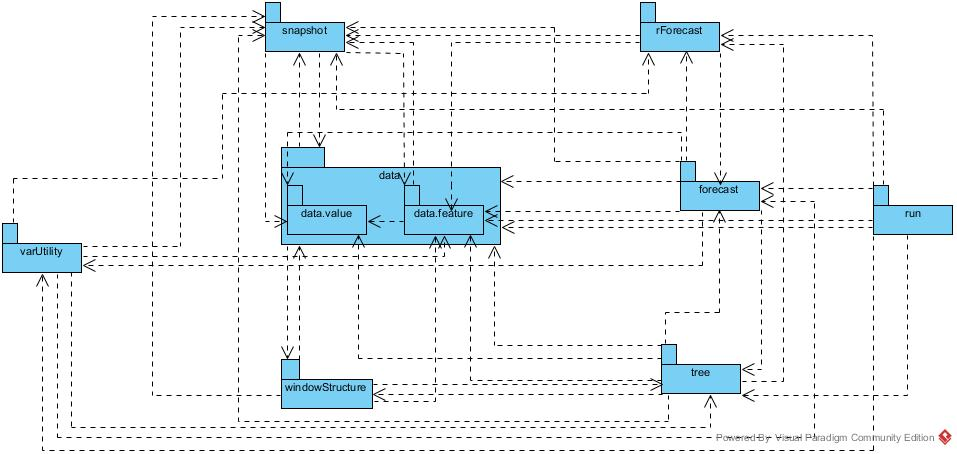
\includegraphics[width=0.8\textwidth]{RealAggregate/Package_Diagram.jpg}
\caption{RealAggregate Package Diagram}
\label{RAPD}
}
\end{figure}
Nella Fig.~\ref{RAPD} sono descritti le principali relazioni che intercorrono tra i package presenti all'interno del software, ovvero come un package è in relazione con un altro. 

A tali relazioni non è stata apportata alcuna modifica.
\newpage
\subsubsection{Diagrammi delle classi}
\begin{figure}[H]
\textbf{
\centering
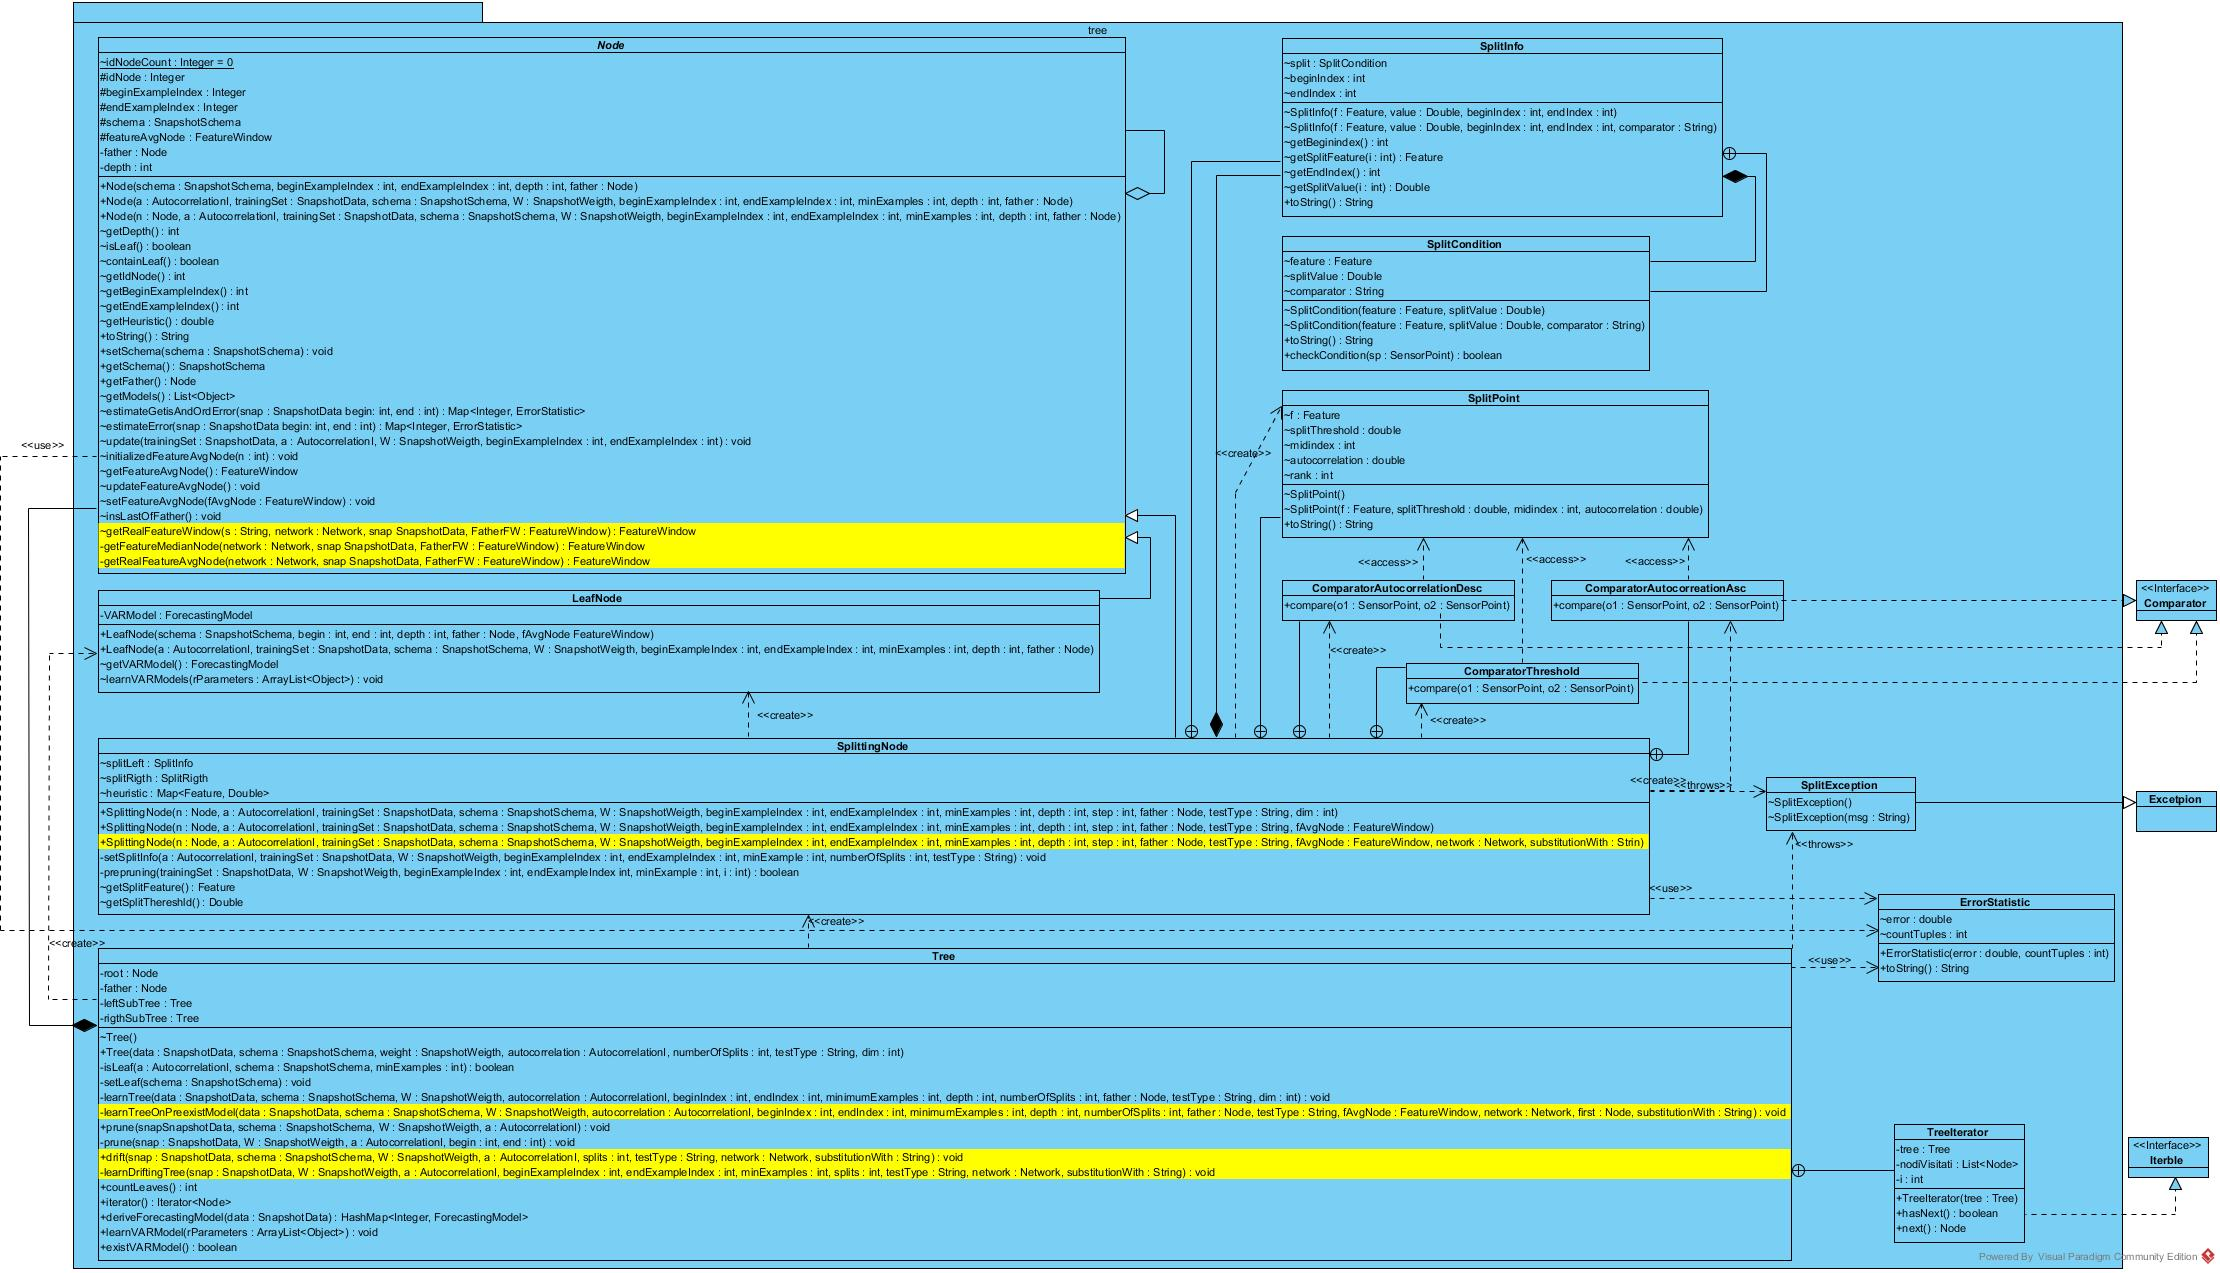
\includegraphics[width=\paperwidth,height=\paperheight/2, angle = 90]{RealAggregate/Tree_Class_Diagram.jpg}
\caption{RealAggregate Tree Class Diagram}
\label{RACD}
}
\end{figure}
Come è possibile notare, in Fig.~\ref{RACD}, ci sono dei metodi in giallo. Questi sono i metodi aggiunti rispetto alla versione VARForecaster 2.0. 

Tali metodi hanno la responsabilità di calcolare gli aggregati reali e sono utilizzati vicendevolmente rispetto al parametro ricevuto in input dall'utente. Precisamente:
\begin{itemize}
\item getRealFeatureWindow: è il metodo che ha la responsabilità di leggere il parametro che determina il tipo di funzione da applicare per calcolare l'aggregato (media o mediana), di chiamare il metodo corretto e restituire la struttura contenente i dati aggregati aggiornati;
\item getFeatureMedianNode: è il metodo che ha il compito di calcolare l'aggregato reale con la funzione \textit{"mediana"};
\item getRealFeatureAvgNode: è il metodo che ha la responsabilità di calcolare l'aggregare reale con la funzione \textit{"media"}.
\end{itemize}

Tali metodi sono utilizzati, come detto nel par. 3.1, nella fase di apprendimento incrementale del clustering, quindi per l'esattezza nel metodo privato \textit{learnTreeOnPrexistModel} nella classe \textit{Tree}.

Queste modifiche sono esplicitate chiaramente, nella seguente sotto-sezione, dai diagrammi di sequenza. 
\newpage
\begin{figure}[H]
\textbf{
\centering
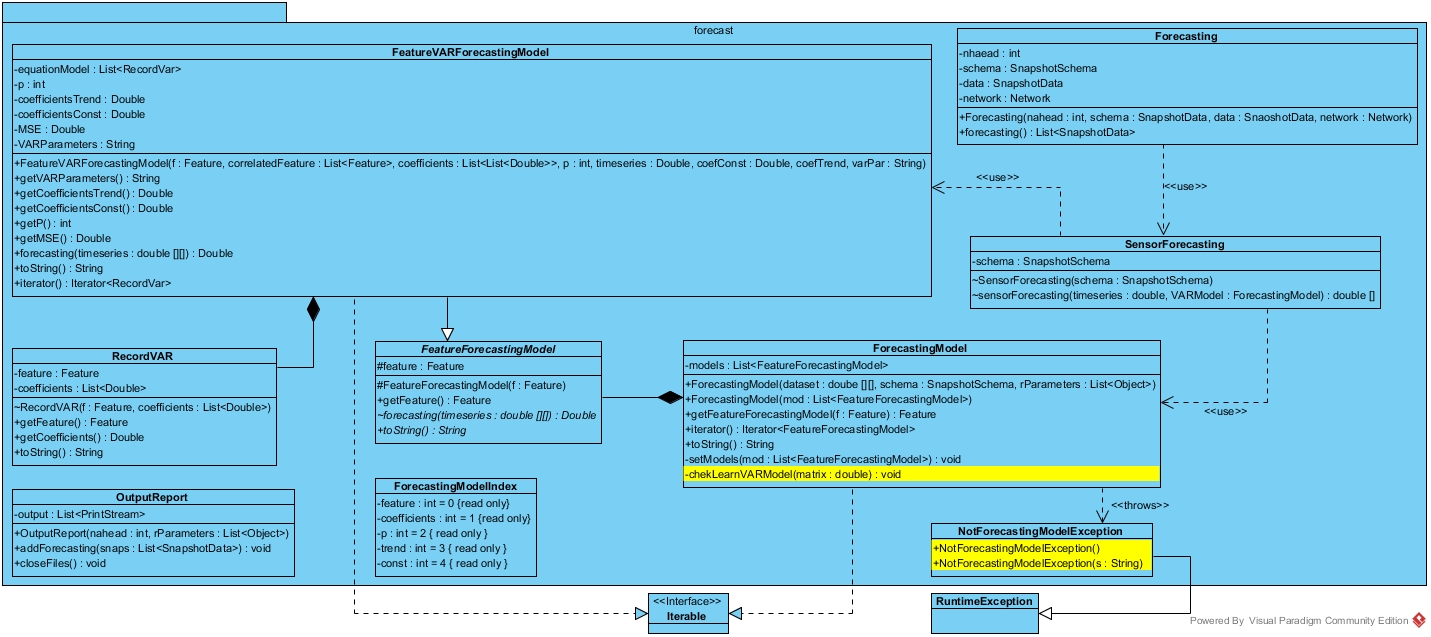
\includegraphics[width=\paperwidth,height=\paperheight/2, angle = 90]{RealAggregate/Forecast_Class_Diagram.jpg}
\caption{RealAggregate Forecast Class Diagram}
\label{FCD}
}
\end{figure}

In Fig.~\ref{FCD} sono mostrate le modifiche al package \textit{Forecast}. Esse sono state apportate in quanto è necessario controllare se nel modello VAR associato ad ogni nodo sono presenti \textit{"MAX-VALUE"} i quali indicherebbero l'impossibilità di effettuare previsione.

Per gestire questa eventualità è stata aggiunta l'eccezione \textit{NotForecastingModelException} la quale è catturata, nel caso in cui sia trovato il valore incriminato, dal metodo \textit{checkLearnVARModel}.
\newpage




\subsubsection{Diagrammi di sequenza}
\begin{figure}[H]
\textbf{
\centering
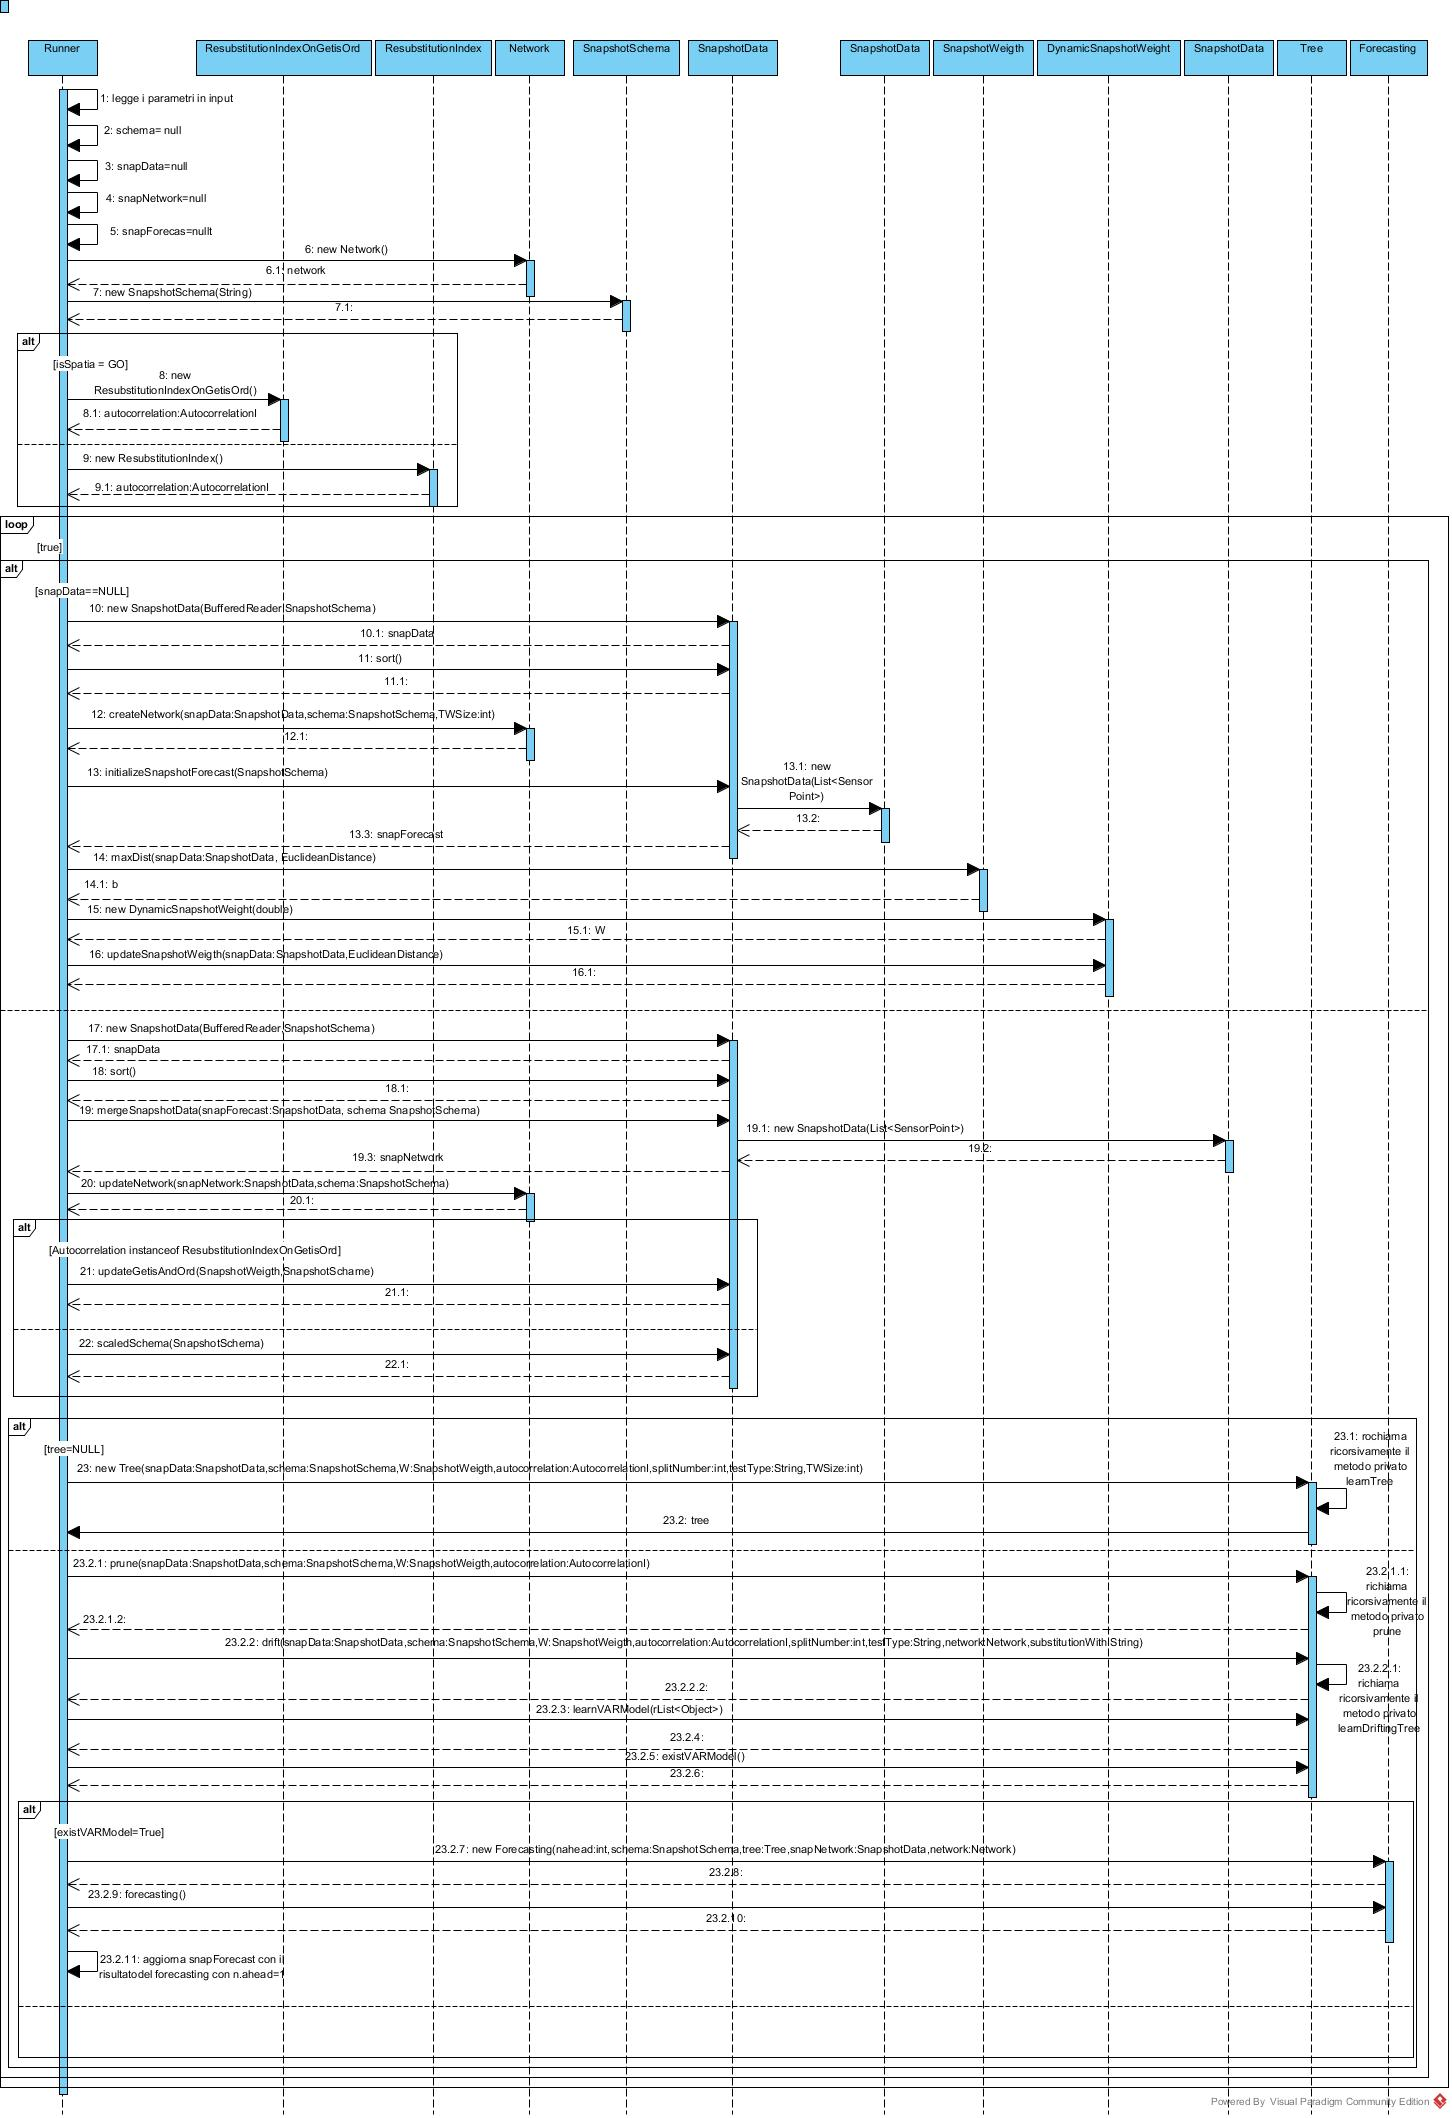
\includegraphics[width=0.8\textwidth]{RealAggregate/run.jpg}
\caption{Run VARForecaster 2.1}
\label{run}
}
\end{figure}
\newpage
\begin{figure}[H]
\textbf{
\centering
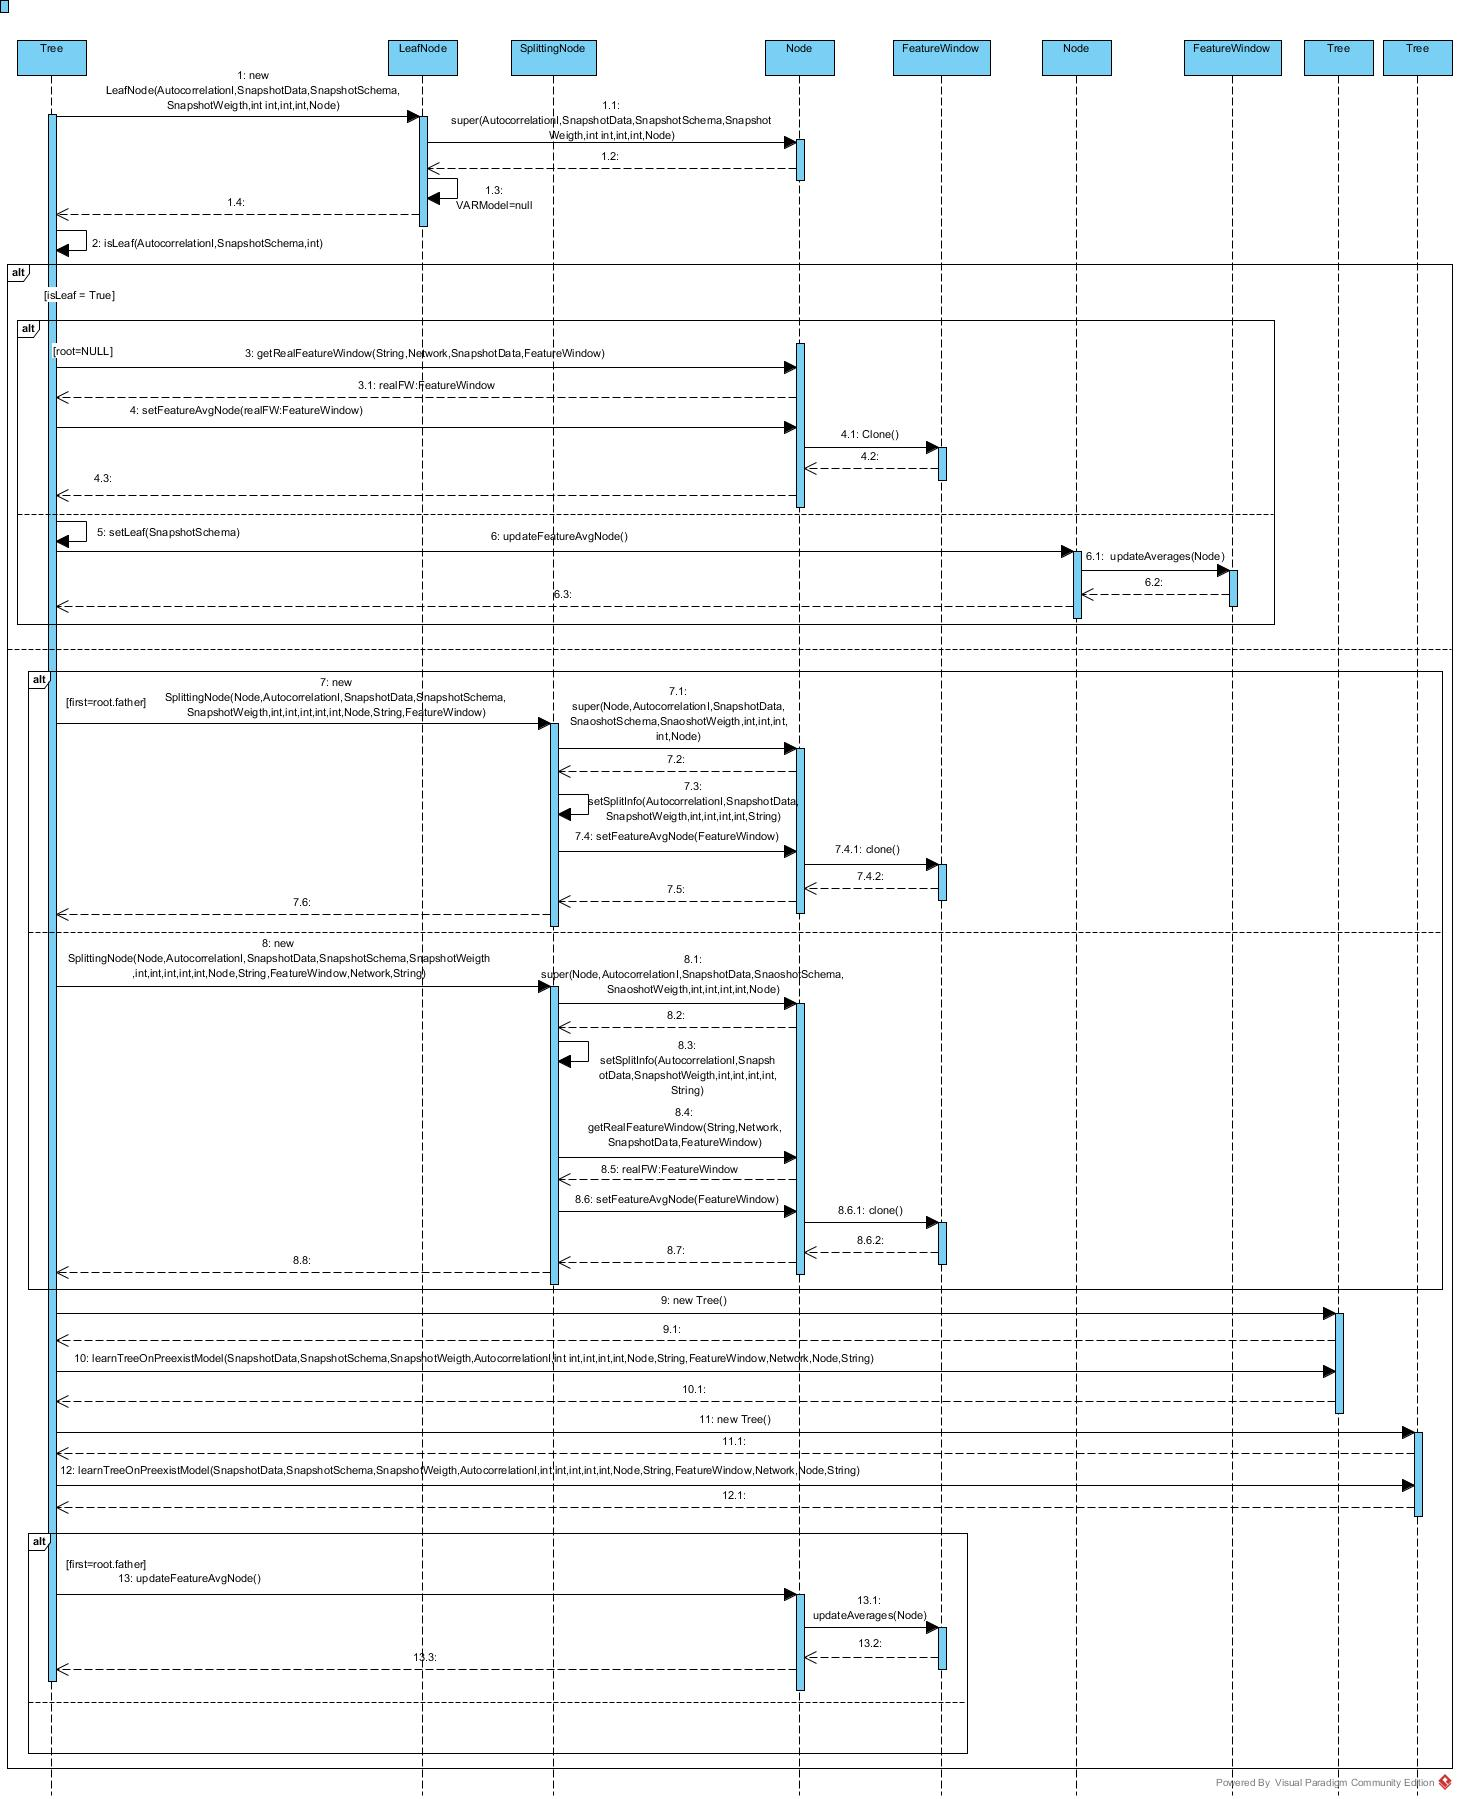
\includegraphics[width=0.8\textwidth]{RealAggregate/learnTreeOnPrexistModel.jpg}
\caption{Riapprendimento \textit{CT} VARForecaster 2.1}
\label{LTOPM}
}
\end{figure}
\newpage
\begin{figure}[H]
\textbf{
\centering
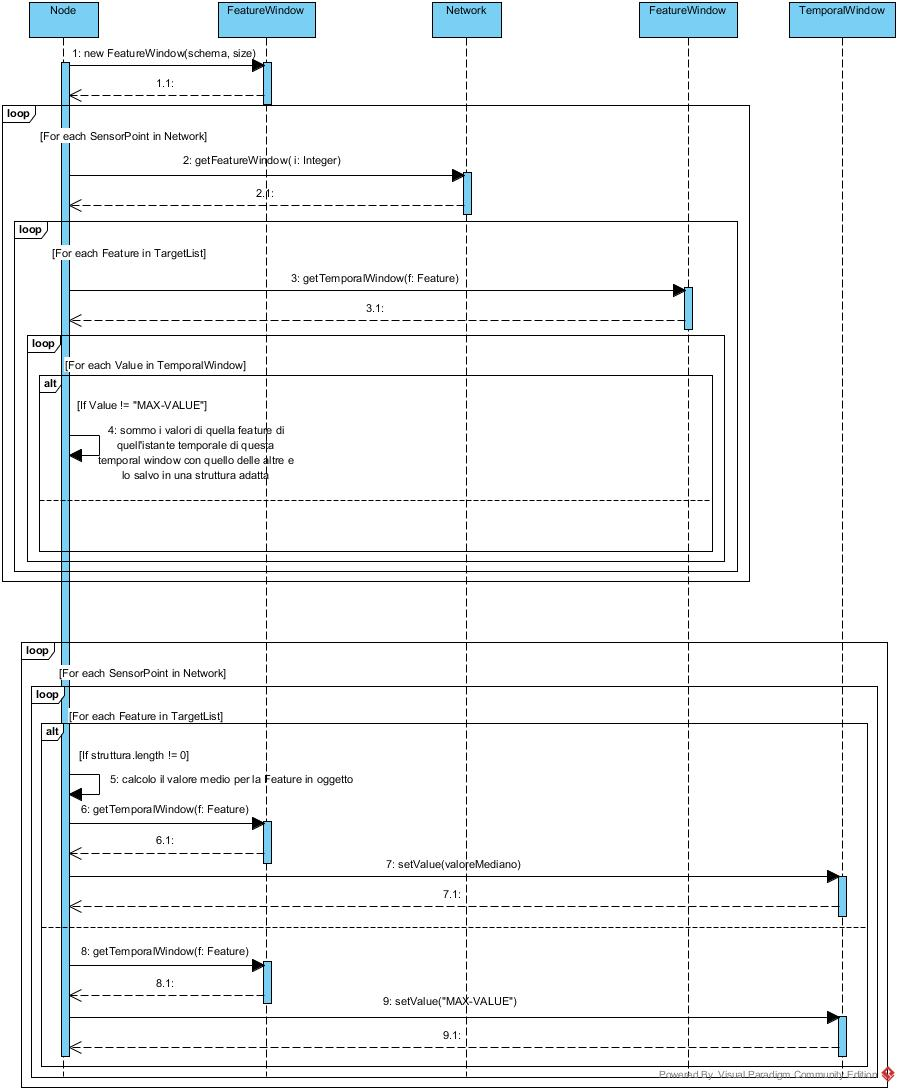
\includegraphics[width=0.8\textwidth]{RealAggregate/Avg.jpg}
\caption{Apprendimento aggregato con media}
\label{AVG}
}
\end{figure}
\newpage
\begin{figure}[H]
\textbf{
\centering
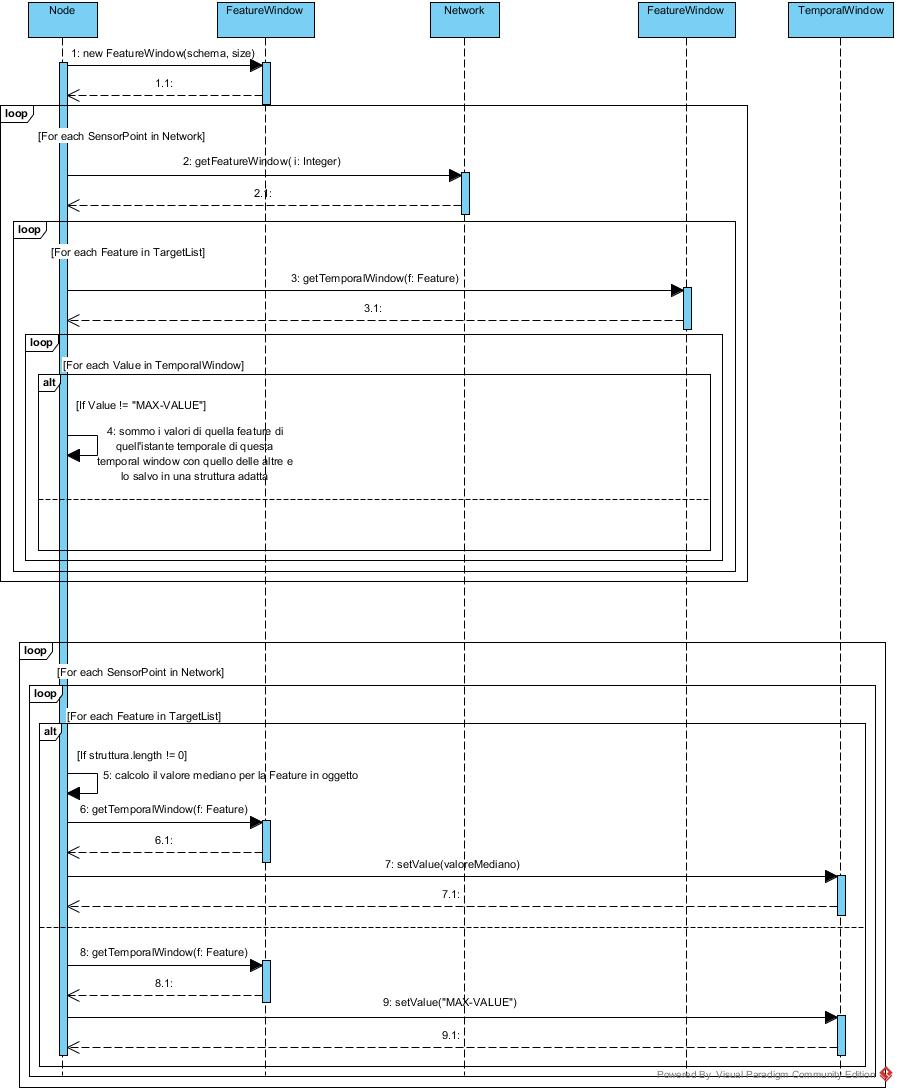
\includegraphics[width=0.8\textwidth]{RealAggregate/Median.jpg}
\caption{Apprendimento aggregato con mediana}
\label{Median}
}
\end{figure}
\newpage
\begin{figure}[H]
\textbf{
\centering
\includegraphics[width=0.8\textwidth]{RealAggregate/Var.jpg}
\caption{Apprendimento modello VAR VARForecaster 2.1}
\label{VAR}
}
\end{figure}
\newpage
\section{VARForecaster 2.2}
VARForecaster 2.0 basa il partizionamento dei sensori sullo snapshot predetto usando un meccanismo di smoothing esponenziale.

L'albero, nelle versioni 2.0 e 2.1, viene appreso su ogni snapshot ricevuto in input all'istante temporale \textit{t} mentre in questa versione è appreso sulla previsione effettuata sui dati avuti nell'istante \textit{t-1} tramite l'utilizzo della tecnica di smoothing esponenziale. 

Per effettuare tale operazioni si sono rese necessarie alcune modifiche alla struttura del sistema che possono essere riassunte in 2 fasi:
\begin{enumerate}
\item creazione dello snapshot previsto attraverso lo smoothing esponenziale (in seguito def. \textit{snapSmoot});
\item apprendimento incrementale del \textit{CT};
\end{enumerate}
Nei successivi paragrafi sono descritte entrambe le fasi con particolare attenzione alle modifiche effettuate.
\subsubsection{Creazione dello \textit{snapSmoot}}
La fase di creazione dello \textit{snapSmoot} avviene ogni qualvolta si processa un nuovo snapshot. Tale fase si preoccupa di leggere lo snapshot dell'istante temporale \textit{t} in esame, precedentemente ricevuto in input, e processarlo al fine di produrre uno snapshot di previsioni di quelli che potrebbero essere i valori assunti da ciascuna feature di ciascuna istanza presente al suo interno. 

Questo processo si compone di due casistiche:
\begin{itemize}
\item si tratta del primo istante temporale contenente i valori rilevati dai sensori;
\item è un istante temporale successivo al primo, quindi abbiamo già applicato lo smoothing in precedenza.
\end{itemize}

Nel caso in cui sia stia analizzando il primo istante temporale, il sistema si preoccupa di clonare tutti i sensori ricevuti in input nello \textit{snapSmoot}. Questo è dovuto al fatto che il passo base per il calcolo dello smoothing esponenziale è ottenuto con la copia dei dati ricevuti in ingresso. 

Nel caso in cui invece si stia analizzando un istante temporale successivo al primo, il sistema ha la responsabilità di trovare, tra i sensori presenti nello \textit{snapSmoot} di \textit{t-1}, i sensori che nell'istante temporale \textit{t} hanno effettivamente effettuato una rilevazione e combinarli applicando il metodo di \textit{smoothing esponenziale di Brown}.

\subsubsection{Sensori inattivi nella creazione dello \textit{snapSmoot}}
Come nel caso della versione VARForecaster 2.1, i sensori inattivi rappresentano un eventuale problematica da gestire. 

Come precedentemente specificato, il sistema deve trovare tra i sensori presenti nello \textit{snapSmoot} di \textit{t-1} quelli che hanno effettivamente rilevato dei dati nell'istante temporale \textit{t} in considerazione. Ciò implica due conseguenze: 
\begin{enumerate}
\item potrebbero esserci sensori presenti all'interno di \textit{snapSmoot} ma non presenti all'interno dello snapshot attuale;
\item potrebbero esserci sensori presenti nello snapshot attuale ma non presenti nello \textit{snapSmoot}.
\end{enumerate}
Per la gestione di (1) è stato scelto di ignorare tali sensori in quanto il processo di smoothing, prendendo in considerazione gli istanti temporali precedenti a \textit{t} avrebbe un valore mancante, il quale condizionerebbe tutto il meccanismo.

Per la gestione di (2), per lo stesso motivo appena citato, si è preferito far ripartire il processo di smoothing dal "passo base" e quindi di clonare il sensore reale.
\subsubsection{Apprendimento incrementale del \textit{CT}}
In questa fase di progetto si è fatta molta attenzione a distinguere due processi: 
\begin{itemize}
\item aggiornamento dei dati relativi ai cluster
\item costruzione dell'albero
\end{itemize}
Per aggiornamento dei dati relativi ai cluster si intende quella fase in cui vengono aggiornati, per ogni nodo, relativamente al cluster a cui fanno riferimento, i valori delle feature di ogni sensore. Questo vuol dire che i dati presenti in ogni nodo sono riferiti ai valori realmente rilevati dai sensori che ricadono in quel cluster e non ai valori predetti con lo smoothing.

La costruzione dell'albero invece avviene sulla base dei valori predetti con lo smoothing. Ciò indica che l'albero sarà adattato ai valori previsti per quel gruppo di sensori che ricade nel nodo in oggetto. 

Nella fase di crescita incrementale dell'albero questo vuol dire che non soltanto la fase di apprendimento ha subito modifiche ma anche quella di potatura. 

In questa fase si applica l'operatore di pruning sulla base dei valori predetti per lo snapshot \textit{t-1} presenti in \textit{snapSmoot} in quanto l'albero è stato appreso sulla base dei valori presenti in esso. 

Tale processo avviene facendo attenzione, nella fase di aggiornamento dei dati in base ai valori ricevuti dal nuovo snapshot, a mantenere nel nodo i valori associati alle reali rilevazioni ottenute dai sensori che ricadono in quel nodo, mentre per il computo dell'autocorrelazione spaziale e per le decisioni di pruning, vengono utilizzati i valori presenti in \textit{snapSmoot}.

La fase di apprendimento, detta anche \textit{drift}, è la parte maggiormente modificata. Questo avviene perché le decisioni di split devono essere apprese in base allo \textit{snapSmoot}, di conseguenza l'applicazione deve preoccuparsi di lavorare parallelamente su entrambi gli snapshot (\textit{snapSmoot} e lo snapshot contenente i valori realmente rilevati).

\subsubsection{Metodo scelto e parametrizzazione}
Il metodo di smoothing utilizzato in questo progetto di tesi è il \textit{metodo di Brown}. Si riporta la l'espressione matematica di tale metodo:

\medskip
Passo ricorsivo
\begin{center}
$Y_{t}$ = $\alpha$ $x_{t}$ + (${1 - \alpha }$) $Y_{t-1}$
\end{center}
Passo base
\begin{center}
$Y_t$ = $x_t$
\end{center}
dove, in questo progetto di tesi:
\begin{itemize}
\item $x_t$ è lo snapshot contenente i valori realmente rilevati dai sensori;
\item $Y_{t-1}$ è lo \textit{snapSmoot} ottenuto dall'applicazione della funzione di smoothing esponenziale sul precedente snapshot contente i valori reali ($x_{t-1}$);
\item $\alpha$ è il parametro di smoothing.
\end{itemize}
La scelta del parametro di smoothing è arbitraria e affidata all'utente, ma per non adattare troppo i dati previsti a quelli reali o a quelli precedente previsti è consigliabile mantenersi entro 0.4 $\leq$ $\alpha$ $\leq$ 0.6.
\newpage
\subsection{Progettazione}
In questa sezione sono presentati e descritti i diagrammi di classe e di sequenza che descrivono VARForecaster 2.2.
\subsubsection{Diagrammi di classe}
\begin{figure}[H]
\textbf{
\centering
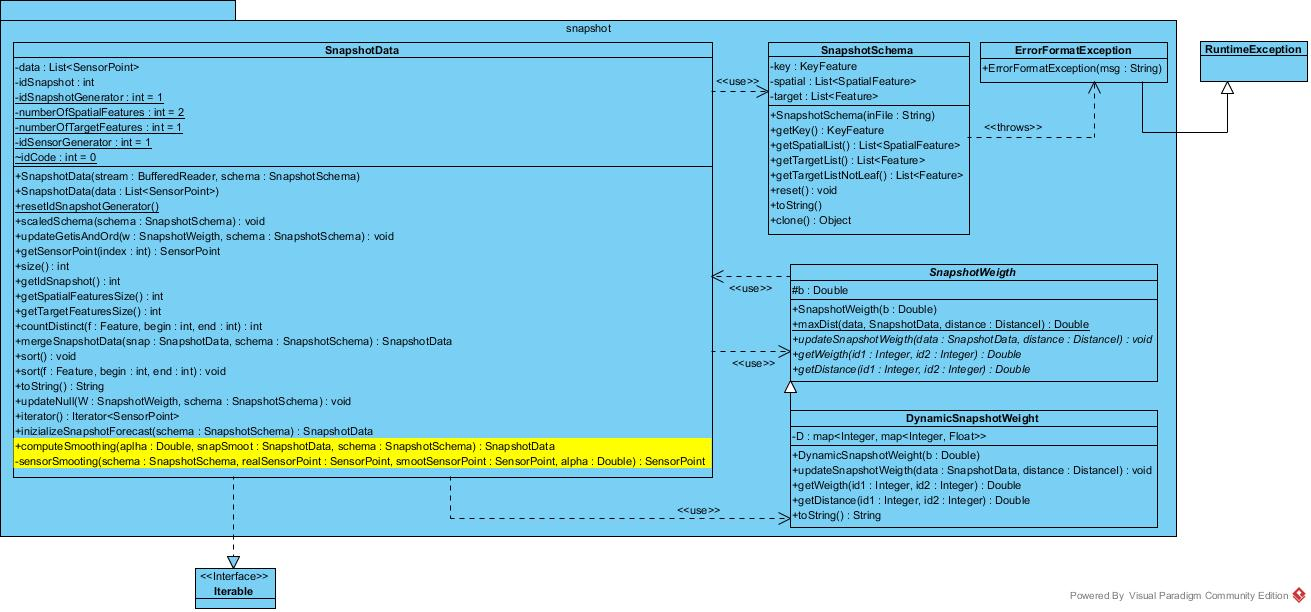
\includegraphics[width=449pt,height=\paperheight/2, angle = 90]{Smoothing/Snapshot_Class_Diagram.jpg}
\caption{Exponential Smoothing Class Diagram}
}
\label{ESCD}
\end{figure}
In Fig.~\ref{ESCD} sono presentate le modifiche apportate al package \textit{Snapshot}. 

Queste modifiche interessano la classe \textit{SnapshotData} e sono necessarie per modellare il meccanismo di smoothing esponenziale. 

Sono stati aggiunti due metodi, i quali ricevuto in input uno snapshot (quello sul quale è stato applicato il metodo di smoothing all'istante temporale precedente) si preoccupano di crearne uno nuovo, che è la fusione tra lo snapshot reale e quello in input. 

Tale snapshot è dato in input all'algoritmo di smoothing esponenziale.
\newpage
\begin{figure}[H]
\textbf{
\centering
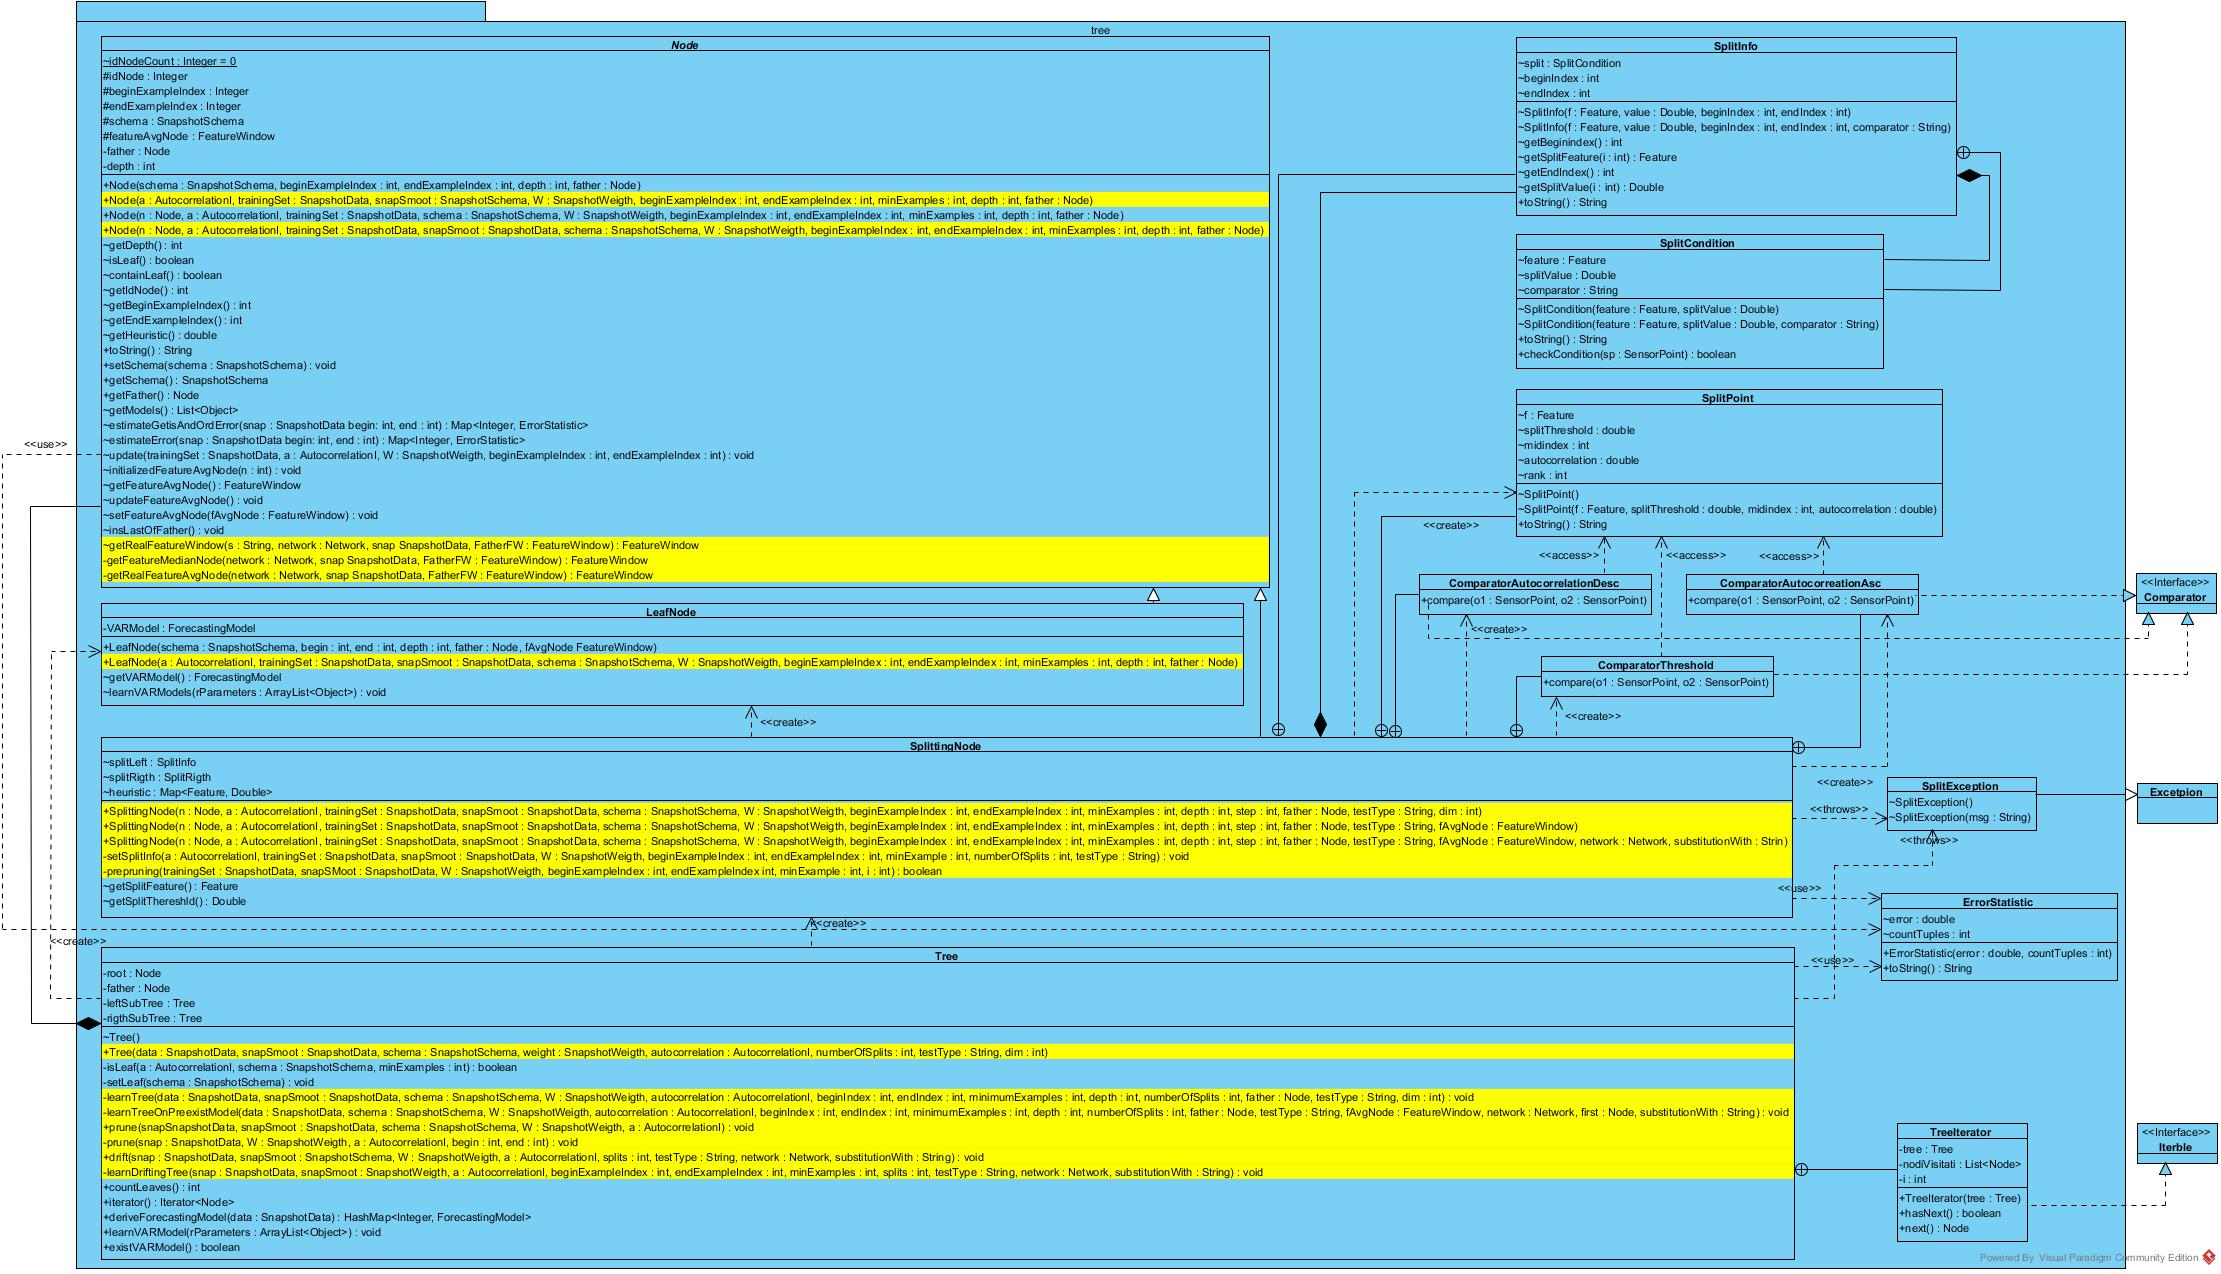
\includegraphics[width=\paperwidth,height=\paperheight/2, angle = 90]{Smoothing/Tree_Class_Diagram.jpg}
\caption{Tree Class Diagram VARForecaster 2.2}
}
\label{CTCD}
\end{figure}
\newpage
Quelle presentate in Fig.~\ref{CTCD} sono le modifiche al package \textit{Tree}. 

Dal momento che l'albero è costruito sulla base dei valori a cui è stato applicato lo smoothing esponenziale, si è resa necessaria la modifica della maggior parte delle firme dei metodi che si preoccupano della creazione dei vari nodi e dei metodi principali per la creazione del \textit{CT}.

\newpage
\subsubsection{Diagrammi di sequenza}
\begin{figure}[H]
\textbf{
\centering
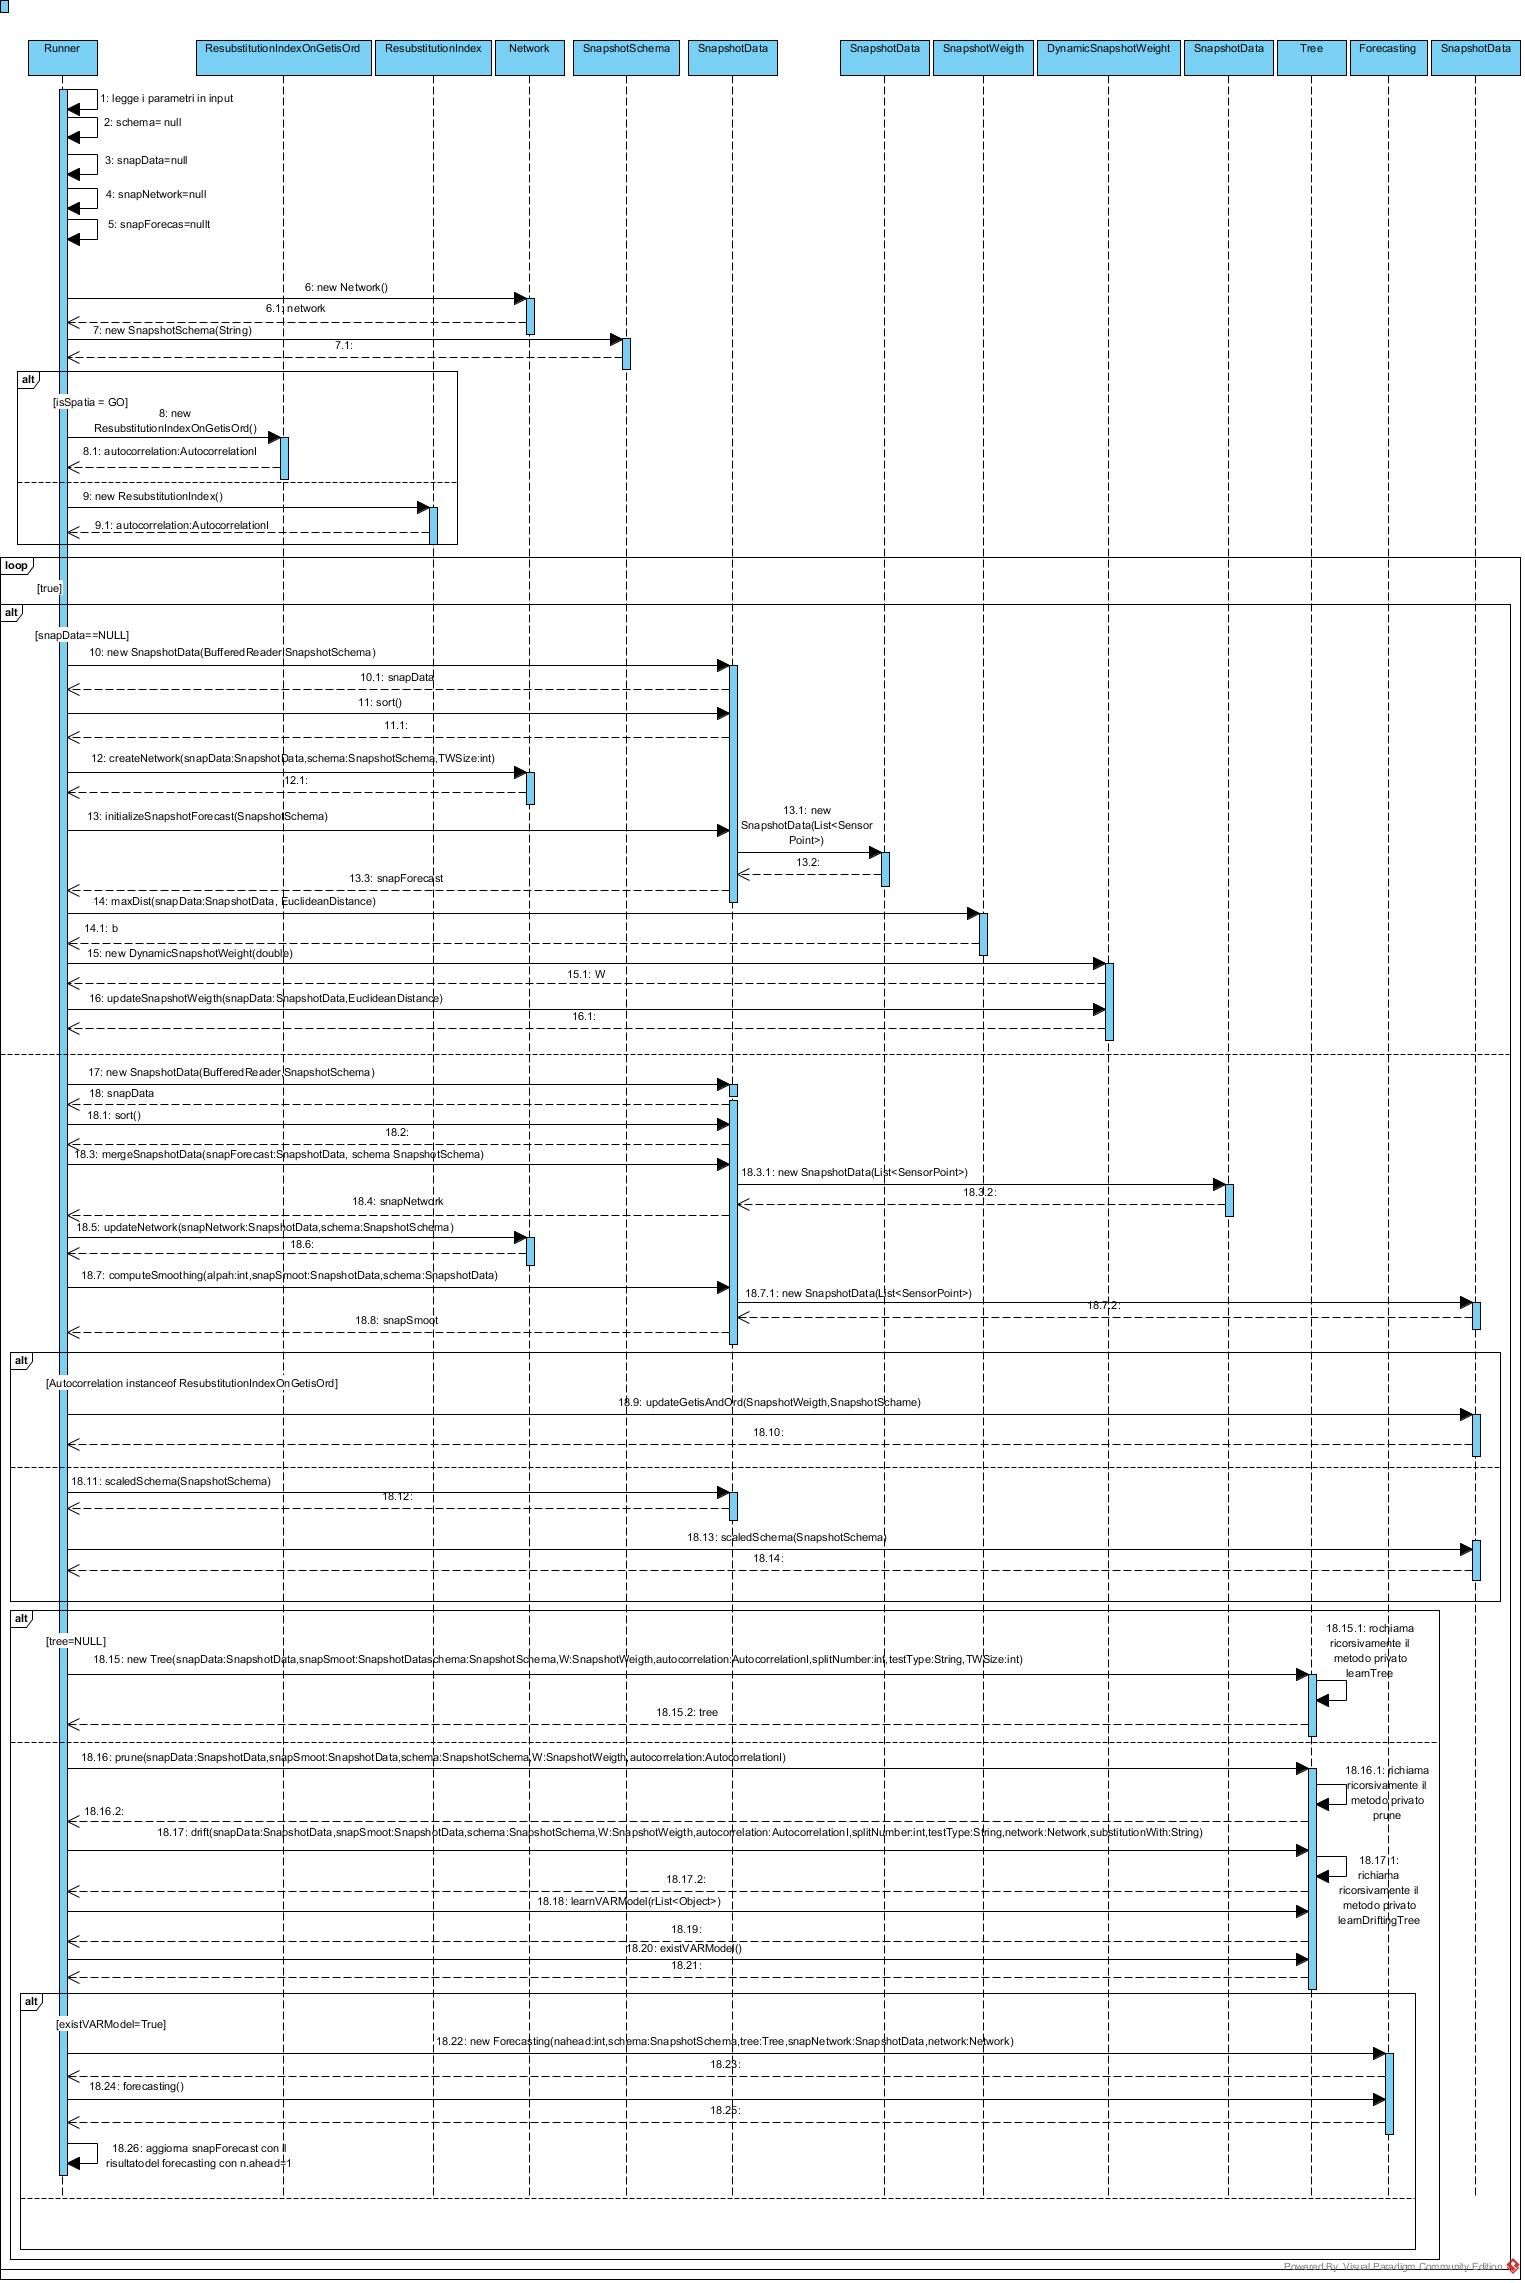
\includegraphics[width=0.8\textwidth]{Smoothing/run.jpg}
\caption{Run VARForecaster 2.2}
\label{run22}
}
\end{figure}
\newpage
\begin{figure}[H]
\textbf{
\centering
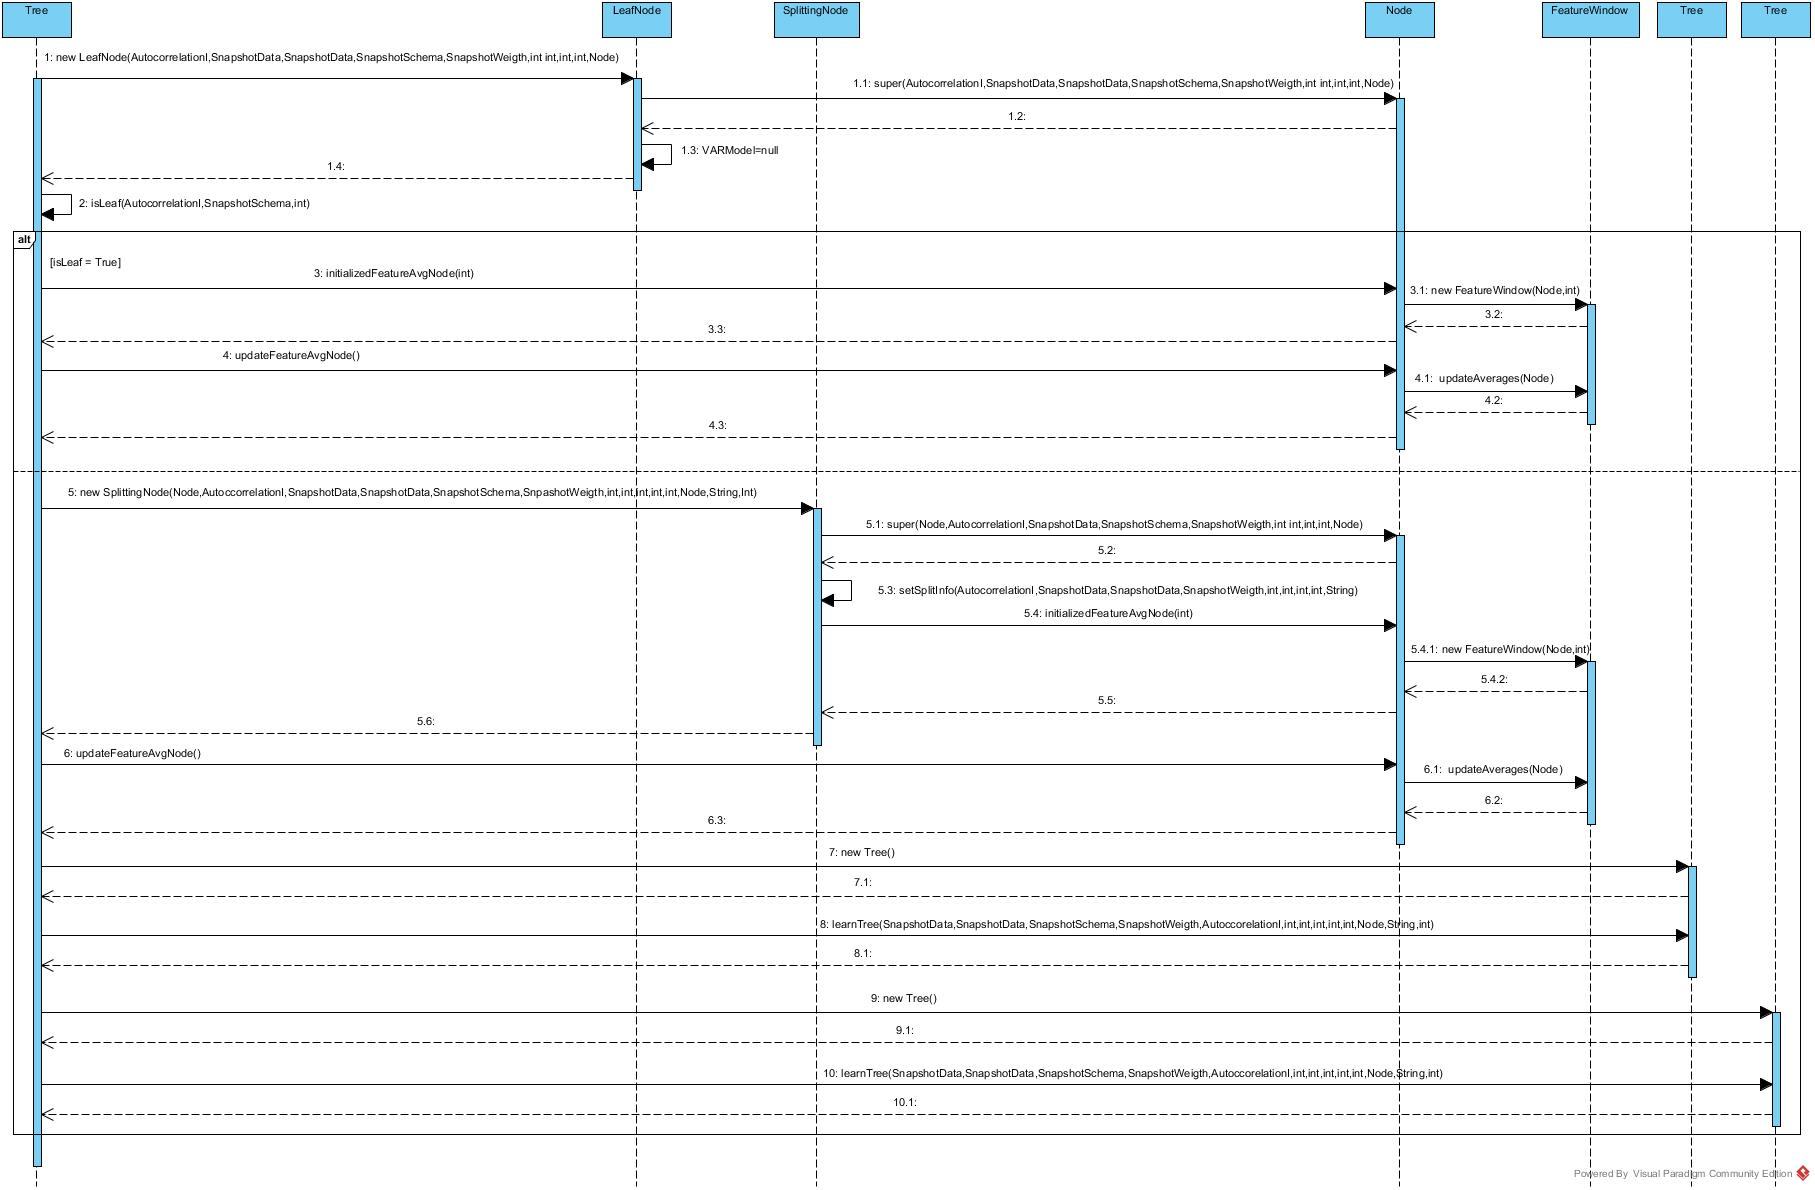
\includegraphics[width=\paperwidth,height=\paperheight/2, angle = 90]{Smoothing/learnCT.jpg}
\caption{Apprendimento CT VARForecaster 2.2}
\label{CT22}
}
\end{figure}
\newpage
\begin{figure}[H]
\textbf{
\centering
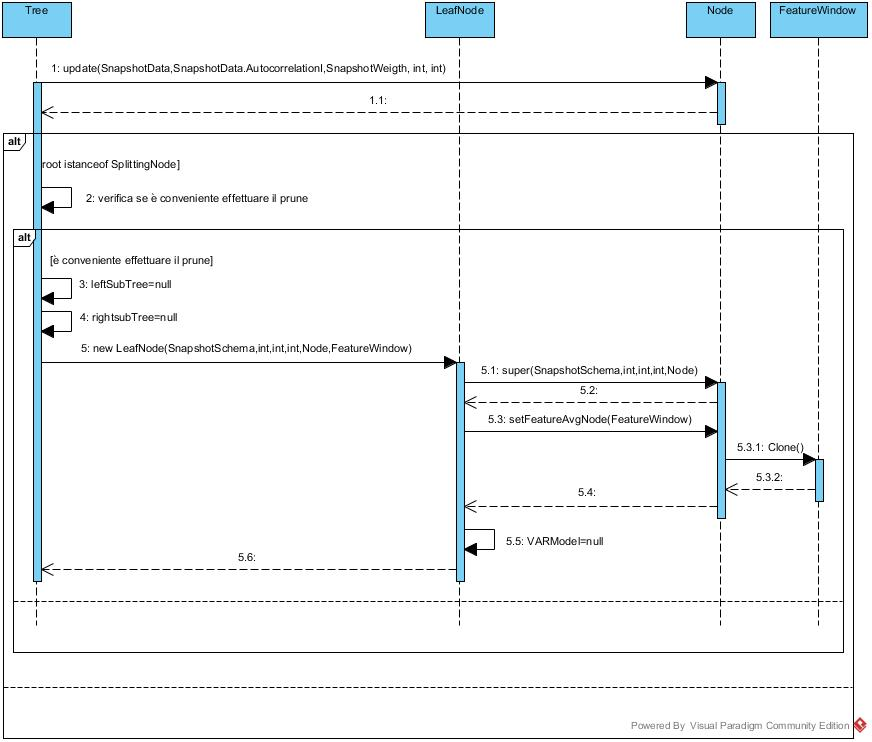
\includegraphics[width=0.8\textwidth]{Smoothing/prune.jpg}
\caption{Potatura VARForecaster 2.2}
\label{prune22}
}
\end{figure}
\newpage
\begin{figure}[H]
\textbf{
\centering
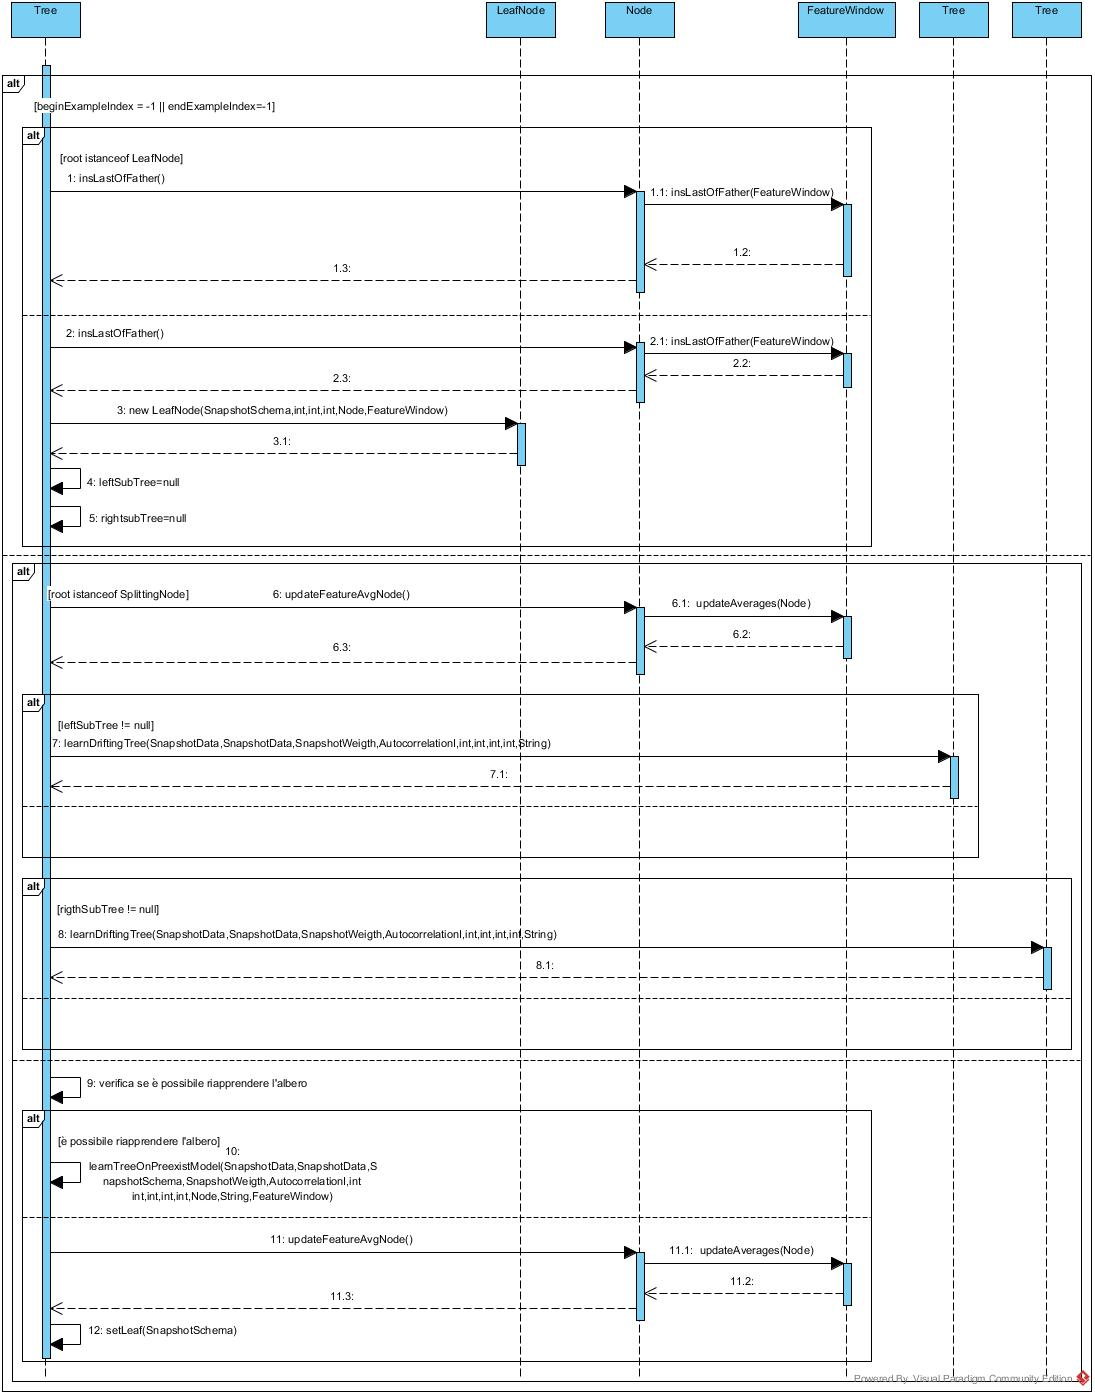
\includegraphics[width=0.8\textwidth]{Smoothing/drift.jpg}
\caption{Riapprendimento CT 1/2 VARForecaster 2.2}
\label{drift22}
}
\end{figure}
\newpage
\begin{figure}[H]
\textbf{
\centering
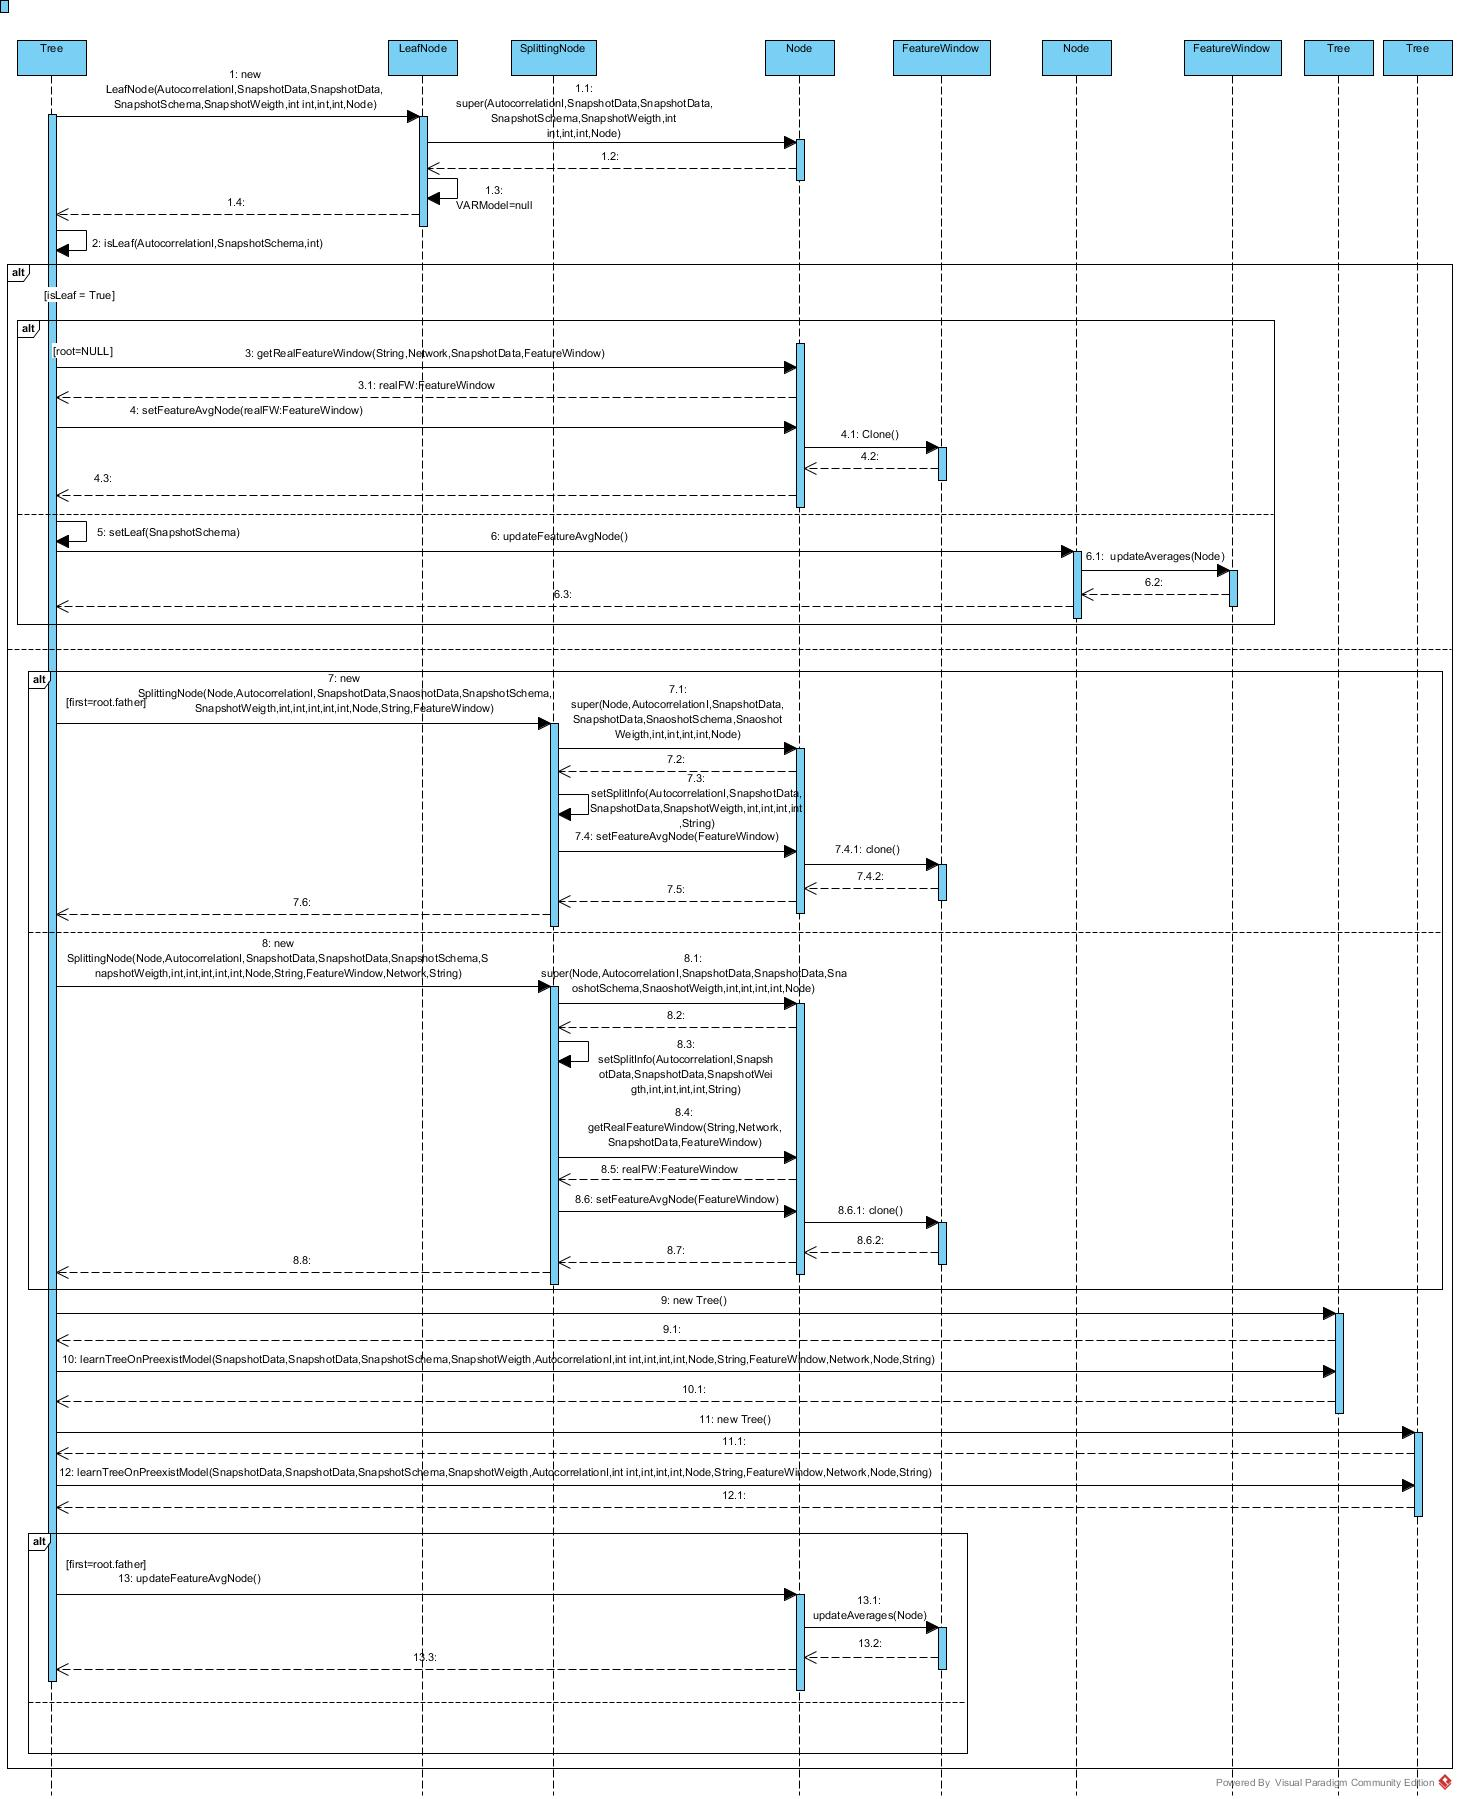
\includegraphics[width=\paperwidth,height=\paperheight/2, angle = 90]{Smoothing/learnTreeOnPreexistModel.jpg}
\caption{Riapprendimento CT 2/2 VARForecaster 2.2}
\label{LTOPM22}
}
\end{figure}
\newpage
\begin{figure}[H]
\textbf{
\centering
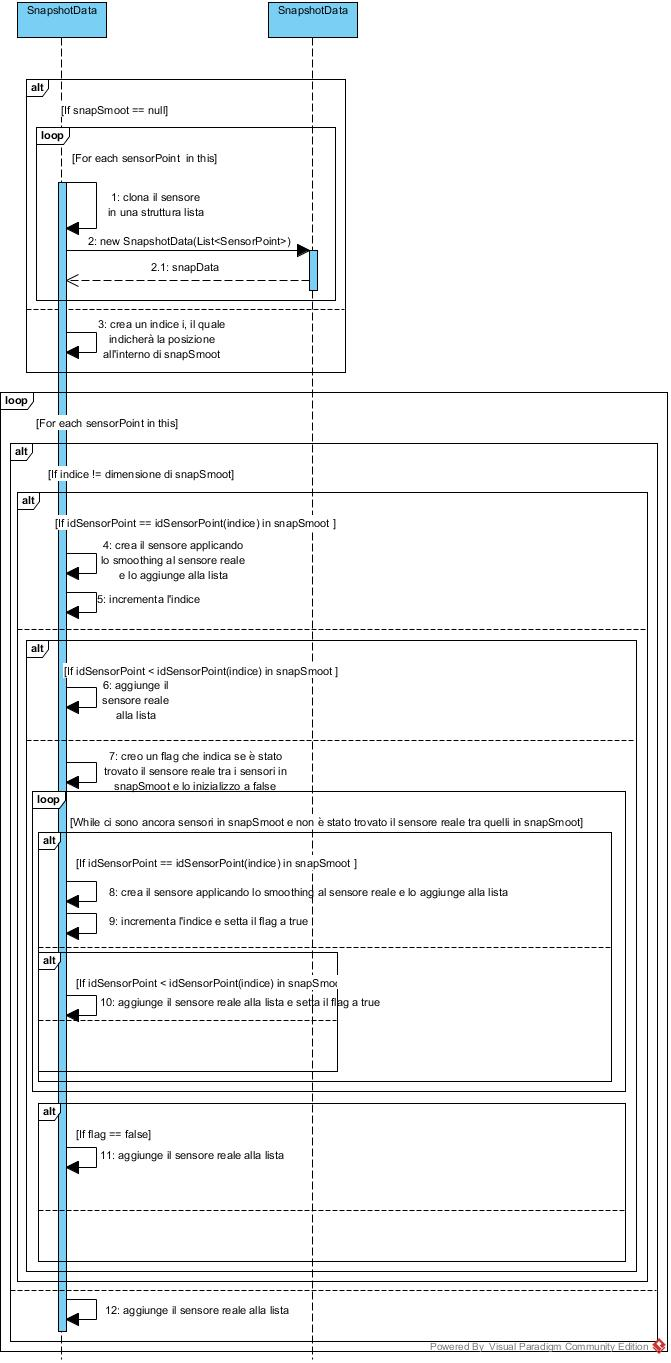
\includegraphics[width=0.8\textwidth]{Smoothing/computeSmoothing.jpg}
\caption{Algoritmo per lo smoothing esponenziale}
\label{CS22}
}
\end{figure}
\newpage
\begin{figure}[H]
\textbf{
\centering
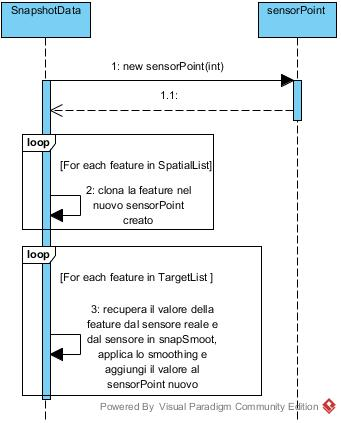
\includegraphics[width=0.8\textwidth]{Smoothing/sensorSmoothing.jpg}
\caption{Algoritmo per lo smoothing del singolo sensore}
\label{CSS22}
}
\end{figure}

\chapter{Analisi sperimentale}
In questa sezione sono descritti i risultati della valutazione empirica, condotta considerando due dataset di rilevazioni storiche. Questa valutazione è stata effettuata al fine di calcolare confrontare le prestazioni di VARForecaster 2.1 e VARForecaster 2.2, in termini di accuratezza della previsione ed efficienza della computazione.
\section{Obiettivi e metriche}
Si intende valutare:
\begin{itemize}
\item precisione nelle previsioni;
\item tempo di computazione necessario al completamento delle singole operazioni di costruzione(/riapprendimento) del \textit{CT}, apprendimento del modello VAR e previsione.
\end{itemize}
Tali obiettivi sono stati valutati mettendo a confronto i risultati ottenuti dalle sperimentazioni di \cite{donato} con quelle ottenute analizzando le versioni VARForecaster 2.1 e VARForecaster 2.2.

Al fine di valutare il raggiungimento di questi obiettivi sono state utilizzate le seguenti metriche:
\begin{enumerate}
\item Media dello RMSE per ogni istante di tempo predetto;
\item Deviazione standard dello RMSE per ogni istante di tempo predetto;
\item Numero di cluster generati dall'algoritmo di clustering in ogni istante di tempo;
\item Tempo medio di computazione per la costruzione(/riapprendimento) del \textit{CT};
\item Tempo medio di computazione per l'apprendimento del modello VAR;
\item Tempo medio di computazione per la fase di previsione.
\end{enumerate}
L'espressione matematica per il calcolo dello RMSE delle previsioni è:

$$RMSE_t = \sqrt{\frac{\sum_{i=1}^{n}{(\hat{y}_{(t,i)} - y_{(t,i)})^2}}{n}}$$

dove \textit{t} indica l'istante temporale in analisi e \textit{i} indica l'i-esimo sensore ed \textit{n} il numero totale di sensori.

Per la versione VARForecaster 2.1, non è stata utilizzata la metrica \textit{(3)} in quanto tale versione non implica alcuna variazione nell'algoritmo di clustering.

\newpage
\section{Dati}
Per le rilevazioni sono state utilizzate due reti di sensori:
\begin{itemize}
\item \textit{EcoTexas};
\item \textit{UnitedStatesPacific}.
\end{itemize} 
\textit{EcoTexas} è un dataset comprendente 26 sensori situati in Texas e i suoi attributi misurano: \textit{Temperatura}, \textit{velocità del vento}, \textit{livello di ozono}, \textit{livello di radiazioni solari}.

\textit{UnitedStatesPacific} invece è un dataset al cui interno ci sono le misurazioni di 190 sensori posizionati negli Stati Uniti d'America e in alcune isole del Pacifico. Queste rilevazioni riguardano: \textit{dewp}, \textit{pres}, \textit{temp}, \textit{wind}.

In entrambi i dataset sono effettuate rilevazioni a distanza di un ora una dall'altra e per ognuno di essi saranno considerati i primi 100 istanti temporali.
\newpage
\section{Risultati e discussione}
Sono di seguito elencati i risultati ottenuti in ottemperanza delle metriche scelte divisi in due sezioni, una per ogni dataset. 

Inizialmente si confrontano i risultati ottenuti utilizzando le diverse configurazioni del software realizzato. Tali risultati sono confrontati con i quelli riportati in \cite{donato}.
\subsection{Ecotexas}
Per il dataset Ecotexas sono stati utilizzati i seguenti parametri:

\begin{center}
\begin{table}[H]
\centering
\begin{tabular}{|c|c|}
\hline
\textbf{Dimensione finestra temporale} & 48 \\
\hline
\textbf{bperc.} & 0.1f \\
\hline
\textbf{lag.max} & 24 \\
\hline
\textbf{Season} & NULL \\
\hline
\textbf{Exogen} & NULL \\
\hline
\textbf{ic} & ALL \\
\hline
\textbf{type} & ALL \\
\hline
\textbf{n.ahead} & 6 \\
\hline
\end{tabular}
\caption{Parametri per Ecotexas}
\end{table}
\end{center}
dove "ALL" indica che è il sistema a trovare il parametro ottimale tra quelli ammissibili per la costruzione del modello VAR.

\medskip

\subsubsection{VARForecaster 2.1}

Nella versione VARForecaster 2.1 le configurazioni possibili sono:
\begin{enumerate}
\item Calcolo dell'aggregato con utilizzo della media e indice di autocorrelazione spaziale Getis and Ord;
\item Calcolo dell'aggregato con utilizzo della mediana e indice di autocorrelazione spaziale Getis and Ord;
\item Calcolo dell'aggregato con utilizzo della media e varianza;
\item Calcolo dell'aggregato con utilizzo della mediana e varianza;
\end{enumerate}

Per le metriche \textit{(1)} e \textit{(2)} (definite in Sezione 4.1) i risultati sono stati analizzati attributo per attributo e sono di seguito riportati.
\newpage
\textbf{Metrica 1: Media dello RMSE per ogni istante di tempo predetto} \medskip

Attributo: Temperatura \\ 
\begin{table}[H]
\centering
\begin{tabular}{|c|c|c|c|c|}
\hline
 & \textbf{Media+GO} & \textbf{Mediana+GO} & \textbf{Media+Var} & \textbf{Mediana+Var} \\
\hline
\textbf{ahead 1} & 7,727963 & 7,948522 & \textbf{6,872338} & 8,979301 \\
\hline
\textbf{ahead 2} & 12,11254 & 11,49216 & \textbf{10,90933} & 10,90759 \\
\hline
\textbf{ahead 3} & 14,88549 & 13,85234 & 14,0107 & \textbf{13,63754} \\
\hline
\textbf{ahead 4} & 16,50204 & \textbf{14,87442} & 17,18551 & 15,50205 \\
\hline
\textbf{ahead 5} & 17,89753 & \textbf{15,52931} & 19,55695 & 17,20633 \\
\hline
\textbf{ahead 6} & 19,80448 & \textbf{16,64003} & 22,31437 & 18,81037 \\
\hline
\end{tabular} \\
\caption{Ecotexas VARForecaster 2.1 - Metrica \textit{(1)}, temperatura}
\end{table} 

\medskip

Attributo: Velocità del vento \\ 

\begin{table}[H]
\centering
\begin{tabular}{|c|c|c|c|c|}
\hline
 & \textbf{Media+GO} & \textbf{Mediana+GO} & \textbf{Media+Var} & \textbf{Mediana+Var} \\
\hline
\textbf{ahead 1} & 2,770909 & 3,04784 & \textbf{2,72581} & 3,282296 \\
\hline
\textbf{ahead 2} & 4,169788 & 4,121688 & \textbf{3,947481} & 4,3164 \\
\hline
\textbf{ahead 3} & 5,187269 & 5,153598 & \textbf{4,636164} & 6,193093 \\
\hline
\textbf{ahead 4} & 6,26087 & 5,828 & \textbf{5,452935} & 6,193093 \\
\hline
\textbf{ahead 5} & 7,165297 & \textbf{6,319675} & 6,445137 & 6,770449 \\
\hline
\textbf{ahead 6} & 7,529702 & \textbf{6,481377} & 6,870087 & 7,400426 \\
\hline
\end{tabular} \\
\caption{Ecotexas VARForecaster 2.1 - Metrica \textit{(1)}, velocità del vento}
\end{table}

\medskip

Attributo:Ozono \\ 

\begin{table}[H]
\centering
\begin{tabular}{|c|c|c|c|c|}
\hline
 & \textbf{Media+GO} & \textbf{Mediana+GO} & \textbf{Media+Var} & \textbf{Mediana+Var} \\
\hline
\textbf{ahead 1} & \textbf{2,238133} & 2,427748 & 2,40774 & 2,583126 \\
\hline
\textbf{ahead 2} & \textbf{4,243109} & 4,385498 & 4,698071 & 4,492118 \\
\hline
\textbf{ahead 3} & \textbf{6,156216} & 6,199482 & 7,354431 & 6,490697 \\
\hline
\textbf{ahead 4} & 7,911378 & \textbf{7,752754} & 9,885487 & 8,301946 \\
\hline
\textbf{ahead 5} & 9,570941 & \textbf{8,988501} & 12,61612 & 10,03399 \\
\hline
\textbf{ahead 6} & 10,9282 & \textbf{9,906673} & 15,1254 & 11,47112 \\
\hline
\end{tabular} \\
\caption{Ecotexas VARForecaster 2.1 - Metrica \textit{(1)}, Ozono}
\end{table}

\medskip

Attributo: Radiazioni solari \\ 

\begin{table}[H]
\centering
\begin{tabular}{|c|c|c|c|c|}
\hline
 & \textbf{Media+GO} & \textbf{Mediana+GO} & \textbf{Media+Var} & \textbf{Mediana+Var} \\
\hline
\textbf{ahead 1} & 0,286194 & \textbf{0,250383} & 0,273884 & 0,31357 \\
\hline
\textbf{ahead 2} & 0,526701 & \textbf{0,461626} & 0,514967 & 0,527801 \\
\hline
\textbf{ahead 3} & 0,70248 & \textbf{0,641239} & 0,741909 & 0,690238 \\
\hline
\textbf{ahead 4} & 0,827084 & \textbf{0,744024} & 0,901843 & 0,795779 \\
\hline
\textbf{ahead 5} & 0,910664 & \textbf{0,790287} & 1,098361 & 0,900938 \\
\hline
\textbf{ahead 6} & 0,987533 & \textbf{0,808239} & 1,274128 & 0,97393 \\
\hline
\end{tabular}
\caption{Ecotexas VARForecaster 2.1 - Metrica \textit{(1)}, radiazioni solari}
\end{table}
\newpage

\textbf{Metrica 2: Deviazione standard dello RMSE per ogni istante di tempo predetto}

\medskip


Attributo: Temperatura \\

\begin{table}[H]
\centering
\begin{tabular}{|c|c|c|c|c|}
\hline
 & \textbf{Media+GO} & \textbf{Mediana+GO} & \textbf{Media+Var} & \textbf{Mediana+Var} \\
\hline
\textbf{ahead 1} & 3,263198 & 2,529772 & \textbf{1,565324} & 4,585758 \\
\hline
\textbf{ahead 2} & 5,858031 & 3,811666 & 2,713763 & \textbf{2,085918} \\
\hline
\textbf{ahead 3} & 7,294031 & 4,746114 & \textbf{3,654802} & 3,949568 \\
\hline
\textbf{ahead 4} & 7,876128 & 5,066172 & \textbf{4,780009} & 5,32213 \\
\hline
\textbf{ahead 5} & 9,245492 & 6,327062 & \textbf{5,223495} & 6,933482 \\
\hline
\textbf{ahead 6} & 12,30531 & \textbf{7,596333} & 10,00537 & 8,577916 \\
\hline
\end{tabular} \\
\caption{Ecotexas VARForecaster 2.1 - Metrica \textit{(2)}, temperatura}
\end{table}

\medskip

Attributo: Velocità del vento \\ 

\begin{table}[H]
\centering
\begin{tabular}{|c|c|c|c|c|}
\hline
 & \textbf{Media+GO} & \textbf{Mediana+GO} & \textbf{Media+Var} & \textbf{Mediana+Var} \\
\hline
\textbf{ahead 1} & 0,751254 & 1,051378 & \textbf{0,661512} & 1,301704 \\
\hline
\textbf{ahead 2} & 1,227334 & 1,340969 & \textbf{1,030355} & 1,183548 \\
\hline
\textbf{ahead 3} & 1,630038 & 1,661901 & \textbf{1,043562} & 1,718451 \\
\hline
\textbf{ahead 4} & 2,449047 & 1,859191 & \textbf{1,442913} & 2,132098 \\
\hline
\textbf{ahead 5} & 3,067828 & 2,258222 & \textbf{2,172139} & 2,589733 \\
\hline
\textbf{ahead 6} & 3,766907 & \textbf{2,412196} & 2,687215 & 2,957897 \\
\hline
\end{tabular} \\
\caption{Ecotexas VARForecaster 2.1 - Metrica \textit{(2)}, Velocità del vento}
\end{table}

\medskip

Attributo: Ozono \\ 

\begin{table}[H]
\centering
\begin{tabular}{|c|c|c|c|c|}
\hline
 & \textbf{Media+GO} & \textbf{Mediana+GO} & \textbf{Media+Var} & \textbf{Mediana+Var} \\
\hline
\textbf{ahead 1} & 1,327452 & \textbf{0,704212} & 1,126675 & 1,251867 \\
\hline
\textbf{ahead 2} & 2,076686 & \textbf{1,055576} & 1,566866 & 1,709158 \\
\hline
\textbf{ahead 3} & 2,125811 & \textbf{1,487432} & 3,604166 & 2,261353 \\
\hline
\textbf{ahead 4} & 2,317416 & \textbf{2,047489} & 5,101176 & 2,745594 \\
\hline
\textbf{ahead 5} & \textbf{2,75666} & 2,833415 & 11,58965 & 3,986299 \\
\hline
\textbf{ahead 6} & \textbf{3,687823} & 3,706639 & 19,3885 & 5,149975 \\
\hline
\end{tabular} \\
\caption{Ecotexas VARForecaster 2.1 - Metrica \textit{(2)}, Ozono}
\end{table}

\medskip

Attributo: Radiazioni solari \\ 

\begin{table}[H]
\centering
\begin{tabular}{|c|c|c|c|c|}
\hline
 & \textbf{Media+GO} & \textbf{Mediana+GO} & \textbf{Media+Var} & \textbf{Mediana+Var} \\
\hline
\textbf{ahead 1} & 0,090172 & 0,097816 & \textbf{0,073123} & 0,101597 \\
\hline
\textbf{ahead 2} & 0,175438 & 0,198805 & \textbf{0,129505} & 0,162625 \\
\hline
\textbf{ahead 3} & 0,24637 & 0,293015 & 0,286108 & \textbf{0,210677} \\
\hline
\textbf{ahead 4} & 0,307636 & 0,341056 & 0,394155 & \textbf{0,266356} \\
\hline
\textbf{ahead 5} & 0,346291 & \textbf{0,342398} & 0,950618 & 0,357383 \\
\hline
\textbf{ahead 6} & 0,433747 & \textbf{0,097816} & 1,41983 & 0,396003 \\
\hline
\end{tabular} 
\caption{Ecotexas VARForecaster 2.1 - Metrica \textit{(2)}, radiazioni solari}
\end{table}
\newpage
Per entrambe le metriche sono riportati in \textbf{grassetto} gli RMSE più bassi ottenuti per ogni istante temporale previsto. 

Per meglio comprendere questi risultati si riportano nel seguito le tabelle, una per ogni istante di tempo di previsione (ahead), riportanti il numero di volte che una configurazione è stata scelta come migliore.

\medskip
\textbf{Ahead = 1}


\begin{table}[H]
\centering
\begin{tabular}{|c|c|c|c|c|c|c|c|c|c|c|c|c|}
\hline
 & \multicolumn{4}{|c|}{\textbf{Totale}} & \multicolumn{4}{|c|}{\textbf{Metrica 1}} & \multicolumn{4}{|c|}{\textbf{Metrica 2}} \\
\hline
\textbf{Configurazioni} & 1 & 2 & \textbf{3} & 4 & 1 & 2 & 3 & 4 & 1 & 2 & 3 & 4 \\
\hline
\textbf{Occorrenze} & 1 & 2 & \textbf{5} & 0 & 1 & 1 & 2 & 0 & 0 & 1 & 3 & 0\\
\hline
\end{tabular}
\caption{Ecotexas VARForecaster 2.1 - Riassunto Ahead 1}
\end{table}

\medskip
\textbf{Ahead = 2}


\begin{table}[H]
\centering
\begin{tabular}{|c|c|c|c|c|c|c|c|c|c|c|c|c|}
\hline
 & \multicolumn{4}{|c|}{\textbf{Totale}} & \multicolumn{4}{|c|}{\textbf{Metrica 1}} & \multicolumn{4}{|c|}{\textbf{Metrica 2}} \\
\hline
\textbf{Configurazioni} & 1 & 2 & \textbf{3} & 4 & 1 & 2 & 3 & 4 & 1 & 2 & 3 & 4 \\
\hline
\textbf{Occorrenze} & 1 & 2 & \textbf{4} & 1 & 1 & 1 & 2 & 0 & 0 & 1 & 2 & 1\\
\hline
\end{tabular}
\caption{Ecotexas VARForecaster 2.1 - Riassunto Ahead 2}
\end{table}

\medskip
\textbf{Ahead = 3}


\begin{table}[H]
\centering
\begin{tabular}{|c|c|c|c|c|c|c|c|c|c|c|c|c|}
\hline
 & \multicolumn{4}{|c|}{\textbf{Totale}} & \multicolumn{4}{|c|}{\textbf{Metrica 1}} & \multicolumn{4}{|c|}{\textbf{Metrica 2}} \\
\hline
\textbf{Configurazioni} & 1 & 2 & \textbf{3} & 4 & 1 & 2 & 3 & 4 & 1 & 2 & 3 & 4 \\
\hline
\textbf{Occorrenze} & 1 & 2 & \textbf{3} & 2 & 1 & 1 & 1 & 1 & 0 & 1 & 2 & 1\\
\hline
\end{tabular}
\caption{Ecotexas VARForecaster 2.1 - Riassunto Ahead 3}
\end{table}

\medskip
\textbf{Ahead = 4}


\begin{table}[H]
\centering
\begin{tabular}{|c|c|c|c|c|c|c|c|c|c|c|c|c|}
\hline
 & \multicolumn{4}{|c|}{\textbf{Totale}} & \multicolumn{4}{|c|}{\textbf{Metrica 1}} & \multicolumn{4}{|c|}{\textbf{Metrica 2}} \\
\hline
\textbf{Configurazioni} & 1 & \textbf{2} & 3 & 4 & 1 & 2 & 3 & 4 & 1 & 2 & 3 & 4 \\
\hline
\textbf{Occorrenze} & 0 & \textbf{4} & 3 & 1 & 0 & 3 & 1 & 0 & 0 & 1 & 2 & 1\\
\hline
\end{tabular}
\caption{Ecotexas VARForecaster 2.1 - Riassunto Ahead 4}
\end{table}

\medskip
\textbf{Ahead = 5}


\begin{table}[H]
\centering
\begin{tabular}{|c|c|c|c|c|c|c|c|c|c|c|c|c|}
\hline
 & \multicolumn{4}{|c|}{\textbf{Totale}} & \multicolumn{4}{|c|}{\textbf{Metrica 1}} & \multicolumn{4}{|c|}{\textbf{Metrica 2}} \\
\hline
\textbf{Configurazioni} & 1 & \textbf{2} & 3 & 4 & 1 & 2 & 3 & 4 & 1 & 2 & 3 & 4 \\
\hline
\textbf{Occorrenze} & 1 & \textbf{5} & 2 & 0 & 1 & 4 & 0 & 0 & 1 & 1 & 2 & 0\\
\hline
\end{tabular}
\caption{Ecotexas VARForecaster 2.1 - Riassunto Ahead 5}
\end{table}

\medskip
\textbf{Ahead = 6}


\begin{table}[H]
\centering
\begin{tabular}{|c|c|c|c|c|c|c|c|c|c|c|c|c|}
\hline
 & \multicolumn{4}{|c|}{\textbf{Totale}} & \multicolumn{4}{|c|}{\textbf{Metrica 1}} & \multicolumn{4}{|c|}{\textbf{Metrica 2}} \\
\hline
\textbf{Configurazioni} & 1 & \textbf{2} & 3 & 4 & 1 & 2 & 3 & 4 & 1 & 2 & 3 & 4 \\
\hline
\textbf{Occorrenze} & 1 & \textbf{7} & 0 & 0 & 0 & 4 & 0 & 0 & 1 & 3 & 0 & 0\\
\hline
\end{tabular}
\caption{Ecotexas VARForecaster 2.1 - Riassunto Ahead 6}
\end{table} 

\medskip

Si noti che, in base alle metriche \textit{(1)} e \textit{(2)}, utilizzate per valutare l'accuratezza di VARForecaster 2.1, la configurazione migliore per le prime 3 previsioni è la \textit{3}, nonché il calcolo dell'aggregato con uso di media e la varianza, mentre per le successive è di gran lunga migliore la configurazione \textit{2}, ovvero il calcolo dell'aggregato con l'utilizzo della mediana e indice di autocorrelazione spaziale Getis and Ord.

\medskip

\textbf{Metrica 4: Tempo medio di computazione per la costruzione(/riapprendimento) del \textit{CT}.}

\medskip


\begin{table}[H]
\centering
\begin{tabular}[H]{|c|c|c|c|}
\hline
\textbf{Media+GO} & \textbf{Mediana+GO} & \textbf{Media+Var} & \textbf{Mediana+Var} \\
\hline
4,43 & 3,67 & 4,20 & \textbf{3,36} \\
\hline
\end{tabular}
\caption{Ecotexas VARForecaster 2.1 - Metrica \textit{(4)}}
\end{table} 

\medskip 
\textbf{Metrica 5: Tempo medio di computazione per l'apprendimento del modello VAR.}

\medskip

\begin{table}[H]
\centering
\begin{tabular}[H]{|c|c|c|c|}
\hline
\textbf{Media+GO} & \textbf{Mediana+GO} & \textbf{Media+Var} & \textbf{Mediana+Var} \\
\hline
\textbf{6782} & \textbf{6782} & 7314 & 7299 \\
\hline
\end{tabular}
\caption{Ecotexas VARForecaster 2.1 - Metrica \textit{(5)}}
\end{table} 

\medskip 
\textbf{Metrica 6: Tempo medio di computazione per la fase di previsione.}

\medskip


\begin{table}[H]
\centering
\begin{tabular}[H]{|c|c|c|c|}
\hline
\textbf{Media+GO} & \textbf{Mediana+GO} & \textbf{Media+Var} & \textbf{Mediana+Var} \\
\hline
1,59 & \textbf{1,30} & 1,60 & 1,88 \\
\hline
\end{tabular}
\caption{Ecotexas VARForecaster 2.1 - Metrica \textit{(6)}}
\end{table} 

\newpage
\subsubsection{VARForecaster 2.2}


Per la versione VARForecaster 2.2 le configurazioni possibili sono:
\begin{enumerate}
\item Apprendimento dell'albero con algoritmo di smoothing utilizzando un $ \alpha = 0.4$, calcolo dell'aggregato con la mediana e indice di autocorrelazione spaziale Getis and Ord.
\item Apprendimento dell'albero con algoritmo di smoothing utilizzando un $ \alpha = 0.4$, calcolo dell'aggregato con la media e indice di autocorrelazione spaziale Getis and Ord.
\item Apprendimento dell'albero con algoritmo di smoothing utilizzando un $ \alpha = 0.4$, calcolo dell'aggregato con la mediana e varianza.
\item Apprendimento dell'albero con algoritmo di smoothing utilizzando un $ \alpha = 0.4$, calcolo dell'aggregato con la media e varianza.
\item Apprendimento dell'albero con algoritmo di smoothing utilizzando un $ \alpha = 0.5$, calcolo dell'aggregato con la mediana e indice di autocorrelazione spaziale Getis and Ord.
\item Apprendimento dell'albero con algoritmo di smoothing utilizzando un $ \alpha = 0.5$, calcolo dell'aggregato con la media e indice di autocorrelazione spaziale Getis and Ord.
\item Apprendimento dell'albero con algoritmo di smoothing utilizzando un $ \alpha = 0.5$, calcolo dell'aggregato con la mediana e varianza.
\item Apprendimento dell'albero con algoritmo di smoothing utilizzando un $ \alpha = 0.5$, calcolo dell'aggregato con la media e varianza.
\item Apprendimento dell'albero con algoritmo di smoothing utilizzando un $ \alpha = 0.6$, calcolo dell'aggregato con la mediana e indice di autocorrelazione spaziale Getis and Ord.
\item Apprendimento dell'albero con algoritmo di smoothing utilizzando un $ \alpha = 0.6$, calcolo dell'aggregato con la media e indice di autocorrelazione spaziale Getis and Ord.
\item Apprendimento dell'albero con algoritmo di smoothing utilizzando un $ \alpha = 0.6$, calcolo dell'aggregato con la mediana e varianza.
\item Apprendimento dell'albero con algoritmo di smoothing utilizzando un $ \alpha = 0.6$, calcolo dell'aggregato con la media e varianza.
\end{enumerate}

Per le metriche \textit{(1)} e \textit{(2)} i risultati sono stati analizzati attributo per attributo. Le tabelle sono organizzate in base ai livelli $\alpha$ Ogni tabella, inoltre, include le seguenti quattro colonne:

\begin{enumerate}
\item Calcolo dell'aggregato con utilizzo della mediana e indice di autocorrelazione spaziale Getis and Ord;
\item Calcolo dell'aggregato con utilizzo della media e indice di autocorrelazione spaziale Getis and Ord;
\item Calcolo dell'aggregato con utilizzo della mediana e varianza;
\item Calcolo dell'aggregato con utilizzo della media e varianza;
\end{enumerate}

Sono di seguito riportati i risultati.

\medskip

\textbf{Metrica 1: Media dello RMSE per ogni istante di tempo predetto} \medskip

Attributo: Temperatura \\ 

\begin{table}[H]
\centering
\begin{tabular}{|c|c|c|c|c|}
\hline
 & \multicolumn{4}{|c|}{Smoothing $\alpha$ = 0.4} \\
\hline
& 1 & 2 & 3 & 4 \\
\hline
\textbf{ahead 1} & 9,02206 & 8,483192 & 9,617287 & 9,230679\\
\hline
\textbf{ahead 2} & \textbf{11,74263} & 12,83586 & 12,1994 & 13,47861\\ 
\hline
\textbf{ahead 3} & \textbf{13,42569} & 14,90105 & 13,57288 & 16,27871\\
\hline
\textbf{ahead 4} & 14,68293 & 17,28901 & 15,09509 & 19,3797\\ 
\hline
\textbf{ahead 5} & 15,70545 & 19,53582 & 16,34737 & 22,68712\\
\hline
\textbf{ahead 6} & 16,76946 & 20,35719 & 17,25566 & 26,72587\\ 
\hline
\end{tabular} \\
\caption{Ecotexas VARForecaster 2.2 - Metrica \textit{(1)}, temperatura, $\alpha$ = 0.4}
\end{table} 

\newpage

\begin{table}[H]
\centering
\begin{tabular}{|c|c|c|c|c|}
\hline
 & \multicolumn{4}{|c|}{Smoothing $\alpha$ = 0.5} \\
\hline
& 1 & 2 & 3 & 4 \\
\hline
\textbf{ahead 1} & 9,03935 & \textbf{7,755912} & 9,272419 & 8,858649\\
\hline
\textbf{ahead 2} & 12,0037 & 12,59115 & 13,35981 & 14,01498\\ 
\hline
\textbf{ahead 3} & 13,53915 & 15,10238 & 15,57883 & 16,76933\\
\hline
\textbf{ahead 4} & \textbf{14,42594} & 16,811218 & 17,08853 & 18,59352\\ 
\hline
\textbf{ahead 5} & \textbf{15,03058} & 17,7564 & 18,48882 & 20,60122\\
\hline
\textbf{ahead 6} & \textbf{15,5948} & 18,30791 & 18,95518 & 21,3973\\ 
\hline
\end{tabular} \\
\caption{Ecotexas VARForecaster 2.2 - Metrica \textit{(1)}, temperatura, $\alpha$ = 0.5}
\end{table} 

\medskip

\begin{table}[H]
\centering
\begin{tabular}{|c|c|c|c|c|}
\hline
 & \multicolumn{4}{|c|}{Smoothing $\alpha$ = 0.6} \\
\hline
& 1 & 2 & 3 & 4 \\
\hline
\textbf{ahead 1} & 9,051656 & 7,845343 & 8,4815551 & 7,983976\\
\hline
\textbf{ahead 2} & 12,28307 & 12,52572 & 12,01534 & 13,06673\\ 
\hline
\textbf{ahead 3} & 14,20874 &  14,86637&  14,34806& 16,98019\\
\hline
\textbf{ahead 4} & 15,45715 & 15,9518 & 15,92537 & 19,46083\\ 
\hline
\textbf{ahead 5} & 15,73302 & 17,83478 & 17,25861 & 21,5627\\
\hline
\textbf{ahead 6} & 15,81711 & 18,77403 & 18,09892 & 24,41888\\ 
\hline
\end{tabular} \\
\caption{Ecotexas VARForecaster 2.2 - Metrica \textit{(1)}, temperatura, $\alpha$ = 0.6}
\end{table} 

\medskip

Attributo: Velocità del vento \\ 

\begin{table}[H]
\centering
\begin{tabular}{|c|c|c|c|c|}
\hline
 & \multicolumn{4}{|c|}{Smoothing $\alpha$ = 0.4} \\
\hline
& 1 & 2 & 3 & 4 \\
\hline
\textbf{ahead 1} & 3,01268 & 2,893663 & 3,394852 & 3,3447959\\
\hline
\textbf{ahead 2} & 4,143725 & 4,007819 & 4,041859 & 4,655479\\ 
\hline
\textbf{ahead 3} & 4,952245 & 4,943684 & \textbf{4,731441} & 6,191785\\
\hline
\textbf{ahead 4} &  5,620227& 5,758045 & 5,506629 & 9,587068\\ 
\hline
\textbf{ahead 5} & 6,061869 & 6,266921 & 6,224269 & 12,80314\\
\hline
\textbf{ahead 6} & 6,167213 & 6,426425 & 6,634878 & 22,5346\\ 
\hline
\end{tabular} \\
\caption{Ecotexas VARForecaster 2.2 - Metrica \textit{(1)}, velocità del vento, $\alpha$ = 0.4}
\end{table} 

\medskip

\begin{table}[H]
\centering
\begin{tabular}{|c|c|c|c|c|}
\hline
 & \multicolumn{4}{|c|}{Smoothing $\alpha$ = 0.5} \\
\hline
& 1 & 2 & 3 & 4 \\
\hline
\textbf{ahead 1} & 2,9068 & 2,719515 & 3,514897 & 3,439094\\
\hline
\textbf{ahead 2} & 4,247564 & 3,955123 & 4,631042 & 4,101132\\ 
\hline
\textbf{ahead 3} & 5,137302 & 4,920545 & 5,501999 & 5,38875\\
\hline
\textbf{ahead 4} & 5,90867 & 5,900318 & 6,819834 & 6,490254\\ 
\hline
\textbf{ahead 5} & 6,590004 & 6,487704 & 7,331173 & 7,12788\\
\hline
\textbf{ahead 6} & 7,022727 & 6,948599 & 7,694757 & 8,925594\\ 
\hline
\end{tabular} \\
\caption{Ecotexas VARForecaster 2.2 - Metrica \textit{(1)}, velocità del vento, $\alpha$ = 0.5}
\end{table} 

\medskip

\begin{table}[H]
\centering
\begin{tabular}{|c|c|c|c|c|}
\hline
 & \multicolumn{4}{|c|}{Smoothing $\alpha$ = 0.6} \\
\hline
& 1 & 2 & 3 & 4 \\
\hline
\textbf{ahead 1} & 2,964297 & \textbf{2,690527} & 3,181186 & 2,892368\\
\hline
\textbf{ahead 2} & 4,22764 & \textbf{3,851252} & 4,287462 & 4,237999\\ 
\hline
\textbf{ahead 3} & 5,140163 & 4,794959 & 5,434163 & 5,169286\\
\hline
\textbf{ahead 4} & 5,646351 & \textbf{5,481132} & 6,529889 & 6,104721\\ 
\hline
\textbf{ahead 5} & 5,952523 & \textbf{5,89235} & 7,077656 & 7,057257\\
\hline
\textbf{ahead 6} &  \textbf{6,099744}& 6,495151 & 7,710398 & 8,019449\\ 
\hline
\end{tabular} \\
\caption{Ecotexas VARForecaster 2.2 - Metrica \textit{(1)}, velocità del vento, $\alpha$ = 0.6}
\end{table} 

\medskip

Attributo:Ozono \\ 

\begin{table}[H]
\centering
\begin{tabular}{|c|c|c|c|c|}
\hline
 & \multicolumn{4}{|c|}{Smoothing $\alpha$ = 0.4} \\
\hline
& 1 & 2 & 3 & 4 \\
\hline
\textbf{ahead 1} & 2,841519 & 2,457334 & 2,727729 & \textbf{2,410487}\\
\hline
\textbf{ahead 2} & 5,139587 & 4,746671 & 4,568687 & 4,689119\\ 
\hline
\textbf{ahead 3} & 7,034836 & 7,497044 & 6,303611 & 6,795089\\
\hline
\textbf{ahead 4} & 8,55406 & 9,42643 & 8,218017 & 9,785377\\ 
\hline
\textbf{ahead 5} & 10,0661 & 10,82114 & 9,935751 & 13,15565\\
\hline
\textbf{ahead 6} & 10,91466 & 11,64655 & 11,27033 & 16,05161\\ 
\hline
\end{tabular} \\
\caption{Ecotexas VARForecaster 2.2 - Metrica \textit{(1)}, ozono, $\alpha$ = 0.4}
\end{table} 

\medskip

\begin{table}[H]
\centering
\begin{tabular}{|c|c|c|c|c|}
\hline
 & \multicolumn{4}{|c|}{Smoothing $\alpha$ = 0.5} \\
\hline
& 1 & 2 & 3 & 4 \\
\hline
\textbf{ahead 1} & 2,537652 & 2,550679 & 2,538546 & 2,617726\\
\hline
\textbf{ahead 2} & \textbf{4,466039} & 4,762223 & 4,83846 & 5,324233\\ 
\hline
\textbf{ahead 3} & \textbf{6,182669} & 7,020338 & 6,818731 & 7,833455\\
\hline
\textbf{ahead 4} & \textbf{7,838081} & 8,945195 & 8,463908 & 10,06753\\ 
\hline
\textbf{ahead 5} & \textbf{9,002074} & 10,54354 & 10,01062 & 12,69932\\
\hline
\textbf{ahead 6} & \textbf{9,959309} & 11,5342 & 11,32749 & 14,90097\\ 
\hline
\end{tabular} \\
\caption{Ecotexas VARForecaster 2.2 - Metrica \textit{(1)}, ozono, $\alpha$ = 0.5}
\end{table} 

\medskip

\begin{table}[H]
\centering
\begin{tabular}{|c|c|c|c|c|}
\hline
 & \multicolumn{4}{|c|}{Smoothing $\alpha$ = 0.6} \\
\hline
& 1 & 2 & 3 & 4 \\
\hline
\textbf{ahead 1} & 3,046583 & 2,579972 & 2,631889 & 2,420311\\
\hline
\textbf{ahead 2} & 5,207337 & 4,677054 & 4,727009 & 4,861815\\ 
\hline
\textbf{ahead 3} & 6,888374 & 6,741107 & 6,757137 & 7,211403\\
\hline
\textbf{ahead 4} & 8,3138 & 8,434322 & 8,595274 & 9,574995\\ 
\hline
\textbf{ahead 5} & 9,769092 & 10,40015 & 10,38367 & 11,78915\\
\hline
\textbf{ahead 6} & 10,92063 & 11,37165 & 11,7609 & 13,75181\\ 
\hline
\end{tabular} \\
\caption{Ecotexas VARForecaster 2.2 - Metrica \textit{(1)}, ozono, $\alpha$ = 0.6}
\end{table} 

\medskip


Attributo: Radiazioni solari \\ 

\begin{table}[H]
\centering
\begin{tabular}{|c|c|c|c|c|}
\hline
 & \multicolumn{4}{|c|}{Smoothing $\alpha$ = 0.4} \\
\hline
& 1 & 2 & 3 & 4 \\
\hline
\textbf{ahead 1} & 0,31253 & 0,314025 & 0,275783 & 0,279823\\
\hline
\textbf{ahead 2} & 0,594081 & 0,585408 & \textbf{0,499732} & 0,539694\\ 
\hline
\textbf{ahead 3} & 0,786514 & 0,758351 & 0,665763 & 0,778742\\
\hline
\textbf{ahead 4} & 0,908335 & 0,863143 & 0,805663 & 1,00445\\ 
\hline
\textbf{ahead 5} & 0,965063 & 0,91723 & 0,924908 & 1,296228\\
\hline
\textbf{ahead 6} & 0,940639 & 0,92559 & 1,012066 & 1,47558\\ 
\hline
\end{tabular} \\
\caption{Ecotexas VARForecaster 2.2 - Metrica \textit{(1)}, radiazioni solari, $\alpha$ = 0.4}
\end{table} 

\medskip

\begin{table}[H]
\centering
\begin{tabular}{|c|c|c|c|c|}
\hline
 & \multicolumn{4}{|c|}{Smoothing $\alpha$ = 0.5} \\
\hline
& 1 & 2 & 3 & 4 \\
\hline
\textbf{ahead 1} & \textbf{0,274211} & 0,289188 & 0,305464 & 0,301227\\
\hline
\textbf{ahead 2} & 0,502168 & 0,539101 & 0,535453 & 0,5721111\\ 
\hline
\textbf{ahead 3} & 0,661818 & 0,737995 & 0,733254 & 0,763821\\
\hline
\textbf{ahead 4} & \textbf{0,745413} & 0,864035 & 0,870073 & 0,87816\\ 
\hline
\textbf{ahead 5} & \textbf{0,788487} & 0,930862 & 0,921148 & 0,976739\\
\hline
\textbf{ahead 6} & \textbf{0,833666} & 0,938316 & 0,951969 & 1,090629\\ 
\hline
\end{tabular} \\
\caption{Ecotexas VARForecaster 2.2 - Metrica \textit{(1)}, radiazioni solari, $\alpha$ = 0.5}
\end{table} 

\medskip

\begin{table}[H]
\centering
\begin{tabular}{|c|c|c|c|c|}
\hline
 & \multicolumn{4}{|c|}{Smoothing $\alpha$ = 0.6} \\
\hline
& 1 & 2 & 3 & 4 \\
\hline
\textbf{ahead 1} & 0,277618 & 0,278853 & 0,325965 & 0,31052\\
\hline
\textbf{ahead 2} & 0,488269 & 0,531682 & 0,574133 & 0,505346\\ 
\hline
\textbf{ahead 3} & \textbf{0,65946} & 0,692652 & 0,713279 & 0,76566\\
\hline
\textbf{ahead 4} & 0,775124 & 0,807942 & 0,858773 & 0,910662\\ 
\hline
\textbf{ahead 5} & 0,839451 & 0,880856 & 0,952431 & 1,015012\\
\hline
\textbf{ahead 6} & 0,877025 & 0,948436 & 1,046463 & 1,085741\\ 
\hline
\end{tabular} \\
\caption{Ecotexas VARForecaster 2.2 - Metrica \textit{(1)}, radiazioni solari, $\alpha$ = 0.6}
\end{table} 
\newpage

\textbf{Metrica 2: Deviazione standard dello RMSE per ogni istante di tempo predetto}

\medskip

Attributo: Temperatura \\

\begin{table}[H]
\centering
\begin{tabular}{|c|c|c|c|c|}
\hline
 & \multicolumn{4}{|c|}{Smoothing $\alpha$ = 0.4} \\
\hline
& 1 & 2 & 3 & 4 \\
\hline
\textbf{ahead 1} & 4,077296 & 4,044447 & 3,928355 & 4,569457\\
\hline
\textbf{ahead 2} & 4,846355 & 5,826083 & 4,009214 & 4,81262\\ 
\hline
\textbf{ahead 3} & 4,554923 & 5,293084 & \textbf{3,6910875} & 5,789415\\
\hline
\textbf{ahead 4} & 5,106816 & 6,216603 & 4,689197 & 10,0349\\ 
\hline
\textbf{ahead 5} & 5,273898 & 8,19382 & 5,436982 & 19,68997\\
\hline
\textbf{ahead 6} & 6,020469 & 8,615091 & 6,397193 & 37,85011\\ 
\hline
\end{tabular} \\
\caption{Ecotexas VARForecaster 2.2 - Metrica \textit{(2)}, temperatura, $\alpha$ = 0.4}
\end{table} 

\medskip

\begin{table}[H]
\centering
\begin{tabular}{|c|c|c|c|c|}
\hline
 & \multicolumn{4}{|c|}{Smoothing $\alpha$ = 0.5} \\
\hline
& 1 & 2 & 3 & 4 \\
\hline
\textbf{ahead 1} & 4,118029 & 2,800435 & 3,657462 & 3,843097\\
\hline
\textbf{ahead 2} & 4,752247 & 4,730657 & 5,668529 & 6,39848\\ 
\hline
\textbf{ahead 3} & 4,448051 & 5,868524 & 6,133957 & 6,182983\\
\hline
\textbf{ahead 4} & \textbf{4,567702} & 6,125561 & 6,595879 & 6,671255\\ 
\hline
\textbf{ahead 5} & \textbf{4,502047} & 5,552464 & 7,468099 & 10,02845\\
\hline
\textbf{ahead 6} & \textbf{5,005777} & 5,358578 & 6,633261 & 13,63706\\ 
\hline
\end{tabular} \\
\caption{Ecotexas VARForecaster 2.2 - Metrica \textit{(2)}, temperatura, $\alpha$ = 0.5}
\end{table} 

\medskip

\begin{table}[H]
\centering
\begin{tabular}{|c|c|c|c|c|}
\hline
 & \multicolumn{4}{|c|}{Smoothing $\alpha$ = 0.6} \\
\hline
& 1 & 2 & 3 & 4 \\
\hline
\textbf{ahead 1} & 4,030612 & 2,968118 & 3,092329 & \textbf{2,546804}\\
\hline
\textbf{ahead 2} & 5,123302 & 5,181413 & \textbf{3,756482} & 5,326826\\ 
\hline
\textbf{ahead 3} & 5,978491 & 6,039783 & 4,17225 & 7,160659\\
\hline
\textbf{ahead 4} & 5,707108 & 5,14015 & 4,903478 & 8,812901\\ 
\hline
\textbf{ahead 5} & 5,067739 & 8,240017 & 5,937769 & 12,76287\\
\hline
\textbf{ahead 6} & 5,49606 & 10,09353 & 6,219491 & 20,53561\\ 
\hline
\end{tabular} \\
\caption{Ecotexas VARForecaster 2.2 - Metrica \textit{(2)}, temperatura, $\alpha$ = 0.6}
\end{table} 

\medskip

Attributo: Velocità del vento \\ 

\begin{table}[H]
\centering
\begin{tabular}{|c|c|c|c|c|}
\hline
 & \multicolumn{4}{|c|}{Smoothing $\alpha$ = 0.4} \\
\hline
& 1 & 2 & 3 & 4 \\
\hline
\textbf{ahead 1} & 1,062656 & 1,466069 & 1,388213 & 2,025632\\
\hline
\textbf{ahead 2} & 1,478485 & 1,753358 & 1,520125 & 2,817031\\ 
\hline
\textbf{ahead 3} & 1,747566 & 2,149486 & 1,947751 & 5,33027\\
\hline
\textbf{ahead 4} & 2,098005 & 2,581738 & 2,423174 & 21,68157\\ 
\hline
\textbf{ahead 5} & 2,314909 & 2,609462 & 2,518636 & 37,01619\\
\hline
\textbf{ahead 6} & 2,425913 & 2,62624 & 2,615881 & 94,20118\\ 
\hline
\end{tabular} \\
\caption{Ecotexas VARForecaster 2.2 - Metrica \textit{(2)}, velocità del vento, $\alpha$ = 0.4}
\end{table} 

\medskip

\begin{table}[H]
\centering
\begin{tabular}{|c|c|c|c|c|}
\hline
 & \multicolumn{4}{|c|}{Smoothing $\alpha$ = 0.5} \\
\hline
& 1 & 2 & 3 & 4 \\
\hline
\textbf{ahead 1} & 0,95298 & 0,994701 & 1,612795 & 1,934412\\
\hline
\textbf{ahead 2} & 1,267171 & 1,362436 & 1,756117 & 1,498458\\ 
\hline
\textbf{ahead 3} & 1,666224 & 1,814355 & 1,922674 & 2,293867\\
\hline
\textbf{ahead 4} & 1,986398 & 2,311356 & 5,153206 & 3,930013\\ 
\hline
\textbf{ahead 5} & 2,352991 & 2,280816 & 5,109815 & 3,347574\\
\hline
\textbf{ahead 6} & 2,674071 & 2,266965 & 4,364921 & 7,485989\\ 
\hline
\end{tabular} \\
\caption{Ecotexas VARForecaster 2.2 - Metrica \textit{(2)}, velocità del vento, $\alpha$ = 0.5}
\end{table}

\medskip

\begin{table}[H]
\centering
\begin{tabular}{|c|c|c|c|c|}
\hline
 & \multicolumn{4}{|c|}{Smoothing $\alpha$ = 0.6} \\
\hline
& 1 & 2 & 3 & 4 \\
\hline
\textbf{ahead 1} & 0,89304 & 0,821859 & 1,147468 & \textbf{0,690529}\\
\hline
\textbf{ahead 2} & 1,544149 & \textbf{1,230087} & 1,712841 & 1,27699\\ 
\hline
\textbf{ahead 3} & 1,758137 & \textbf{1,596534} & 2,036865 & 1,657636\\
\hline
\textbf{ahead 4} & 1,788618 & \textbf{1,64779} & 2,411233 & 2,07283\\ 
\hline
\textbf{ahead 5} & 1,853517 & \textbf{1,777519} & 2,705882 & 2,742409\\
\hline
\textbf{ahead 6} & \textbf{1,848793} & 2,101822 & 2,893398 & 3,76378\\ 
\hline
\end{tabular} \\
\caption{Ecotexas VARForecaster 2.2 - Metrica \textit{(2)}, velocità del vento, $\alpha$ = 0.6}
\end{table}

\medskip

Attributo: Ozono \\ 

\begin{table}[H]
\centering
\begin{tabular}{|c|c|c|c|c|}
\hline
 & \multicolumn{4}{|c|}{Smoothing $\alpha$ = 0.4} \\
\hline
& 1 & 2 & 3 & 4 \\
\hline
\textbf{ahead 1} & 1,196652 & 1,404284 & 1,240929 & 1,146816\\
\hline
\textbf{ahead 2} &  1,93283 & 2,169879 & 1,659448 & 2,070493\\ 
\hline
\textbf{ahead 3} & 2,458792 & 3,962941 & 2,499137 & 2,534311\\
\hline
\textbf{ahead 4} & 3,130589 & 4,831901 & 3,525059 & 6,540761\\ 
\hline
\textbf{ahead 5} & 3,898874 & 5,229763 & 4,673315 & 15,61377\\
\hline
\textbf{ahead 6} & 4,334237 & 5,577434 & 5,53449 & 22,54267\\ 
\hline
\end{tabular} \\
\caption{Ecotexas VARForecaster 2.2 - Metrica \textit{(2)}, ozono, $\alpha$ = 0.4}
\end{table}

\medskip

\begin{table}[H]
\centering
\begin{tabular}{|c|c|c|c|c|}
\hline
 & \multicolumn{4}{|c|}{Smoothing $\alpha$ = 0.5} \\
\hline
& 1 & 2 & 3 & 4 \\
\hline
\textbf{ahead 1} & \textbf{0,862032} & 1,593082 & 1,062665 & 1,934412\\
\hline
\textbf{ahead 2} & 1,508812 & 2,276043 & 2,030614 & 3,182473\\ 
\hline
\textbf{ahead 3} & \textbf{1,964188} & 2,804795 & 2,751584 & 4,677468\\
\hline
\textbf{ahead 4} & \textbf{2,353101} & 3,58757 & 2,984804 & 7,266531\\ 
\hline
\textbf{ahead 5} & \textbf{2,600296} & 4,203195 & 4,725577 & 11,78668\\
\hline
\textbf{ahead 6} & \textbf{3,086139} & 4,894359 & 6,47474 & 19,83458\\ 
\hline
\end{tabular} \\
\caption{Ecotexas VARForecaster 2.2 - Metrica \textit{(2)}, ozono, $\alpha$ = 0.5}
\end{table}

\medskip

\begin{table}[H]
\centering
\begin{tabular}{|c|c|c|c|c|}
\hline
 & \multicolumn{4}{|c|}{Smoothing $\alpha$ = 0.6} \\
\hline
& 1 & 2 & 3 & 4 \\
\hline
\textbf{ahead 1} & 1,429323 & 1,662264 & 0,998025 & 1,027359\\
\hline
\textbf{ahead 2} & 1,941008 & 2,396329 & \textbf{1,419518} & 2,268067\\ 
\hline
\textbf{ahead 3} & 2,36319 & 2,688203 & 2,095818 & 3,49877\\
\hline
\textbf{ahead 4} & 2,845079 & 2,998173 & 2,925058 & 4,796391\\ 
\hline
\textbf{ahead 5} & 3,733283 & 4,176691 & 4,042586 & 6,371259\\
\hline
\textbf{ahead 6} & 4,743409 & 4,127881 & 4,778812 & 8,71491\\ 
\hline
\end{tabular} \\
\caption{Ecotexas VARForecaster 2.2 - Metrica \textit{(2)}, ozono, $\alpha$ = 0.6}
\end{table}

\newpage

Attributo: Radiazioni solari \\ 

\begin{table}[H]
\centering
\begin{tabular}{|c|c|c|c|c|}
\hline
 & \multicolumn{4}{|c|}{Smoothing $\alpha$ = 0.4} \\
\hline
& 1 & 2 & 3 & 4 \\
\hline
\textbf{ahead 1} & 0,16017 & 0,125952 & 0,100207 & \textbf{0,07316}\\
\hline
\textbf{ahead 2} & 0,329092 & 0,260089 & \textbf{0,145163} & 0,156252\\ 
\hline
\textbf{ahead 3} & 0,409201 & 0,334708 & \textbf{0,326419} & 0,317658\\
\hline
\textbf{ahead 4} & 0,447045 & 0,371047 & 0,307191 & 0,582674\\ 
\hline
\textbf{ahead 5} & 0,4516662 & 0,369892 & 0,409954 & 1,551824\\
\hline
\textbf{ahead 6} & 0,389007 & 0,385203 & 0,504484 & 2,228718\\ 
\hline
\end{tabular} \\
\caption{Ecotexas VARForecaster 2.2 - Metrica \textit{(2)}, radiazioni solari, $\alpha$ = 0.4}
\end{table}

\medskip

\begin{table}[H]
\centering
\begin{tabular}{|c|c|c|c|c|}
\hline
 & \multicolumn{4}{|c|}{Smoothing $\alpha$ = 0.5} \\
\hline
& 1 & 2 & 3 & 4 \\
\hline
\textbf{ahead 1} & 0,119538 & 0,097008 & 0,140676 & 0,118323\\
\hline
\textbf{ahead 2} & 0,241406 & 0,201262 & 0,237315 & 0,244777\\ 
\hline
\textbf{ahead 3} & 0,282696 & 0,295507 & 0,269165 & 0,282236\\
\hline
\textbf{ahead 4} & \textbf{0,263775} & 0,356124 & 0,294081 & 0,305658\\ 
\hline
\textbf{ahead 5} & \textbf{0,25328} & 0,367895 & 0,281141 & 0,431126\\
\hline
\textbf{ahead 6} & \textbf{0,298092} & 0,345249 & 0,307075 & 0,735505\\ 
\hline
\end{tabular} \\
\caption{Ecotexas VARForecaster 2.2 - Metrica \textit{(2)}, radiazioni solari, $\alpha$ = 0.5}
\end{table}

\medskip

\begin{table}[H]
\centering
\begin{tabular}{|c|c|c|c|c|}
\hline
 & \multicolumn{4}{|c|}{Smoothing $\alpha$ = 0.6} \\
\hline
& 1 & 2 & 3 & 4 \\
\hline
\textbf{ahead 1} & 0,125542 & 0,09652 & 0,176585 & 0,16404\\
\hline
\textbf{ahead 2} & 0,261685 & 0,169013 & 0,238221 & 0,314165\\ 
\hline
\textbf{ahead 3} & 0,326498 & 0,247133 & 0,280978 & 0,37018\\
\hline
\textbf{ahead 4} & 0,308833 & 0,302848 & 0,333522 & 0,414247\\ 
\hline
\textbf{ahead 5} & 0,309194 & 0,337822 & 0,38233 & 0,510328\\
\hline
\textbf{ahead 6} & 0,326832 & 0,376449 & 0,449344 & 0,593846\\ 
\hline
\end{tabular} \\
\caption{Ecotexas VARForecaster 2.2 - Metrica \textit{(2)}, radiazioni solari, $\alpha$ = 0.6}
\end{table}

Come per le valutazioni sui risultati ottenuti dalle sperimentazioni di VARForecaster 2.1, per ogni istante temporale previsto, per entrambe le metriche prima riportate, sono riportati in \textbf{grassetto} i valori migliori. 

È proposto adesso un report generato per cercare di organizzare i risultati ottenuti con le metriche \textit{(1)} e \textit{(2)}.

\begin{table}[H]
\centering
\begin{tabular}{|c|c|c|c|}
\hline
\multicolumn{4}{|c|}{\textbf{Tabella riassuntiva - AVG}} \\
\hline
& Smoothing 0.4 & Smoothing 0.5 & Smoothing 0.6 \\
\hline
\textbf{Media + GO} & 5 & 7 & 7\\ 
\hline
\textbf{Mediana + GO} & 7 & \textbf{17} & 15\\ 
\hline
\textbf{Media + var} & 1 & 0 & 1\\ 
\hline
\textbf{Mediana + var} & 11 & 0 & 1\\ 
\hline
\multicolumn{4}{|c|}{\textbf{Tabella riassuntiva - RMSE}} \\
\hline
& Smoothing 0.4 & Smoothing 0.5 & Smoothing 0.6 \\
\hline
\textbf{Media + GO} & 2 & 6 & 9\\ 
\hline
\textbf{Mediana + GO} & 12 & \textbf{17} & 7\\ 
\hline
\textbf{Media + var} & 2 & 0 & 2\\ 
\hline
\textbf{Mediana + var} & 8 & 1 & 6\\ 
\hline
\end{tabular} \\
\caption{Ecotexas VARForecaster 2.2 - Tabella riassuntiva}
\end{table}

Per meglio comprendere i risultati sopra elencati, si è preferito, come nel caso della versione VARForecaster 2.1, rappresentarli un'istante temporale alla volta. \\

\newpage
\textbf{Ahead = 1}

\medskip

\begin{table}[H]
\centering
\begin{tabular}{|c|c|c|c|c|}
\hline
\multicolumn{5}{|c|}{\textbf{Tabella riassuntiva - AVG}} \\
\hline
& Smoothing 0.4 & Smoothing 0.5 & Smoothing 0.6 & Compl.\\
\hline
\textbf{Mediana + GO} & 0 & 2 & 1 & 3\\ 
\hline
\textbf{Media + GO} & 2 & 2 & 2 & \textbf{6}\\ 
\hline
\textbf{Mediana + var} & 1 & 0 & 0 & 1\\ 
\hline
\textbf{Media + var} & 1 & 0 & 1 & 2\\ 
\hline
\multicolumn{5}{|c|}{\textbf{Tabella riassuntiva - RMSE}} \\
\hline
& Smoothing 0.4 & Smoothing 0.5 & Smoothing 0.6 & Compl.\\
\hline
\textbf{Mediana + GO} & 1 & 2 & 0 & 3\\ 
\hline
\textbf{Media + GO} & 0 & 2 & 1 & 3\\ 
\hline
\textbf{Mediana + var} & 1 & 0 & 1 & 2\\ 
\hline
\textbf{Media + var} & 2 & 0 & 2 & \textbf{4}\\ 
\hline
\multicolumn{5}{|c|}{\textbf{Tabella riassuntiva - Complessivo}} \\
\hline
& Smoothing 0.4 & Smoothing 0.5 & Smoothing 0.6 & Compl.\\
\hline
\textbf{Mediana + GO} & 1 & 4 & 1 & 6\\ 
\hline
\textbf{Media + GO} & 2 & 4 & 3 & \textbf{9}\\ 
\hline
\textbf{Mediana + var} & 2 & 0 & 1 & 3\\ 
\hline
\textbf{Media + var} & 3 & 0 & 3 & 6\\ 
\hline
\end{tabular} \\ 
\caption{Ecotexas VARForecaster 2.2 - Riassunto Ahead 1}
\end{table}

\newpage

\textbf{Ahead = 2}

\medskip

\begin{table}[H]
\centering
\begin{tabular}{|c|c|c|c|c|}
\hline
\multicolumn{5}{|c|}{\textbf{Tabella riassuntiva - AVG}} \\
\hline
& Smoothing 0.4 & Smoothing 0.5 & Smoothing 0.6 & Compl.\\
\hline
\textbf{Mediana + GO} & 1 & 3 & 1 & \textbf{5}\\ 
\hline
\textbf{Media + GO} & 1 & 1 & 2 & 4\\ 
\hline
\textbf{Mediana + var} & 2 & 0 & 1 & 3\\ 
\hline
\textbf{Media + var} & 0 & 0 & 0 & 0\\ 
\hline
\multicolumn{5}{|c|}{\textbf{Tabella riassuntiva - RMSE}} \\
\hline
& Smoothing 0.4 & Smoothing 0.5 & Smoothing 0.6 & Compl.\\
\hline
\textbf{Mediana + GO} & 1 & 2 & 0 & 3\\ 
\hline
\textbf{Media + GO} & 0 & 2 & 2 & 4\\ 
\hline
\textbf{Mediana + var} & 3 & 0 & 2 & \textbf{5}\\ 
\hline
\textbf{Media + var} & 0 & 0 & 0 & 0\\ 
\hline
\multicolumn{5}{|c|}{\textbf{Tabella riassuntiva - Complessivo}} \\
\hline
& Smoothing 0.4 & Smoothing 0.5 & Smoothing 0.6 & Compl.\\
\hline
\textbf{Mediana + GO} & 2 & 5 & 1 & \textbf{8}\\ 
\hline
\textbf{Media + GO} & 1 & 3 & 7 & \textbf{8}\\ 
\hline
\textbf{Mediana + var} & 5 & 0 & 3 & \textbf{8}\\ 
\hline
\textbf{Media + var} & 0 & 0 & 0 & 0\\ 
\hline
\end{tabular}
\caption{Ecotexas VARForecaster 2.2 - Riassunto Ahead 2}
\end{table}

\newpage

\textbf{Ahead = 3}

\medskip

\begin{table}[H]
\centering
\begin{tabular}{|c|c|c|c|c|}
\hline
\multicolumn{5}{|c|}{\textbf{Tabella riassuntiva - AVG}} \\
\hline
& Smoothing 0.4 & Smoothing 0.5 & Smoothing 0.6 & Compl.\\
\hline
\textbf{Mediana + GO} & 1 & 3 & 3 & \textbf{7}\\ 
\hline
\textbf{Media + GO} & 0 & 1 & 1 & 2\\ 
\hline
\textbf{Mediana + var} & 3 & 0 & 0 & 0\\ 
\hline
\textbf{Media + var} & 0 & 0 & 0 & 0\\ 
\hline
\multicolumn{5}{|c|}{\textbf{Tabella riassuntiva - RMSE}} \\
\hline
& Smoothing 0.4 & Smoothing 0.5 & Smoothing 0.6 & Compl.\\
\hline
\textbf{Mediana + GO} & 2 & 3 & 0 & \textbf{5}\\ 
\hline
\textbf{Media + GO} & 0 & 0 & 2 & 2\\ 
\hline
\textbf{Mediana + var} & 2 & 0 & 2 & \textbf{5}\\ 
\hline
\textbf{Media + var} & 0 & 0 & 0 & 0\\ 
\hline
\multicolumn{5}{|c|}{\textbf{Tabella riassuntiva - Complessivo}} \\
\hline
& Smoothing 0.4 & Smoothing 0.5 & Smoothing 0.6 & Compl.\\
\hline
\textbf{Mediana + GO} & 3 & 6 & 3 & \textbf{12}\\ 
\hline
\textbf{Media + GO} & 0 & 1 & 3 & 4\\ 
\hline
\textbf{Mediana + var} & 5 & 0 & 2 & 7\\ 
\hline
\textbf{Media + var} & 0 & 0 & 0 & 0\\ 
\hline
\end{tabular} 
\caption{Ecotexas VARForecaster 2.2 - Riassunto Ahead 4}
\end{table}

\newpage

\textbf{Ahead = 4}

\medskip

\begin{table}[H]
\centering
\begin{tabular}{|c|c|c|c|c|}
\hline
\multicolumn{5}{|c|}{\textbf{Tabella riassuntiva - AVG}} \\
\hline
& Smoothing 0.4 & Smoothing 0.5 & Smoothing 0.6 & Compl.\\
\hline
\textbf{Mediana + GO} & 1 & 3 & 3 & \textbf{7}\\ 
\hline
\textbf{Media + GO} & 0 & 1 & 1 & 2\\ 
\hline
\textbf{Mediana + var} & 3 & 0 & 0 & 3\\ 
\hline
\textbf{Media + var} & 0 & 0 & 0 & 0\\ 
\hline
\multicolumn{5}{|c|}{\textbf{Tabella riassuntiva - RMSE}} \\
\hline
& Smoothing 0.4 & Smoothing 0.5 & Smoothing 0.6 & Compl.\\
\hline
\textbf{Mediana + GO} & 2 & 4 & 1 & \textbf{7}\\ 
\hline
\textbf{Media + GO} & 0 & 0 & 2 & 2\\ 
\hline
\textbf{Mediana + var} & 2 & 0 & 1 & 3\\ 
\hline
\textbf{Media + var} & 0 & 0 & 0 & 0\\ 
\hline
\multicolumn{5}{|c|}{\textbf{Tabella riassuntiva - Complessivo}} \\
\hline
& Smoothing 0.4 & Smoothing 0.5 & Smoothing 0.6 & Compl.\\
\hline
\textbf{Mediana + GO} & 3 & 7 & 4 & \textbf{14}\\ 
\hline
\textbf{Media + GO} & 0 & 1 & 3 & 4\\ 
\hline
\textbf{Mediana + var} & 5 & 0 & 1 & 6\\ 
\hline
\textbf{Media + var} & 0 & 0 & 0 & 0\\ 
\hline
\end{tabular} 
\caption{Ecotexas VARForecaster 2.2 - Riassunto Ahead 4}
\end{table}

\newpage

\textbf{Ahead = 5}

\medskip

\begin{table}[H]
\centering
\begin{tabular}{|c|c|c|c|c|}
\hline
\multicolumn{5}{|c|}{\textbf{Tabella riassuntiva - AVG}} \\
\hline
& Smoothing 0.4 & Smoothing 0.5 & Smoothing 0.6 & Compl.\\
\hline
\textbf{Mediana + GO} & 2 & 3 & 3 & \textbf{8}\\ 
\hline
\textbf{Media + GO} & 1 & 1 & 1 & 3\\ 
\hline
\textbf{Mediana + var} & 1 & 0 & 0 & 1\\ 
\hline
\textbf{Media + var} & 0 & 0 & 0 & 0\\ 
\hline
\multicolumn{5}{|c|}{\textbf{Tabella riassuntiva - RMSE}} \\
\hline
& Smoothing 0.4 & Smoothing 0.5 & Smoothing 0.6 & Compl.\\
\hline
\textbf{Mediana + GO} & 3 & 3 & 3 & \textbf{9}\\ 
\hline
\textbf{Media + GO} & 1 & 1 & 1 & 3\\ 
\hline
\textbf{Mediana + var} & 0 & 0 & 0 & 0\\ 
\hline
\textbf{Media + var} & 0 & 0 & 0 & 0\\ 
\hline
\multicolumn{5}{|c|}{\textbf{Tabella riassuntiva - Complessivo}} \\
\hline
& Smoothing 0.4 & Smoothing 0.5 & Smoothing 0.6 & Compl.\\
\hline
\textbf{Mediana + GO} & 5 & 6 & 6 & \textbf{17}\\ 
\hline
\textbf{Media + GO} & 2 & 2 & 2 & 6\\ 
\hline
\textbf{Mediana + var} & 1 & 0 & 0 & 1\\ 
\hline
\textbf{Media + var} & 0 & 0 & 0 & 0\\ 
\hline
\end{tabular}
\caption{Ecotexas VARForecaster 2.2 - Riassunto Ahead 5}
\end{table} 

\newpage

\textbf{Ahead = 6}

\medskip
\begin{table}[H]
\centering
\begin{tabular}{|c|c|c|c|c|}
\hline
\multicolumn{5}{|c|}{\textbf{Tabella riassuntiva - AVG}} \\
\hline
& Smoothing 0.4 & Smoothing 0.5 & Smoothing 0.6 & Compl.\\
\hline
\textbf{Mediana + GO} & 2 & 3 & 4 & \textbf{9}\\ 
\hline
\textbf{Media + GO} & 1 & 1 & 0 & 2\\ 
\hline
\textbf{Mediana + var} & 1 & 0 & 0 & 1\\ 
\hline
\textbf{Media + var} & 0 & 0 & 0 & 0\\ 
\hline
\multicolumn{5}{|c|}{\textbf{Tabella riassuntiva - RMSE}} \\
\hline
& Smoothing 0.4 & Smoothing 0.5 & Smoothing 0.6 & Compl.\\
\hline
\textbf{Mediana + GO} & 3 & 3 & 3 & \textbf{9}\\ 
\hline
\textbf{Media + GO} & 1 & 1 & 1 & 3\\ 
\hline
\textbf{Mediana + var} & 0 & 0 & 0 & 0\\ 
\hline
\textbf{Media + var} & 0 & 0 & 0 & 0\\ 
\hline
\multicolumn{5}{|c|}{\textbf{Tabella riassuntiva - Complessivo}} \\
\hline
& Smoothing 0.4 & Smoothing 0.5 & Smoothing 0.6 & Compl.\\
\hline
\textbf{Mediana + GO} & 5 & 6 & 7 & \textbf{18}\\ 
\hline
\textbf{Media + GO} & 2 & 2 & 1 & 5\\ 
\hline
\textbf{Mediana + var} & 1 & 0 & 0 & 1\\ 
\hline
\textbf{Media + var} & 0 & 0 & 0 & 0\\ 
\hline
\end{tabular} \\
\caption{Ecotexas VARForecaster 2.2 - Riassunto Ahead 6}
\end{table}

Le tabelle sopra riportate indicano che, con un ahead = 1 c'è una certa incertezza nella individuazione della configurazione migliore mentre per gli istanti di tempo successivi la configurazione migliore sembra essere la \textit{2}, ovvero il calcolo dell'aggregato con l'utilizzo della mediana e indice di autocorrelazione spaziale Getis and Ord. \\

\medskip

\textbf{Metrica 3: Numero di cluster generati dall'algoritmo di clustering in ogni istante di tempo.}

\medskip

\begin{table}[H]
\centering
\begin{tabular}[H]{|c|c|c|c|}
\hline
& Smoothing 0.4 & Smoothing 0.5 & Smoothing 0.6\\
\hline
\textbf{Mediana + GO} & 385 & 387 & 438\\ 
\hline
\textbf{Mediana + var} & 432 & 412 & 452\\ 
\hline
\end{tabular} \\
\caption{Ecotexas VARForecaster 2.2 - Metrica \textit{(3)}}
\end{table}

\medskip

Per la metrica appena utilizzata si sono considerate solo le configurazioni che differiscono nel tipo di indice di autocorrelazione spaziale utilizzato, in quanto la funzione utilizzata per il calcolo dell'aggregato non influisce sul numero di cluster generati durante il ri-apprendimento del \textit{CT}.

\newpage

\textbf{Metrica 4: Tempo medio di computazione per la costruzione(/riapprendimento) del \textit{CT}.}

\medskip

\begin{table}[H]
\centering
\begin{tabular}[H]{|c|c|c|c|}
\hline
& Smoothing 0.4 & Smoothing 0.5 & Smoothing 0.6\\
\hline
\textbf{Mediana + GO} & 6,06 & \textbf{4,53} & 4,86\\ 
\hline
\textbf{Media + GO} & 5,32 & \textbf{4,95} & 5,64\\ 
\hline
\textbf{Mediana + var} & 5,25 & 4,96 & \textbf{4,51}\\ 
\hline
\textbf{Media + var} & 4,68 & 5,88 & \textbf{3,63}\\ 
\hline
\end{tabular} \\
\caption{Ecotexas VARForecaster 2.2 - Metrica \textit{(4)}}
\end{table}

\medskip

\textbf{Metrica 5: Tempo medio di computazione per l'apprendimento del modello VAR.}

\medskip

\begin{table}[H]
\centering
\begin{tabular}[H]{|c|c|c|c|}
\hline
& Smoothing 0.4 & Smoothing 0.5 & Smoothing 0.6\\
\hline
\textbf{Mediana + GO} & 6123 & \textbf{5946} & 6900\\ 
\hline
\textbf{Media + GO} & 6068 & \textbf{5960} & 6870\\ 
\hline
\textbf{Mediana + var} & 6878 & \textbf{6469} & 6863\\ 
\hline
\textbf{Media + var} & 6845 & \textbf{6384} & 6877\\ 
\hline
\end{tabular} \\
\caption{Ecotexas VARForecaster 2.2 - Metrica \textit{(5)}}
\end{table}

\medskip 
\textbf{Metrica 6: Tempo medio di computazione per la fase di previsione.}

\medskip

\begin{table}[H]
\centering
\begin{tabular}[H]{|c|c|c|c|}
\hline
& Smoothing 0.4 & Smoothing 0.5 & Smoothing 0.6\\
\hline
\textbf{Mediana + GO} & \textbf{1,29} & 1,44 & 1,74\\ 
\hline
\textbf{Media + GO} & \textbf{1,30} & 1,6 & 1,43\\ 
\hline
\textbf{Mediana + var} & 2,02 & \textbf{1,14} & 1,43\\ 
\hline
\textbf{Media + var} & 1,14 & 1,88 & \textbf{1}\\ 
\hline
\end{tabular} \\
\caption{Ecotexas VARForecaster 2.2 - Metrica \textit{(6)}}
\end{table}

Analizzando i risultati ottenuti per le metriche \textit{(4)}, \textit{(5)} e \textit{(6)} si nota che la fase che comporta maggior costi computazionali in termini di tempo è la fase di apprendimento del modello VAR, ovvero la metrica \textit{(5)}. Considerando tale metrica come la più importante si può notare che la configurazione migliore è quella con $\alpha$ = 0,5.

\newpage
\subsubsection{Confronto}
Dovendo valutare il rapporto tra accuratezza e efficienza della computazione realizzato con VARForecaster si confrontano le prestazioni di VARForecaster 2.1 e VARForecaster 2.2 con quelle di VARForecaster 1.0 e VARForecaster 2.0 (\cite{donato}). \\
Si rende necessaria quindi un'analisi comparativa sulla base delle previsioni effettuate dai 4 sistemi, mettendo a paragone gli \textit{RMSE} delle previsioni, istante per istante, attributo per attributo.

Le configurazioni scelte sono:
\begin{itemize}
\item VARForecaster 2.1: Mediana + GO;
\item VARForecaster 2.2: $\alpha$ = 0,5 + mediana + GO.
\end{itemize}

Nelle colonne delle seguenti tabelle sono riportate in ordine:
\begin{enumerate}
\item VARForecaster 1.0;
\item VARForecaster 2.0;
\item VARForecaster 2.1;
\item VARForecaster 2.2.
\end{enumerate}

\medskip

\textbf{Metrica 1: Media dello RMSE per ogni istante di tempo predetto} 

\medskip

Attributo: Temperatura \\ 

\begin{table}[H]
\centering
\begin{tabular}{|c|c|c|c|c|}
\hline
& 1 & 2 & 3 & 4 \\
\hline
\textbf{ahead 1} & \textbf{6,349867} & 9,533298 & 7,948522 & 9,09935\\
\hline
\textbf{ahead 2} & \textbf{10,67049} & 15,26119 & 11,49216 & 12,0037\\ 
\hline
\textbf{ahead 3} & 14,77069 & 19,70191 & 13,85234 & \textbf{13,53915}\\
\hline
\textbf{ahead 4} & 18,22525 & 24,57004 & 14,87442 & \textbf{14,42594}\\ 
\hline
\textbf{ahead 5} & 20,90827 & 33,05593 & 15,52931 & \textbf{15,03058}\\
\hline
\textbf{ahead 6} & 23,45926 & 41,86216 & 16,64003 & \textbf{15,5948}\\ 
\hline
\end{tabular} \\
\caption{Confronto versioni Ecotexas - Metrica \textit{(1)}, temperatura}
\end{table} 

\newpage

Attributo: Velocità del vento \\ 

\begin{table}[H]
\centering
\begin{tabular}{|c|c|c|c|c|}
\hline
& 1 & 2 & 3 & 4 \\
\hline
\textbf{ahead 1} & \textbf{2,796956} & 3,482482 & 3,04784 & 2,9068\\
\hline
\textbf{ahead 2} & 4,135592 & 6,938546 & \textbf{4,121688} & 4,247564\\ 
\hline
\textbf{ahead 3} & 5,260249 & 13,28893 & 5,153598 & \textbf{5,137302}\\
\hline
\textbf{ahead 4} & 6,105931 & 28,04672 & \textbf{5,828} & 5,90867 \\ 
\hline
\textbf{ahead 5} & 6,619951 & 70,26142 & \textbf{6,319675} & 6,590004 \\
\hline
\textbf{ahead 6} & 7,171572 & 198,5273 & \textbf{6,481377} & 7,022727 \\
\hline
\end{tabular} \\
\caption{Confronto versioni Ecotexas - Metrica \textit{(1)}, velocità del vento}
\end{table} 

\medskip

Attributo: Ozono \\ 

\begin{table}[H]
\centering
\begin{tabular}{|c|c|c|c|c|}
\hline
& 1 & 2 & 3 & 4 \\
\hline
\textbf{ahead 1} & \textbf{1,505395} & 4,10809 & 2,427748 & 2,537652\\
\hline
\textbf{ahead 2} & \textbf{2,783558} & 10,10761 & 4,385498 & 4,466039 \\
\hline
\textbf{ahead 3} & \textbf{4,15487} & 23,3362 & 6,199482 & 6,182669 \\
\hline
\textbf{ahead 4} & \textbf{5,346249} & 58,43988 & 7,752754 & 7,838081 \\
\hline
\textbf{ahead 5} & \textbf{6,469884} & 171,1001 & 8,988501 & 9,002074 \\
\hline
\textbf{ahead 6} & \textbf{7,234199} & 562,7042 & 9,906673 & 9,959309 \\ 
\hline
\end{tabular} \\
\caption{Confronto versioni Ecotexas - Metrica \textit{(1)}, ozono}
\end{table} 

\medskip

Attributo: Radiazioni solari \\ 

\begin{table}[H]
\centering
\begin{tabular}{|c|c|c|c|c|}
\hline
& 1 & 2 & 3 & 4 \\
\hline
\textbf{ahead 1} & \textbf{0,198269} & 0,211488 & 0,258383 & 0,274211\\
\hline
\textbf{ahead 2} & \textbf{0,300611} & 0,347483 & 0,461626 & 0,502178\\ 
\hline
\textbf{ahead 3} & \textbf{0,401465} & 0,461639 & 0,641239 & 0,661818\\
\hline
\textbf{ahead 4} & \textbf{0,484554} & 0,565454 & 0,744024 & 0,745413\\ 
\hline
\textbf{ahead 5} & \textbf{0,56724} & 0,671419 & 0,790287 & 0,788487\\
\hline
\textbf{ahead 6} & \textbf{0,621341} & 0,786026 & 0,808239 & 0,833666\\ 
\hline
\end{tabular} \\
\caption{Confronto versioni Ecotexas - Metrica \textit{(1)}, radiazioni solari}
\end{table} 


\newpage

\textbf{Metrica 2: Deviazione standard dello RMSE per ogni istante di tempo predetto} 

\medskip

Attributo: Temperatura \\ 

\begin{table}[H]
\centering
\begin{tabular}{|c|c|c|c|c|}
\hline
& 1 & 2 & 3 & 4 \\
\hline
\textbf{ahead 1} & \textbf{1,445445} & 3,573893 & 2,529772 & 4,118029\\
\hline
\textbf{ahead 2} & \textbf{2,374922} & 7,539562 & 3,811666 & 4,752247\\ 
\hline
\textbf{ahead 3} & \textbf{3,271102} & 13,458024 & 4,746114 & 4,448051\\
\hline
\textbf{ahead 4} & 4,740449 & 22,039755 & 5,066172 & \textbf{4,567702}\\ 
\hline
\textbf{ahead 5} & 6,479320 & 38,115992 & 6,327062 & \textbf{4,502047}\\
\hline
\textbf{ahead 6} & 8,679025 & 63,271299 & 7,59633 & \textbf{5,005777}\\ 
\hline
\end{tabular} \\
\caption{Confronto versioni Ecotexas - Metrica \textit{(2)}, temperatura}
\end{table} 

\medskip

Attributo: Velocità del vento \\ 

\begin{table}[H]
\centering
\begin{tabular}{|c|c|c|c|c|}
\hline
& 1 & 2 & 3 & 4 \\
\hline
\textbf{ahead 1} & \textbf{0,795525} & 1,452338 & 1,051378 & 0,95298\\
\hline
\textbf{ahead 2} & \textbf{0,861215} & 5,254555 & 1,340969 & 1,267171\\ 
\hline
\textbf{ahead 3} & \textbf{1,266828} & 15,638930 & 1,661901 & 1,66224\\
\hline
\textbf{ahead 4} & \textbf{1,703228} & 48,722899 & 1,859191 & 1,986398\\ 
\hline
\textbf{ahead 5} & \textbf{1,388394} & 155,621286 & 2,258222 & 2,352991\\
\hline
\textbf{ahead 6} & \textbf{1,700507} & 518,118711 & 2,412196 & 2,674071\\ 
\hline
\end{tabular} \\
\caption{Confronto versioni Ecotexas - Metrica \textit{(2)}, velocità del vento}
\end{table} 

\medskip

Attributo: Ozono \\ 

\begin{table}[H]
\centering
\begin{tabular}{|c|c|c|c|c|}
\hline
& 1 & 2 & 3 & 4 \\
\hline
\textbf{ahead 1} & \textbf{0,478407} & 2,053972 & 0,704212 & 0,862032\\
\hline
\textbf{ahead 2} & \textbf{1,003515} & 7,730475 & 1,055576 & 1,508812\\ 
\hline
\textbf{ahead 3} & 1,760290 & 33,825650 & \textbf{1,487432} & 1,964188\\
\hline
\textbf{ahead 4} & 2,628319 & 123,897500 & \textbf{2,047489} & 2,353101\\ 
\hline
\textbf{ahead 5} & 3,413358 & 458,971607 & 2,833415 & \textbf{2,600296}\\
\hline
\textbf{ahead 6} & 3,881410 & 1741,403078 & 3,706639 & \textbf{3,086139}\\ 
\hline
\end{tabular} \\
\caption{Confronto versioni Ecotexas - Metrica \textit{(2)}, ozono}
\end{table} 

\medskip

Attributo: Radiazioni solari \\ 

\begin{table}[H]
\centering
\begin{tabular}{|c|c|c|c|c|}
\hline
& 1 & 2 & 3 & 4 \\
\hline
\textbf{ahead 1} & \textbf{0,068651} & 0,082365 & 0,097816 & 0,119538\\
\hline
\textbf{ahead 2} & \textbf{0,097834} & 0,118442 & 0,198805 & 0,241406\\ 
\hline
\textbf{ahead 3} & \textbf{0,142673} & 0,197752 & 0,293015 & 0,282696\\
\hline
\textbf{ahead 4} & \textbf{0,193042} & 0,299747 & 0,341056 & 0,263775\\ 
\hline
\textbf{ahead 5} & 0,276917 & 0,438443 & 0,342398 & \textbf{0,25328}\\
\hline
\textbf{ahead 6} & 0,468938 & 0,652807 & \textbf{0,097816} & 0,298092\\ 
\hline
\end{tabular} \\
\caption{Confronto versioni Ecotexas - Metrica \textit{(2)}, radiazioni solari}
\end{table} 

\medskip

\textbf{Metrica 4: Tempo medio di computazione per la costruzione(/riapprendimento) del \textit{CT}}

\medskip

\begin{table}[H]
\centering
\begin{tabular}[H]{|c|c|c|c|}
\hline
1 & 2 & 3 & 4\\
\hline
// & \textbf{2,93} & 3,67 & 4,53\\ 
\hline
\end{tabular} \\
\caption{Confronto versioni Ecotexas - Metrica \textit{(4)}}
\end{table}

\medskip

\textbf{Metrica 5: Tempo medio di computazione per l'apprendimento del modello VAR}

\medskip

\begin{table}[H]
\centering
\begin{tabular}[H]{|c|c|c|c|}
\hline
1 & 2 & 3 & 4\\
\hline
39405 & 6837 & 6782 & \textbf{5946}\\ 
\hline
\end{tabular} \\
\caption{Confronto versioni Ecotexas - Metrica \textit{(5)}}
\end{table}

\medskip

\textbf{Metrica 6: Tempo medio di computazione per la fase di previsione}

\medskip

\begin{table}[H]
\centering
\begin{tabular}[H]{|c|c|c|c|}
\hline
1 & 2 & 3 & 4\\
\hline
1,73 & 1,88 & \textbf{1,30} & 1,44\\ 
\hline
\end{tabular} \\
\caption{Confronto versioni Ecotexas - Metrica \textit{(6)}}
\end{table}

Viene di seguito presentato un sommario, un istante di predizione alla volta, di quelle che sono le occorrenze delle migliori configurazioni.

\medskip

\medskip
\textbf{Ahead = 1}


\begin{table}[H]
\centering
\begin{tabular}{|c|c|c|c|c|c|c|c|c|c|c|c|c|}
\hline
 & \multicolumn{4}{|c|}{\textbf{Totale}} & \multicolumn{4}{|c|}{\textbf{Metrica 1}} & \multicolumn{4}{|c|}{\textbf{Metrica 2}} \\
\hline
\textbf{Configurazioni} & \textbf{1} & 2 & 3 & 4 & 1 & 2 & 3 & 4 & 1 & 2 & 3 & 4 \\
\hline
\textbf{Occorrenze} & \textbf{8} & 0 & 0 & 0 & 4 & 0 & 0 & 0 & 4 & 0 & 0 & 0\\
\hline
\end{tabular}
\caption{Sommario confronto ahead 1}
\end{table}

\medskip
\textbf{Ahead = 2}


\begin{table}[H]
\centering
\begin{tabular}{|c|c|c|c|c|c|c|c|c|c|c|c|c|}
\hline
 & \multicolumn{4}{|c|}{\textbf{Totale}} & \multicolumn{4}{|c|}{\textbf{Metrica 1}} & \multicolumn{4}{|c|}{\textbf{Metrica 2}} \\
\hline
\textbf{Configurazioni} & \textbf{1} & 2 & 3 & 4 & 1 & 2 & 3 & 4 & 1 & 2 & 3 & 4 \\
\hline
\textbf{Occrrenze} & \textbf{7} & 0 & 1 & 0 & 3 & 0 & 1 & 0 & 4 & 0 & 0 & 0 \\
\hline
\end{tabular}
\caption{Sommario confronto ahead 2}
\end{table}

\medskip
\textbf{Ahead = 3}


\begin{table}[H]
\centering
\begin{tabular}{|c|c|c|c|c|c|c|c|c|c|c|c|c|}
\hline
 & \multicolumn{4}{|c|}{\textbf{Totale}} & \multicolumn{4}{|c|}{\textbf{Metrica 1}} & \multicolumn{4}{|c|}{\textbf{Metrica 2}} \\
\hline
\textbf{Configurazioni} & \textbf{1} & 2 & 3 & 4 & 1 & 2 & 3 & 4 & 1 & 2 & 3 & 4 \\
\hline
\textbf{Occorrenze} & \textbf{5} & 0 & 1 & 2 & 2 & 0 & 0 & 2 & 3 & 0 & 1 & 0\\
\hline
\end{tabular}
\caption{Sommario confronto ahead 3}
\end{table}

\medskip
\textbf{Ahead = 4}


\begin{table}[H]
\centering
\begin{tabular}{|c|c|c|c|c|c|c|c|c|c|c|c|c|}
\hline
 & \multicolumn{4}{|c|}{\textbf{Totale}} & \multicolumn{4}{|c|}{\textbf{Metrica 1}} & \multicolumn{4}{|c|}{\textbf{Metrica 2}} \\
\hline
\textbf{Configurazioni} & \textbf{1} & 2 & 3 & 4 & 1 & 2 & 3 & 4 & 1 & 2 & 3 & 4 \\
\hline
\textbf{Occorrenze} & \textbf{4} & 0 & 2 & 2 & 2 & 0 & 1 & 1 & 2 & 0 & 1 & 1\\
\hline
\end{tabular}
\caption{Sommario confronto ahead 4}
\end{table}

\medskip
\textbf{Ahead = 5}


\begin{table}[H]
\centering
\begin{tabular}{|c|c|c|c|c|c|c|c|c|c|c|c|c|}
\hline
 & \multicolumn{4}{|c|}{\textbf{Totale}} & \multicolumn{4}{|c|}{\textbf{Metrica 1}} & \multicolumn{4}{|c|}{\textbf{Metrica 2}} \\
\hline
\textbf{Configurazioni} & 1 & 2 & 3 & \textbf{4} & 1 & 2 & 3 & 4 & 1 & 2 & 3 & 4 \\
\hline
\textbf{Occorrenze} & 3 & 0 & 1 & \textbf{4} & 2 & 0 & 1 & 1 & 1 & 0 & 0 & 3\\
\hline
\end{tabular}
\caption{Sommario confronto ahead 5}
\end{table}

\newpage
\textbf{Ahead = 6}


\begin{table}[H]
\centering
\begin{tabular}{|c|c|c|c|c|c|c|c|c|c|c|c|c|}
\hline
 & \multicolumn{4}{|c|}{\textbf{Totale}} & \multicolumn{4}{|c|}{\textbf{Metrica 1}} & \multicolumn{4}{|c|}{\textbf{Metrica 2}} \\
\hline
\textbf{Configurazioni} & \textbf{1} & 2 & 3 & \textbf{4} & 1 & 2 & 3 & 4 & 1 & 2 & 3 & 4 \\
\hline
\textbf{Occorrenze} & \textbf{3} & 0 & 2 & \textbf{3} & 2 & 0 & 1 & 1 & 1 & 0 & 1 & 2\\
\hline
\end{tabular}
\caption{Sommario confronto ahead 6}
\end{table} 

\newpage

Vengono ora riportati dei grafici in cui è rappresentata la serie degli RMSE, per ogni istante di previsione, per ogni attributo del dataset. 

Sono segnati:
\begin{itemize}
\item in rosso la versione VARForecaster 1.0;
\item in verde la versione VARForecaster 2.0;
\item in nero la versione VARForecaster 2.1;
\item in turchese la versione VARForecaster 2.2.
\end{itemize}

\textbf{Attributo: Temperatura}

Ahead = 1

\begin{figure}[H]
\textbf{
\centering
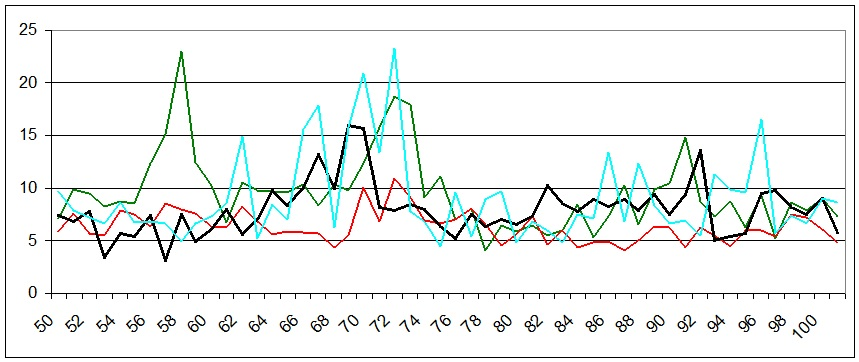
\includegraphics[width=0.8\textwidth]{sperimentazioni/ecotexas/Grafici/Ahead1/Temperatura.jpg}
\caption{Temperatura ahead 1}
\label{TA1}
}
\end{figure}

\medskip

Ahead = 2 

\begin{figure}[H]
\textbf{
\centering
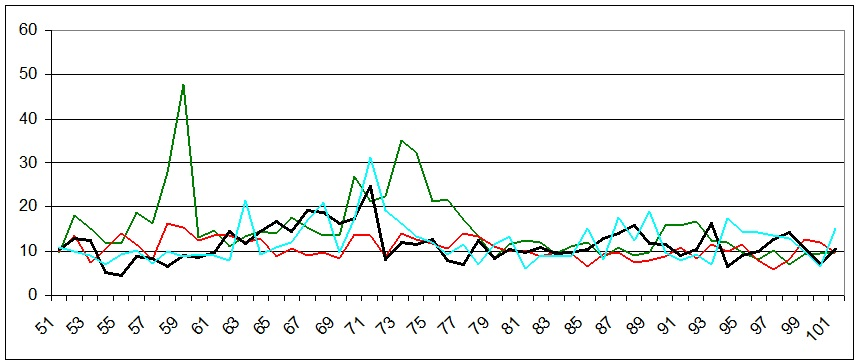
\includegraphics[width=0.8\textwidth]{sperimentazioni/ecotexas/Grafici/Ahead2/Temperatura.jpg}
\caption{Temperatura ahead 2}
\label{TA2}
}
\end{figure}

\newpage

Ahead = 3

\begin{figure}[H]
\textbf{
\centering
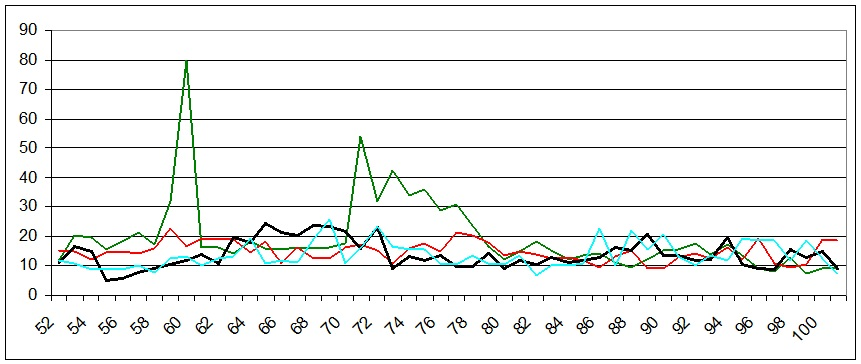
\includegraphics[width=0.8\textwidth]{sperimentazioni/ecotexas/Grafici/Ahead3/Temperatura.jpg}
\caption{Temperatura ahead 3}
\label{TA3}
}
\end{figure}

Ahead = 4 

\begin{figure}[H]
\textbf{
\centering
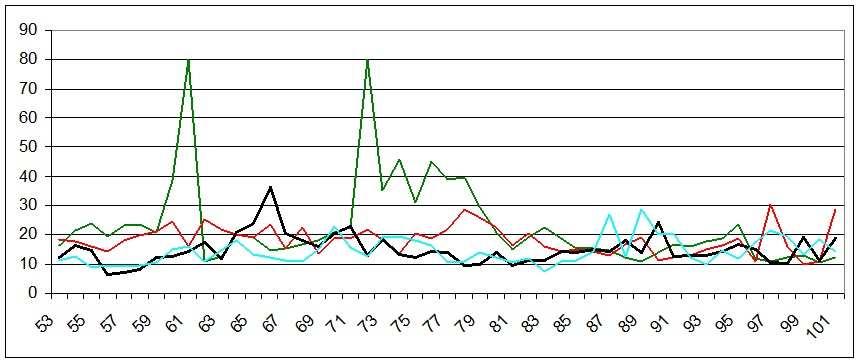
\includegraphics[width=0.8\textwidth]{sperimentazioni/ecotexas/Grafici/Ahead4/Temperatura.jpg}
\caption{Temperatura ahead 4}
\label{TA4}
}
\end{figure}

Ahead = 5

\begin{figure}[H]
\textbf{
\centering
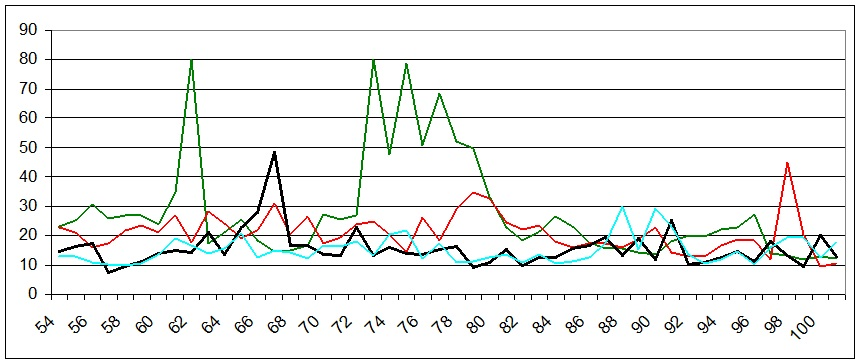
\includegraphics[width=0.8\textwidth]{sperimentazioni/ecotexas/Grafici/Ahead5/Temperatura.jpg}
\caption{Temperatura ahead 5}
\label{TA5}
}
\end{figure}

Ahead = 6 

\begin{figure}[H]
\textbf{
\centering
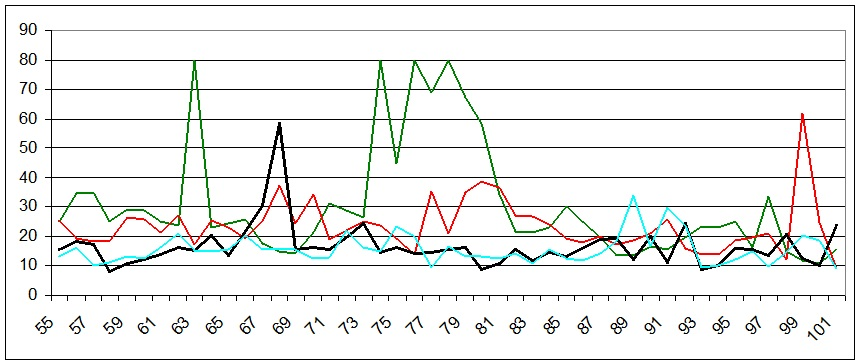
\includegraphics[width=0.8\textwidth]{sperimentazioni/ecotexas/Grafici/Ahead6/Temperatura.jpg}
\caption{Temperatura ahead 6}
\label{TA6}
}
\end{figure}

\textbf{Attributo: Velocità del vento}

\medskip

Ahead = 1

\begin{figure}[H]
\textbf{
\centering
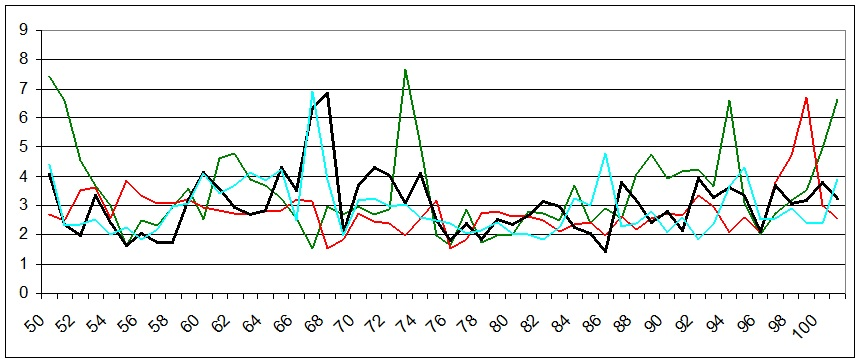
\includegraphics[width=0.8\textwidth]{sperimentazioni/ecotexas/Grafici/Ahead1/Vento.jpg}
\caption{Velocità vento ahead 1}
\label{VA1}
}
\end{figure}

Ahead = 2 

\begin{figure}[H]
\textbf{
\centering
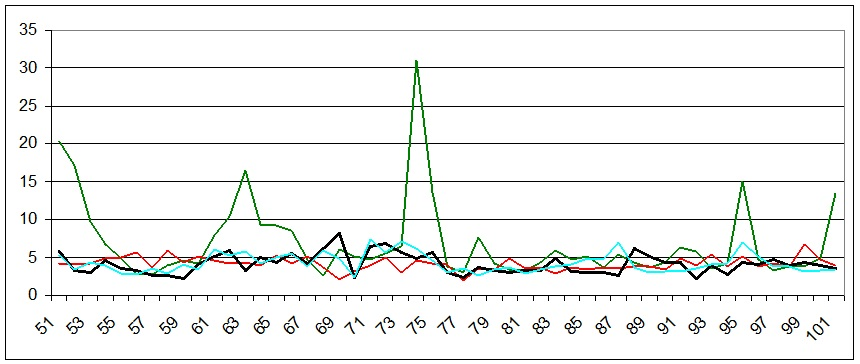
\includegraphics[width=0.8\textwidth]{sperimentazioni/ecotexas/Grafici/Ahead2/Vento.jpg}
\caption{Velocità vento ahead 2}
\label{VA2}
}
\end{figure}

Ahead = 3

\begin{figure}[H]
\textbf{
\centering
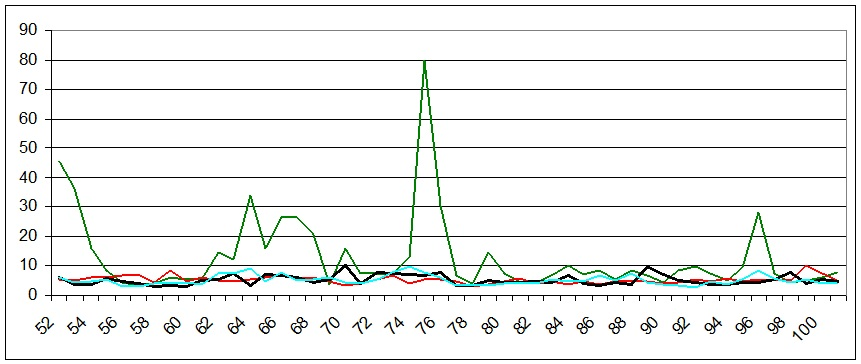
\includegraphics[width=0.8\textwidth]{sperimentazioni/ecotexas/Grafici/Ahead3/Vento.jpg}
\caption{Velocità vento ahead 3}
\label{VA3}
}
\end{figure}

Ahead = 4 

\begin{figure}[H]
\textbf{
\centering
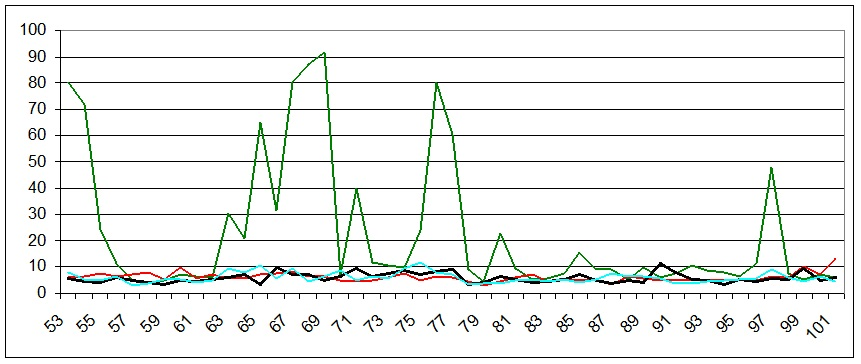
\includegraphics[width=0.8\textwidth]{sperimentazioni/ecotexas/Grafici/Ahead4/Vento.jpg}
\caption{Velocità vento ahead 4}
\label{VA4}
}
\end{figure}

Ahead = 5

\begin{figure}[H]
\textbf{
\centering
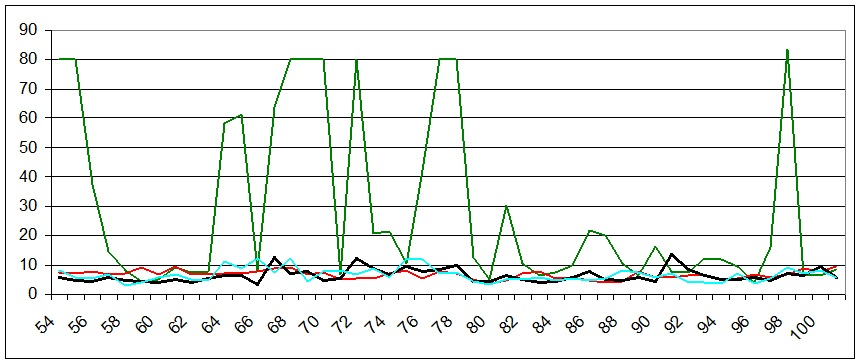
\includegraphics[width=0.8\textwidth]{sperimentazioni/ecotexas/Grafici/Ahead5/Vento.jpg}
\caption{Velocità vento ahead 5}
\label{VA5}
}
\end{figure}

Ahead = 6 

\begin{figure}[H]
\textbf{
\centering
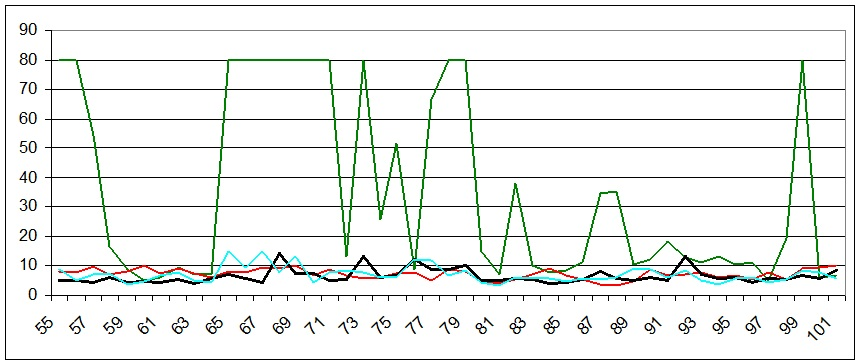
\includegraphics[width=0.8\textwidth]{sperimentazioni/ecotexas/Grafici/Ahead6/Vento.jpg}
\caption{Velocità vento ahead 6}
\label{VA6}
}
\end{figure}

\textbf{Attributo: Ozono}

Ahead = 1

\begin{figure}[H]
\textbf{
\centering
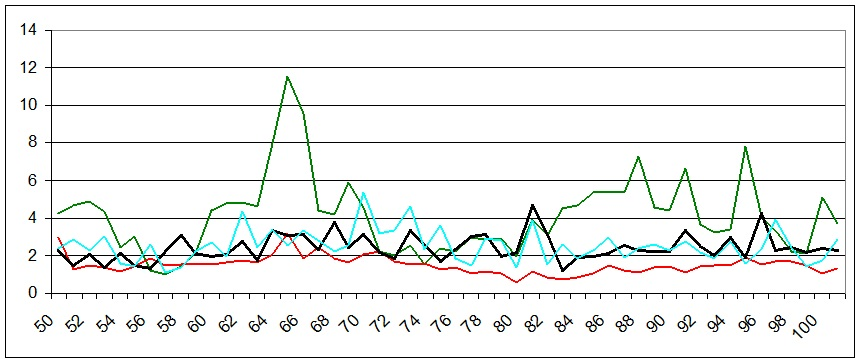
\includegraphics[width=0.8\textwidth]{sperimentazioni/ecotexas/Grafici/Ahead1/Ozono.jpg}
\caption{Ozono ahead 1}
\label{OA1}
}
\end{figure}

Ahead = 2 

\begin{figure}[H]
\textbf{
\centering
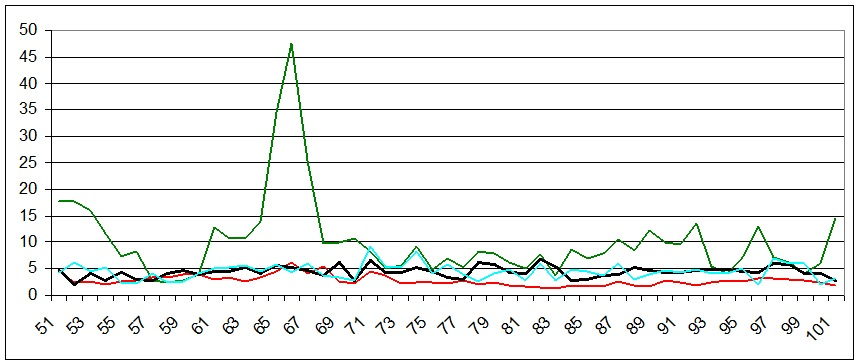
\includegraphics[width=0.8\textwidth]{sperimentazioni/ecotexas/Grafici/Ahead2/Ozono.jpg}
\caption{Ozono ahead 2}
\label{OA2}
}
\end{figure}

Ahead = 3

\begin{figure}[H]
\textbf{
\centering
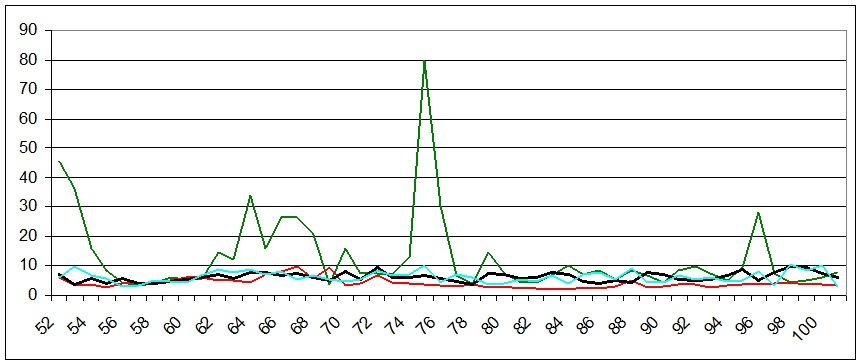
\includegraphics[width=0.8\textwidth]{sperimentazioni/ecotexas/Grafici/Ahead3/Ozono.jpg}
\caption{Ozono ahead 3}
\label{OA3}
}
\end{figure}

Ahead = 4 

\begin{figure}[H]
\textbf{
\centering
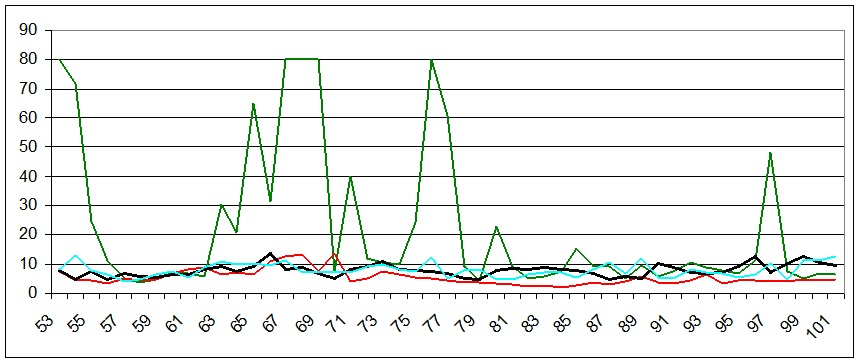
\includegraphics[width=0.8\textwidth]{sperimentazioni/ecotexas/Grafici/Ahead4/Ozono.jpg}
\caption{Ozono ahead 4}
\label{OA4}
}
\end{figure}

Ahead = 5

\begin{figure}[H]
\textbf{
\centering
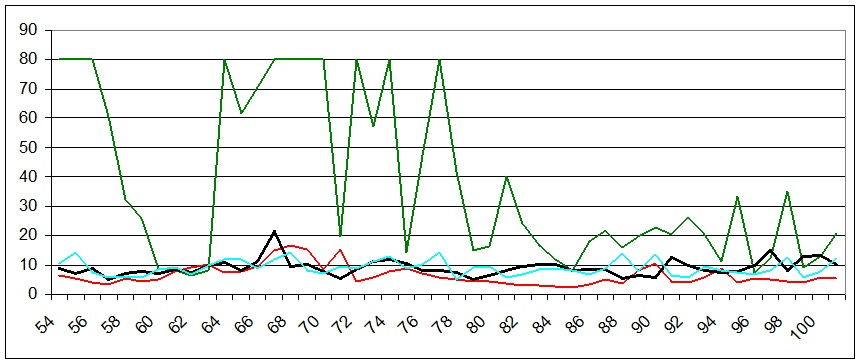
\includegraphics[width=0.8\textwidth]{sperimentazioni/ecotexas/Grafici/Ahead5/Ozono.jpg}
\caption{Ozono ahead 5}
\label{OA5}
}
\end{figure}

Ahead = 6 

\begin{figure}[H]
\textbf{
\centering
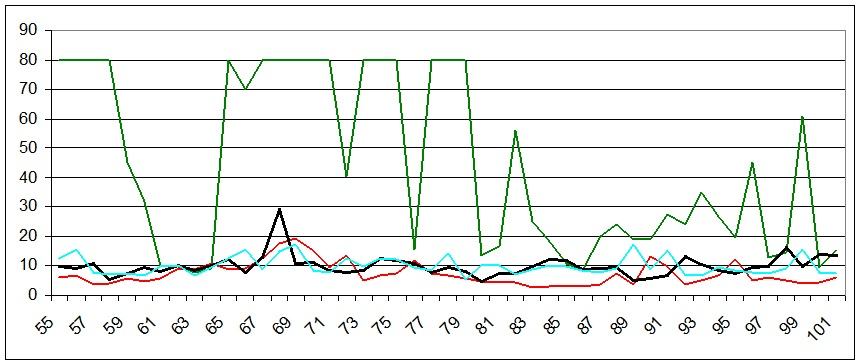
\includegraphics[width=0.8\textwidth]{sperimentazioni/ecotexas/Grafici/Ahead6/Ozono.jpg}
\caption{Ozono ahead 6}
\label{OA6}
}
\end{figure}

\textbf{Attributo: Radiazioni solari}

Ahead = 1

\begin{figure}[H]
\textbf{
\centering
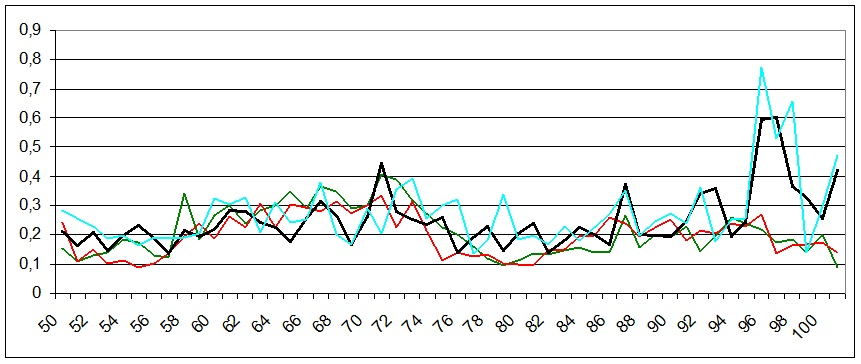
\includegraphics[width=0.8\textwidth]{sperimentazioni/ecotexas/Grafici/Ahead1/Radiazioni.jpg}
\caption{Radiazioni ahead 1}
\label{RA1}
}
\end{figure}

Ahead = 2 

\begin{figure}[H]
\textbf{
\centering
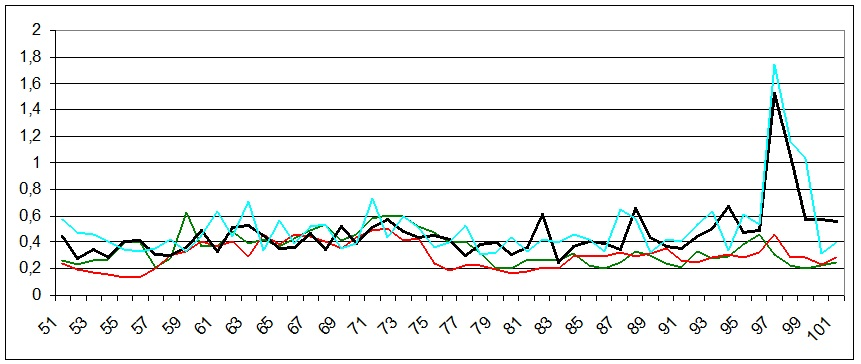
\includegraphics[width=0.8\textwidth]{sperimentazioni/ecotexas/Grafici/Ahead2/Radiazioni.jpg}
\caption{Radiazioni ahead 2}
\label{RA2}
}
\end{figure}

Ahead = 3

\begin{figure}[H]
\textbf{
\centering
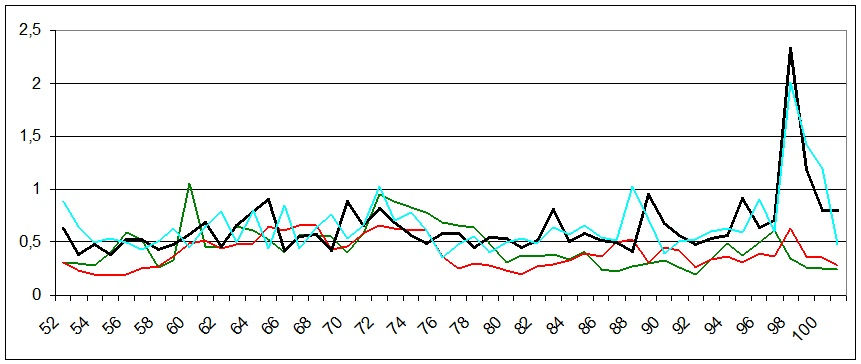
\includegraphics[width=0.8\textwidth]{sperimentazioni/ecotexas/Grafici/Ahead3/Radiazioni.jpg}
\caption{Radiazioni ahead 3}
\label{RA3}
}
\end{figure}

Ahead = 4 

\begin{figure}[H]
\textbf{
\centering
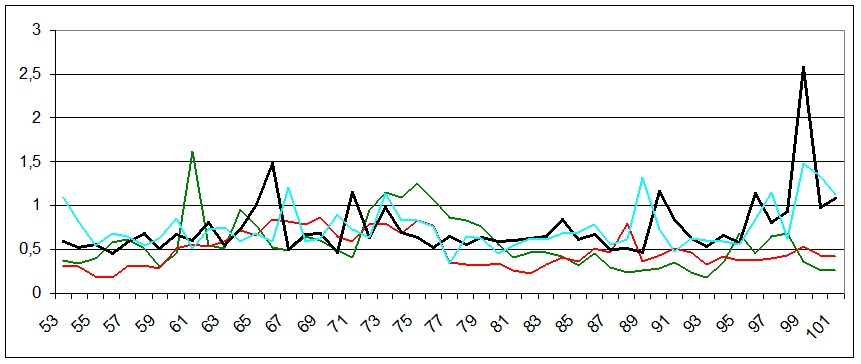
\includegraphics[width=0.8\textwidth]{sperimentazioni/ecotexas/Grafici/Ahead4/Radiazioni.jpg}
\caption{Radiazioni ahead 4}
\label{RA4}
}
\end{figure}

Ahead = 5

\begin{figure}[H]
\textbf{
\centering
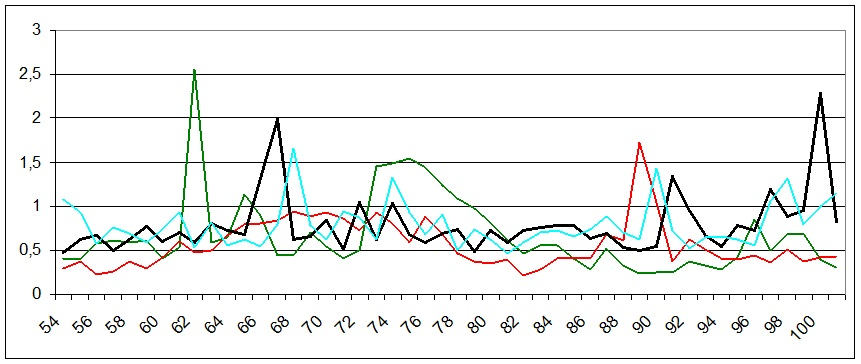
\includegraphics[width=0.8\textwidth]{sperimentazioni/ecotexas/Grafici/Ahead5/Radiazioni.jpg}
\caption{Radiazioni ahead 5}
\label{RA5}
}
\end{figure}

Ahead = 6 

\begin{figure}[H]
\textbf{
\centering
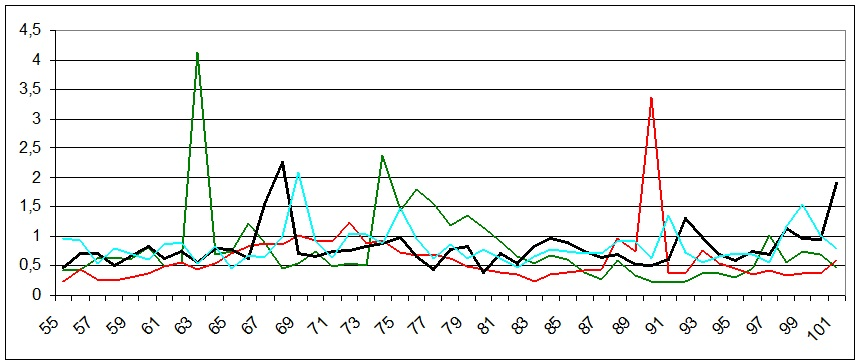
\includegraphics[width=0.8\textwidth]{sperimentazioni/ecotexas/Grafici/Ahead6/Radiazioni.jpg}
\caption{Radiazioni ahead 6}
\label{RA6}
}
\end{figure}

Come è possibile vedere da Fig.~\ref{TA1} a Fig.~\ref{RA6}, gli RMSE generati dalle previsioni effettuate con le versioni VARForecaster 2.1 e VARForecaster 2.2 non si discostano molto da quelli generati dalla versione VARForecaster 1.0, soprattutto con l'aumentare della distanze nel tempo (ahead) con cui si effettua la previsione.

Questo mostra che le due versioni sopracitate realizzano l'obiettivo di costruire previsioni sufficientemente accurate, eseguendo la computazione in tempi ragionevoli.
\newpage
\subsection{UnitedStatesPacific}
Per il dataset UnitedStatesPacific sono stati utilizzati i seguenti parametri:

\begin{center}
\begin{table}[H]
\centering
\begin{tabular}{|c|c|}
\hline
\textbf{Dimensione finestra temporale} & 48 \\
\hline
\textbf{bperc.} & 0.1f \\
\hline
\textbf{lag.max} & 24 \\
\hline
\textbf{Season} & NULL \\
\hline
\textbf{Exogen} & NULL \\
\hline
\textbf{ic} & ALL \\
\hline
\textbf{type} & ALL \\
\hline
\textbf{n.ahead} & 6 \\
\hline
\end{tabular}
\caption{Parametri per UnitedStatesPacific}
\end{table}
\end{center}
dove "ALL" indica che è il sistema a trovare il parametro ottimale tra quelli ammissibili per la costruzione del modello VAR.

\medskip

\subsubsection{VARForecaster 2.1}

Come per il dataset Ecotexas, per la versione VARForecaster 2.1 ci sono quattro possibili configurazioni, ovvero:
\begin{enumerate}
\item Calcolo dell'aggregato con utilizzo della media e indice di autocorrelazione spaziale Getis and Ord;
\item Calcolo dell'aggregato con utilizzo della mediana e indice di autocorrelazione spaziale Getis and Ord;
\item Calcolo dell'aggregato con utilizzo della media e varianza;
\item Calcolo dell'aggregato con utilizzo della mediana e varianza;
\end{enumerate}
Sono di seguito riportati i risultati avuti attraverso le valutazioni delle metriche \textit{(1)} e \textit{(2)} (definite in Sezione 4.1).

\newpage

\textbf{Metrica 1: Media dello RMSE per ogni istante di tempo predetto} \medskip

Attributo: dewp \\ 
\begin{table}[H]
\centering
\begin{tabular}{|c|c|c|c|c|}
\hline
 & \textbf{Media+GO} & \textbf{Mediana+GO} & \textbf{Media+Var} & \textbf{Mediana+Var} \\
\hline
\textbf{ahead 1} & 10,35410 & 8,09983 & 8,49547 & \textbf{4,57026} \\
\hline
\textbf{ahead 2} & 21,61805 & 11,76371 & 13,28951 & \textbf{8,98220} \\
\hline
\textbf{ahead 3} & 45,65774 & 17,53932 & 15,10214 & \textbf{10,6661} \\
\hline
\textbf{ahead 4} & 102,77642 & 23,89249 & 22,33428 & \textbf{13,1286} \\
\hline
\textbf{ahead 5} & 253,97965 & 46,02549 & 33,96732 & \textbf{15,46501} \\
\hline
\textbf{ahead 6} & 696,45082 & 73,04417 & 43,15385 & \textbf{17,87788} \\
\hline
\end{tabular} \\
\caption{UnitedStatesPacific VARForecaster 2.1 - Metrica \textit{(1)}, dewp}
\end{table} 

\medskip

Attributo: pres \\ 

\begin{table}[H]
\centering
\begin{tabular}{|c|c|c|c|c|}
\hline
 & \textbf{Media+GO} & \textbf{Mediana+GO} & \textbf{Media+Var} & \textbf{Mediana+Var} \\
\hline
\textbf{ahead 1} & 21,28281 & 20,75721 & 4,29425 & \textbf{3,50544} \\
\hline
\textbf{ahead 2} & 27,66193 & 26,17847 & 8,09658 & \textbf{6,21739} \\
\hline
\textbf{ahead 3} & 37,6824 & 33,0506 & 11,1886 & \textbf{7,80243} \\
\hline
\textbf{ahead 4} & 48,2233 & 28,368 & 17,60297 & \textbf{9,42102} \\
\hline
\textbf{ahead 5} & 111,7456 & 39,39191 & 22,80009 & \textbf{11,24487} \\
\hline
\textbf{ahead 6} & 282,6471 & 54,53949 & 33,8591 & \textbf{11,85886} \\
\hline
\end{tabular} \\
\caption{UnitedStatesPacific VARForecaster 2.1 - Metrica \textit{(1)}, pres}
\end{table}

\medskip

Attributo:temp \\ 

\begin{table}[H]
\centering
\begin{tabular}{|c|c|c|c|c|}
\hline
 & \textbf{Media+GO} & \textbf{Mediana+GO} & \textbf{Media+Var} & \textbf{Mediana+Var} \\
\hline
\textbf{ahead 1} & 15,44130 & 12,99331 & 17,00225 & \textbf{10,82273} \\
\hline
\textbf{ahead 2} & 33,28733 & 23,22106 & 33,9441 & \textbf{18,33721} \\
\hline
\textbf{ahead 3} & 69,6794 & 38,8886 & 39,2455 & \textbf{22,9628} \\
\hline
\textbf{ahead 4} & 157,924 & 57,0033 & 64,748 & \textbf{28,9879} \\
\hline
\textbf{ahead 5} & 384,654 & 113,0101 & 105,5124 & \textbf{35,12572} \\
\hline
\textbf{ahead 6} & 989,1974 & 186,4416 & 173,5766 & \textbf{41,29017} \\
\hline
\end{tabular} \\
\caption{UnitedStatesPacific VARForecaster 2.1 - Metrica \textit{(1)}, temp}
\end{table}

\medskip

Attributo: wind \\ 

\begin{table}[H]
\centering
\begin{tabular}{|c|c|c|c|c|}
\hline
 & \textbf{Media+GO} & \textbf{Mediana+GO} & \textbf{Media+Var} & \textbf{Mediana+Var} \\
\hline
\textbf{ahead 1} & 9,65734 & 7,80671 & 5,31065 & \textbf{4,38076} \\
\hline
\textbf{ahead 2} & 16,47911 & 11,33491 & 11,50816 & \textbf{7,804106} \\
\hline
\textbf{ahead 3} & 27,5363 & 12,3545 & 13,4658 & \textbf{8,44543} \\
\hline
\textbf{ahead 4} & 64,596 & 11,7299 & 17,3327 & \textbf{9,52957} \\
\hline
\textbf{ahead 5} & 156,9214 & \textbf{5,29247} & 27,69262 & 11,75549 \\
\hline
\textbf{ahead 6} & 403,6115 & 25,75966 & 44,38998 & \textbf{12,72086} \\
\hline
\end{tabular}
\caption{UnitedStatesPacific VARForecaster 2.1 - Metrica \textit{(1)}, wind}
\end{table}
\newpage

\textbf{Metrica 2: Deviazione standard dello RMSE per ogni istante di tempo predetto}

\medskip


Attributo: dewp \\

\begin{table}[H]
\centering
\begin{tabular}{|c|c|c|c|c|}
\hline
 & \textbf{Media+GO} & \textbf{Mediana+GO} & \textbf{Media+Var} & \textbf{Mediana+Var} \\
\hline
\textbf{ahead 1} & 5,94495 & 2,16626 & 2,58476 & \textbf{1,56471} \\
\hline
\textbf{ahead 2} & 18,00577 & 4,07715 & 5,34757 & \textbf{2,65384} \\
\hline
\textbf{ahead 3} & 54,40966 & 14,23701 & 7,42695 & \textbf{3,41018} \\
\hline
\textbf{ahead 4} & 149,69459 & 26,32336 & 14,57913 & \textbf{4,49271} \\
\hline
\textbf{ahead 5} & 434,63121 & 127,65742 & 35,53876 & \textbf{6,16542} \\
\hline
\textbf{ahead 6} & 1520,89339 & 256,50925 & 60,91395 & \textbf{9,84278} \\
\hline
\end{tabular} \\
\caption{UnitedStatesPacific VARForecaster 2.1 - Metrica \textit{(2)}, dewp}
\end{table}

\medskip

Attributo: pres \\ 

\begin{table}[H]
\centering
\begin{tabular}{|c|c|c|c|c|}
\hline
 & \textbf{Media+GO} & \textbf{Mediana+GO} & \textbf{Media+Var} & \textbf{Mediana+Var} \\
\hline
\textbf{ahead 1} & 16,43563 & 16,62778 & 1,54870 & \textbf{1,17519} \\
\hline
\textbf{ahead 2} & 18,85916 & 19,19468 & 2,73254 & \textbf{1,75573} \\
\hline
\textbf{ahead 3} & 20,2104 & 19,5822 & 4,24635 & \textbf{2,72991} \\
\hline
\textbf{ahead 4} & 45,4935 & 18,2257 & 9,91846 & \textbf{3,5497} \\
\hline
\textbf{ahead 5} & 163,0839 & 56,70568 & 11,96975 & \textbf{6,70423} \\
\hline
\textbf{ahead 6} & 567,2065 & 134,0601 & 50,99903 & \textbf{8,51059} \\
\hline
\end{tabular} \\
\caption{UnitedStatesPacific VARForecaster 2.1 - Metrica \textit{(2)}, pres}
\end{table}

\medskip

Attributo: temp \\ 

\begin{table}[H]
\centering
\begin{tabular}{|c|c|c|c|c|}
\hline
 & \textbf{Media+GO} & \textbf{Mediana+GO} & \textbf{Media+Var} & \textbf{Mediana+Var} \\
\hline
\textbf{ahead 1} & 6,31481 & 3,27786 & 6,12472 & \textbf{4,61221} \\
\hline
\textbf{ahead 2} & 19,84917 & 8,63296 & 14,53473 & \textbf{5,97245} \\
\hline
\textbf{ahead 3} & 68,9712 & 27,2828 & 24,1208 & 8\textbf{,71251} \\
\hline
\textbf{ahead 4} & 194,173 & 56,199 & 66,6488 & \textbf{12,4755} \\
\hline
\textbf{ahead 5} & 520,5953 & 242,3278 & 139,1948 & \textbf{8,23943} \\
\hline
\textbf{ahead 6} & 1644,085 & 525,6508 & 321,1888 & \textbf{29,11351} \\
\hline
\end{tabular} \\
\caption{UnitedStatesPacific VARForecaster 2.1 - Metrica \textit{(2)}, temp}
\end{table}

\medskip

Attributo: wind \\ 

\begin{table}[H]
\centering
\begin{tabular}{|c|c|c|c|c|}
\hline
 & \textbf{Media+GO} & \textbf{Mediana+GO} & \textbf{Media+Var} & \textbf{Mediana+Var} \\
\hline
\textbf{ahead 1} & 5,37025 & 5,18403 & \textbf{2,06998} & 2,16056 \\
\hline
\textbf{ahead 2} & 10,94917 & 6,84611 & 5,02589 & \textbf{3,63488} \\
\hline
\textbf{ahead 3} & 29,7911 & 5,89965 & 7,45265 & \textbf{3,80555} \\
\hline
\textbf{ahead 4} & 106,774 & 4,05948 & 16,011 & \textbf{4,99517} \\
\hline
\textbf{ahead 5} & 304,1241 & 9,96997 & 29,86768 & \textbf{5,47922} \\
\hline
\textbf{ahead 6} & 918,9793 & 16,76353 & 65,30511 & \textbf{7,00446} \\
\hline
\end{tabular} 
\caption{UnitedStatesPacific VARForecaster 2.1 - Metrica \textit{(2)}, wind}
\end{table}
\newpage
Per entrambe le metriche sono riportati in \textbf{grassetto} gli RMSE più bassi ottenuti per ogni istante temporale previsto. 

Per meglio comprendere questi risultati si riportano nel seguito le tabelle, una per ogni istante di tempo di previsione (ahead), riportanti il numero di volte che una configurazione è stata scelta come migliore.

\medskip
\textbf{Ahead = 1}


\begin{table}[H]
\centering
\begin{tabular}{|c|c|c|c|c|c|c|c|c|c|c|c|c|}
\hline
 & \multicolumn{4}{|c|}{\textbf{Totale}} & \multicolumn{4}{|c|}{\textbf{Metrica 1}} & \multicolumn{4}{|c|}{\textbf{Metrica 2}} \\
\hline
\textbf{Configurazioni} & 1 & 2 & 3 & \textbf{4} & 1 & 2 & 3 & 4 & 1 & 2 & 3 & 4 \\
\hline
\textbf{Occorrenze} & 0 & 0 & 1 & \textbf{7} & 0 & 0 & 0 & 4 & 0 & 0 & 1 & 3\\
\hline
\end{tabular}
\caption{UnitedStatesPacific VARForecaster 2.1 - Riassunto Ahead 1}
\end{table}

\medskip
\textbf{Ahead = 2}


\begin{table}[H]
\centering
\begin{tabular}{|c|c|c|c|c|c|c|c|c|c|c|c|c|}
\hline
 & \multicolumn{4}{|c|}{\textbf{Totale}} & \multicolumn{4}{|c|}{\textbf{Metrica 1}} & \multicolumn{4}{|c|}{\textbf{Metrica 2}} \\
\hline
\textbf{Configurazioni} & 1 & 2 & 3 & \textbf{4} & 1 & 2 & 3 & 4 & 1 & 2 & 3 & 4 \\
\hline
\textbf{Occorrenze} & 0 & 0 & 0 & \textbf{8} & 0 & 0 & 0 & 4 & 0 & 0 & 0 & 4\\
\hline
\end{tabular}
\caption{UnitedStatesPacific VARForecaster 2.1 - Riassunto Ahead 2}
\end{table}

\medskip
\textbf{Ahead = 3}


\begin{table}[H]
\centering
\begin{tabular}{|c|c|c|c|c|c|c|c|c|c|c|c|c|}
\hline
 & \multicolumn{4}{|c|}{\textbf{Totale}} & \multicolumn{4}{|c|}{\textbf{Metrica 1}} & \multicolumn{4}{|c|}{\textbf{Metrica 2}} \\
\hline
\textbf{Configurazioni} & 1 & 2 & 3 & \textbf{4} & 1 & 2 & 3 & 4 & 1 & 2 & 3 & 4 \\
\hline
\textbf{Occorrenze} & 0 & 0 & 0 & \textbf{8} & 0 & 0 & 0 & 4 & 0 & 0 & 0 & 4\\
\hline
\end{tabular}
\caption{UnitedStatesPacific VARForecaster 2.1 - Riassunto Ahead 3}
\end{table}

\medskip
\textbf{Ahead = 4}


\begin{table}[H]
\centering
\begin{tabular}{|c|c|c|c|c|c|c|c|c|c|c|c|c|}
\hline
 & \multicolumn{4}{|c|}{\textbf{Totale}} & \multicolumn{4}{|c|}{\textbf{Metrica 1}} & \multicolumn{4}{|c|}{\textbf{Metrica 2}} \\
\hline
\textbf{Configurazioni} & 1 & 2 & 3 & \textbf{4} & 1 & 2 & 3 & 4 & 1 & 2 & 3 & 4 \\
\hline
\textbf{Occorrenze} & 0 & 0 & 0 & \textbf{8} & 0 & 0 & 0 & 4 & 0 & 0 & 0 & 4\\
\hline
\end{tabular}
\caption{UnitedStatesPacific VARForecaster 2.1 - Riassunto Ahead 4}
\end{table}

\medskip
\textbf{Ahead = 5}


\begin{table}[H]
\centering
\begin{tabular}{|c|c|c|c|c|c|c|c|c|c|c|c|c|}
\hline
 & \multicolumn{4}{|c|}{\textbf{Totale}} & \multicolumn{4}{|c|}{\textbf{Metrica 1}} & \multicolumn{4}{|c|}{\textbf{Metrica 2}} \\
\hline
\textbf{Configurazioni} & 1 & 2 & 3 & \textbf{4} & 1 & 2 & 3 & 4 & 1 & 2 & 3 & 4 \\
\hline
\textbf{Occorrenze} & 0 & 1 & 0 & \textbf{7} & 0 & 1 & 0 & 3 & 0 & 0 & 0 & 4\\
\hline
\end{tabular}
\caption{UnitedStatesPacific VARForecaster 2.1 - Riassunto Ahead 5}
\end{table}

\medskip
\textbf{Ahead = 6}


\begin{table}[H]
\centering
\begin{tabular}{|c|c|c|c|c|c|c|c|c|c|c|c|c|}
\hline
 & \multicolumn{4}{|c|}{\textbf{Totale}} & \multicolumn{4}{|c|}{\textbf{Metrica 1}} & \multicolumn{4}{|c|}{\textbf{Metrica 2}} \\
\hline
\textbf{Configurazioni} & 1 & 2 & 3 & \textbf{4} & 1 & 2 & 3 & 4 & 1 & 2 & 3 & 4 \\
\hline
\textbf{Occorrenze} & 0 & 0 & 0 & \textbf{8} & 0 & 0 & 0 & 4 & 0 & 0 & 0 & 4\\
\hline
\end{tabular}
\caption{UnitedStatesPacific VARForecaster 2.1 - Riassunto Ahead 6}
\end{table} 

\medskip

In base alle metriche \textit{(1)} e \textit{(2)}, utilizzate per valutare l'accuratezza del sistema, è possibile notare come la configurazione migliore (più accurata) è indubbiamente la 4, nonché \textbf{mediana + varianza}.

\medskip

\textbf{Metrica 4: Tempo medio di computazione per la costruzione(/riapprendimento) del \textit{CT}.}

\medskip


\begin{table}[H]
\centering
\begin{tabular}[H]{|c|c|c|c|}
\hline
\textbf{Media+GO} & \textbf{Mediana+GO} & \textbf{Media+Var} & \textbf{Mediana+Var} \\
\hline
\textbf{4,44} & 5,35 & 29,71 & 36,10 \\
\hline
\end{tabular}
\caption{UnitedStatesPacific VARForecaster 2.1 - Metrica \textit{(4)}}
\end{table} 

\medskip 
\textbf{Metrica 5: Tempo medio di computazione per l'apprendimento del modello VAR.}

\medskip

\begin{table}[H]
\centering
\begin{tabular}[H]{|c|c|c|c|}
\hline
\textbf{Media+GO} & \textbf{Mediana+GO} & \textbf{Media+Var} & \textbf{Mediana+Var} \\
\hline
18526 & 19324 & \textbf{16009} & 16237\\
\hline
\end{tabular}
\caption{UnitedStatesPacific VARForecaster 2.1 - Metrica \textit{(5)}}
\end{table} 

\medskip 
\textbf{Metrica 6: Tempo medio di computazione per la fase di previsione.}

\medskip


\begin{table}[H]
\centering
\begin{tabular}[H]{|c|c|c|c|}
\hline
\textbf{Media+GO} & \textbf{Mediana+GO} & \textbf{Media+Var} & \textbf{Mediana+Var} \\
\hline
\textbf{3,49} & 4,28 & 3,87 & 4,02 \\
\hline
\end{tabular}
\caption{UnitedStatesPacific VARForecaster 2.1 - Metrica \textit{(6)}}
\end{table} 

\newpage

\subsubsection{VARForecaster 2.2}

Sono di seguito nuovamente elencate le configurazioni possibili per la versione VARForecaster 2.2:
\begin{enumerate}
\item Apprendimento dell'albero con algoritmo di smoothing utilizzando un $ \alpha = 0.4$, calcolo dell'aggregato con la mediana e indice di autocorrelazione spaziale Getis and Ord.
\item Apprendimento dell'albero con algoritmo di smoothing utilizzando un $ \alpha = 0.4$, calcolo dell'aggregato con la media e indice di autocorrelazione spaziale Getis and Ord.
\item Apprendimento dell'albero con algoritmo di smoothing utilizzando un $ \alpha = 0.4$, calcolo dell'aggregato con la mediana e varianza.
\item Apprendimento dell'albero con algoritmo di smoothing utilizzando un $ \alpha = 0.4$, calcolo dell'aggregato con la media e varianza.
\item Apprendimento dell'albero con algoritmo di smoothing utilizzando un $ \alpha = 0.5$, calcolo dell'aggregato con la mediana e indice di autocorrelazione spaziale Getis and Ord.
\item Apprendimento dell'albero con algoritmo di smoothing utilizzando un $ \alpha = 0.5$, calcolo dell'aggregato con la media e indice di autocorrelazione spaziale Getis and Ord.
\item Apprendimento dell'albero con algoritmo di smoothing utilizzando un $ \alpha = 0.5$, calcolo dell'aggregato con la mediana e varianza.
\item Apprendimento dell'albero con algoritmo di smoothing utilizzando un $ \alpha = 0.5$, calcolo dell'aggregato con la media e varianza.
\item Apprendimento dell'albero con algoritmo di smoothing utilizzando un $ \alpha = 0.6$, calcolo dell'aggregato con la mediana e indice di autocorrelazione spaziale Getis and Ord.
\item Apprendimento dell'albero con algoritmo di smoothing utilizzando un $ \alpha = 0.6$, calcolo dell'aggregato con la media e indice di autocorrelazione spaziale Getis and Ord.
\item Apprendimento dell'albero con algoritmo di smoothing utilizzando un $ \alpha = 0.6$, calcolo dell'aggregato con la mediana e varianza.
\item Apprendimento dell'albero con algoritmo di smoothing utilizzando un $ \alpha = 0.6$, calcolo dell'aggregato con la media e varianza.
\end{enumerate}

Per le metriche \textit{(1)} e \textit{(2)} i risultati sono stati analizzati attributo per attributo. Le tabelle sono organizzate in base ai livelli $\alpha$ Ogni tabella, inoltre, include le seguenti quattro colonne:

\begin{enumerate}
\item Calcolo dell'aggregato con utilizzo della media e indice di autocorrelazione spaziale Getis and Ord;
\item Calcolo dell'aggregato con utilizzo della mediana e indice di autocorrelazione spaziale Getis and Ord;
\item Calcolo dell'aggregato con utilizzo della media e varianza;
\item Calcolo dell'aggregato con utilizzo della mediana e varianza;
\end{enumerate}

Sono di seguito riportati i risultati.

\medskip

\textbf{Metrica 1: Media dello RMSE per ogni istante di tempo predetto} \medskip

Attributo: dewp \\ 

\begin{table}[H]
\centering
\begin{tabular}{|c|c|c|c|c|}
\hline
 & \multicolumn{4}{|c|}{Smoothing $\alpha$ = 0.4} \\
\hline
& 1 & 2 & 3 & 4 \\
\hline
\textbf{ahead 1} & 8,27904 & 6,38061 & 8,26531 & 5,27701 \\
\hline
\textbf{ahead 2} & 16,0298 & 10,5766 & 13,6887 & 9,31357\\ 
\hline
\textbf{ahead 3} & 27,42677 & 14,69364 & 17,81315 & 12,46099\\
\hline
\textbf{ahead 4} & 51,20479 & 16,5757 & 28,71257 & 15,34014\\ 
\hline
\textbf{ahead 5} & 176,2468 & 19,39388 & 52,98369 & 18,94659\\
\hline
\textbf{ahead 6} & 820,51833 & 22,73526 & 112,34935 & 21,90584\\ 
\hline
\end{tabular} \\
\caption{UnitedStatesPacific VARForecaster 2.2 - Metrica \textit{(1)}, dewp, $\alpha$ = 0.4}
\end{table} 

\newpage

\begin{table}[H]
\centering
\begin{tabular}{|c|c|c|c|c|}
\hline
 & \multicolumn{4}{|c|}{Smoothing $\alpha$ = 0.5} \\
\hline
& 1 & 2 & 3 & 4 \\
\hline
\textbf{ahead 1} & 10,66219 & 8,07925 & 7,98354 & \textbf{5,09278} \\
\hline
\textbf{ahead 2} & 17,4688 & 12,1913 & 12,8452 & \textbf{9,21612}\\ 
\hline
\textbf{ahead 3} & 27,98501 & 17,7251 & 14,86977 & \textbf{11,62603}\\
\hline
\textbf{ahead 4} & 41,56125 & 20,13368 & 20,62609 & 14,61927\\ 
\hline
\textbf{ahead 5} & 83,43031 & 22,61424 & 31,10648 & 18,14871\\
\hline
\textbf{ahead 6} & 197,90215 & 24,96765 & 49,72840 & 21,25953\\ 
\hline
\end{tabular} \\
\caption{UnitedStatesPacific VARForecaster 2.2 - Metrica \textit{(1)}, dewp, $\alpha$ = 0.5}
\end{table} 

\medskip

\begin{table}[H]
\centering
\begin{tabular}{|c|c|c|c|c|}
\hline
 & \multicolumn{4}{|c|}{Smoothing $\alpha$ = 0.6} \\
\hline
& 1 & 2 & 3 & 4 \\
\hline
\textbf{ahead 1} & 12,07665 & 12,05122 & 8,06145 & 5,15736 \\
\hline
\textbf{ahead 2} & 22,1225 & 20,1751 & 13,1302 & 9,46835 \\ 
\hline
\textbf{ahead 3} & 36,67084 & 26,06997 & 14,58737 & 11,68703\\
\hline
\textbf{ahead 4} & 67,92605 & 43,30007 & 20,00141 & \textbf{14,61657}\\ 
\hline
\textbf{ahead 5} & 171,3545 & 78,08391 & 31,71357 & \textbf{18,08502}\\
\hline
\textbf{ahead 6} & 570,41382 & 238,20854 & 55,43952 & \textbf{21,01571}\\ 
\hline
\end{tabular} \\
\caption{UnitedStatesPacific VARForecaster 2.2 - Metrica \textit{(1)}, dewp, $\alpha$ = 0.6}
\end{table} 

\medskip

Attributo: pres \\ 

\begin{table}[H]
\centering
\begin{tabular}{|c|c|c|c|c|}
\hline
 & \multicolumn{4}{|c|}{Smoothing $\alpha$ = 0.4} \\
\hline
& 1 & 2 & 3 & 4 \\
\hline
\textbf{ahead 1} & 16,92658 & 16,58831 & 4,27934 & 3,60989 \\
\hline
\textbf{ahead 2} & 24,1618 & 23,4025 & 8,4444 & 6,63054\\ 
\hline
\textbf{ahead 3} & 21,03628 & 18,30415 & 12,22256 & 8,302075\\
\hline
\textbf{ahead 4} & 27,64643 & 17,25246 & 18,27703 & 10,29753\\ 
\hline
\textbf{ahead 5} & 61,18393 & 18,62148 & 23,13371 & 11,7856\\
\hline
\textbf{ahead 6} & 203,96921 & 17,09940 & 29,04078 & 11,88881\\ 
\hline
\end{tabular} \\
\caption{UnitedStatesPacific VARForecaster 2.2 - Metrica \textit{(1)}, pres, $\alpha$ = 0.4}
\end{table} 

\medskip

\begin{table}[H]
\centering
\begin{tabular}{|c|c|c|c|c|}
\hline
 & \multicolumn{4}{|c|}{Smoothing $\alpha$ = 0.5} \\
\hline
& 1 & 2 & 3 & 4 \\
\hline
\textbf{ahead 1} & 21,2399 & 20,78155 & 4,26267 & \textbf{3,45036}\\
\hline
\textbf{ahead 2} & 28,0996 & 27,3249 & 8,29079 & \textbf{6,077}\\ 
\hline
\textbf{ahead 3} & 25,33999 & 23,02857 & 11,54404 & 7,48301\\
\hline
\textbf{ahead 4} & 27,67892 & 19,17569 & 17,2736 & \textbf{9,43111}\\ 
\hline
\textbf{ahead 5} & 36,72377 & 16,10743 & 22,88078 & 11,27574\\
\hline
\textbf{ahead 6} & 72,55095 & 17,947 & 29,4564 & 11,54297\\ 
\hline
\end{tabular} \\
\caption{UnitedStatesPacific VARForecaster 2.2 - Metrica \textit{(1)}, pres, $\alpha$ = 0.5}
\end{table} 

\medskip

\begin{table}[H]
\centering
\begin{tabular}{|c|c|c|c|c|}
\hline
 & \multicolumn{4}{|c|}{Smoothing $\alpha$ = 0.6} \\
\hline
& 1 & 2 & 3 & 4 \\
\hline
\textbf{ahead 1} & 29,63628 & 29,71818 & 4,36475 & 3,59517 \\
\hline
\textbf{ahead 2} & 26,4177 & 26,3579 & 8,34811 & 6,24176 \\ 
\hline
\textbf{ahead 3} & 24,72792 & 23,29762 & 11,37082 & \textbf{4,603795} \\
\hline
\textbf{ahead 4} & 43,03939 & 32,4199 & 17,44765 & 9,65899\\ 
\hline
\textbf{ahead 5} & 101,0519 & 46,56281 & 22,39137 & \textbf{11,15838}\\
\hline
\textbf{ahead 6} & 362,18329 & 102,81672 & 25,82343 & \textbf{11,10552}\\ 
\hline
\end{tabular} \\
\caption{UnitedStatesPacific VARForecaster 2.2 - Metrica \textit{(1)}, pres, $\alpha$ = 0.6}
\end{table} 

\medskip

Attributo:temp \\ 

\begin{table}[H]
\centering
\begin{tabular}{|c|c|c|c|c|}
\hline
 & \multicolumn{4}{|c|}{Smoothing $\alpha$ = 0.4} \\
\hline
& 1 & 2 & 3 & 4 \\
\hline
\textbf{ahead 1} & 12,36206 & 11,42628 & 18,74542 & 11,51074 \\
\hline
\textbf{ahead 2} & 9,36371 & \textbf{5,94138} & 24,3968 & 7,70272\\ 
\hline
\textbf{ahead 3} & 44,69455 & 32,11892 & 46,44071 & 25,02006\\
\hline
\textbf{ahead 4} & 85,80132 & 44,62097 & 67,06124 & 32,47087\\ 
\hline
\textbf{ahead 5} & 230,561 & 56,32052 & 103,2566 & 38,73074\\
\hline
\textbf{ahead 6} & 921,5452 & 64,9213 & 183,35248 & 44,25375\\ 
\hline
\end{tabular} \\
\caption{UnitedStatesPacific VARForecaster 2.2 - Metrica \textit{(1)}, temp, $\alpha$ = 0.4}
\end{table} 

\medskip

\begin{table}[H]
\centering
\begin{tabular}{|c|c|c|c|c|}
\hline
 & \multicolumn{4}{|c|}{Smoothing $\alpha$ = 0.5} \\
\hline
& 1 & 2 & 3 & 4 \\
\hline
\textbf{ahead 1} & 16,27052 & 11,53227 & 17,45441 & 11,58477 \\
\hline
\textbf{ahead 2} & 17,5606 & 8,87091 & 21,7589 & 7,34922\\ 
\hline
\textbf{ahead 3} & 64,48934 & 42,85104 & 43,7311 & 24,07154 \\
\hline
\textbf{ahead 4} & 99,7284 & 59,6736 & 58,4439 & 30,78391\\ 
\hline
\textbf{ahead 5} & 170,8852 & 73,55237 & 86,44128 & \textbf{36,62066}\\
\hline
\textbf{ahead 6} & 352,27301 & 81,07127 & 145,83875 & \textbf{42,34479}\\ 
\hline
\end{tabular} \\
\caption{UnitedStatesPacific VARForecaster 2.2 - Metrica \textit{(1)}, temp, $\alpha$ = 0.5}
\end{table} 

\medskip

\begin{table}[H]
\centering
\begin{tabular}{|c|c|c|c|c|}
\hline
 & \multicolumn{4}{|c|}{Smoothing $\alpha$ = 0.6} \\
\hline
& 1 & 2 & 3 & 4 \\
\hline
\textbf{ahead 1} & 16,30139 & 14,9276 & 18,06174 & \textbf{11,31821} \\
\hline
\textbf{ahead 2} & 18,9689 & 11,1877 & 21,4415 & 16,83391\\ 
\hline
\textbf{ahead 3} & 84,01594 & 42,38011 & 42,82521 & \textbf{23,4737}\\
\hline
\textbf{ahead 4} & 239,247 & 70,30667 & 54,54914 & \textbf{30,15269}\\ 
\hline
\textbf{ahead 5} & 951,9507 & 110,8372 & 76,20901 & 36,96072\\
\hline
\textbf{ahead 6} & 4724,37274 & 198,39152 & 126,65686 & 42,52642\\ 
\hline
\end{tabular} \\
\caption{UnitedStatesPacific VARForecaster 2.2 - Metrica \textit{(1)}, temp, $\alpha$ = 0.6}
\end{table} 

\medskip


Attributo: wind \\ 

\begin{table}[H]
\centering
\begin{tabular}{|c|c|c|c|c|}
\hline
 & \multicolumn{4}{|c|}{Smoothing $\alpha$ = 0.4} \\
\hline
& 1 & 2 & 3 & 4 \\
\hline
\textbf{ahead 1} & 6,07391 & 5,70323 & 5,97786 & 5,11227 \\
\hline
\textbf{ahead 2} & 3,0769 & \textbf{2,74313} & 12,244 & 4,93367 \\ 
\hline
\textbf{ahead 3} & 14,0015 & 9,395732 & 17,97835 & 9,146756\\
\hline
\textbf{ahead 4} & 23,06176 & 11,03524 & 24,73806 & 11,13321\\ 
\hline
\textbf{ahead 5} & 55,22912 & 12,99234 & 41,2732 & 12,82012\\
\hline
\textbf{ahead 6} & 116,701 & 14,45873 & 79,08570 & 12,98682 \\
\hline
\end{tabular} \\
\caption{UnitedStatesPacific VARForecaster 2.2 - Metrica \textit{(1)}, wind, $\alpha$ = 0.4}
\end{table} 

\medskip

\begin{table}[H]
\centering
\begin{tabular}{|c|c|c|c|c|}
\hline
 & \multicolumn{4}{|c|}{Smoothing $\alpha$ = 0.5} \\
\hline
& 1 & 2 & 3 & 4 \\
\hline
\textbf{ahead 1} & 7,52321 & 6,63368 & 5,86253 & 4,86708 \\
\hline
\textbf{ahead 2} & 6,28608 & 4,33382 & 10,0958 & 4,78144\\ 
\hline
\textbf{ahead 3} & 17,70545 & 11,24401 & 16,44148 & 8,934127\\
\hline
\textbf{ahead 4} & 27,07973 & 12,60431 & 20,23164 & 10,23597\\ 
\hline
\textbf{ahead 5} & 55,83112 & 14,29877 & 30,1624 & 11,80704\\
\hline
\textbf{ahead 6} & 130,73018 & 17,168838 & 46,21421 & 12,2569\\ 
\hline
\end{tabular} \\
\caption{UnitedStatesPacific VARForecaster 2.2 - Metrica \textit{(1)}, wind, $\alpha$ = 0.5}
\end{table} 

\medskip

\begin{table}[H]
\centering
\begin{tabular}{|c|c|c|c|c|}
\hline
 & \multicolumn{4}{|c|}{Smoothing $\alpha$ = 0.6} \\
\hline
& 1 & 2 & 3 & 4 \\
\hline
\textbf{ahead 1} & 9,59845 & 9,28646 & 5,94993 & \textbf{4,65493} \\
\hline
\textbf{ahead 2} & 5,42531 & 3,18113 & 10,2218 & 4,35038 \\ 
\hline
\textbf{ahead 3} & 23,01827 & 12,45196 & 15,81068 & \textbf{8,422983}\\
\hline
\textbf{ahead 4} & 66,23017 & 19,21566 & 18,68297 & \textbf{9,68644}\\ 
\hline
\textbf{ahead 5} & 272,0654 & 32,82459 & 27,83789 & \textbf{11,75522}\\
\hline
\textbf{ahead 6} & 1384,5733 & 74,11397 & 46,00317 & \textbf{12,20324}\\ 
\hline
\end{tabular} \\
\caption{UnitedStatesPacific VARForecaster 2.2 - Metrica \textit{(1)}, wind, $\alpha$ = 0.6}
\end{table} 
\newpage

\textbf{Metrica 2: Deviazione standard dello RMSE per ogni istante di tempo predetto}

\medskip

Attributo: dewp \\

\begin{table}[H]
\centering
\begin{tabular}{|c|c|c|c|c|}
\hline
 & \multicolumn{4}{|c|}{Smoothing $\alpha$ = 0.4} \\
\hline
& 1 & 2 & 3 & 4 \\
\hline
\textbf{ahead 1} & 3,62146 & 2,21437 & 2,69688 & 1,98897 \\
\hline
\textbf{ahead 2} & 9,90162 & 4,16068 & 4,30406 & 3,36315\\
\hline
\textbf{ahead 3} & 33,2724 & 5,201349 & 9,779709 & 4,742231\\
\hline
\textbf{ahead 4} & 159,51 & \textbf{5,16938} & 27,19474 & 5,57008\\ 
\hline
\textbf{ahead 5} & 895,68387 & \textbf{6,80049} & 79,88217 & 8,580549\\
\hline
\textbf{ahead 6} & 5051,54 & \textbf{10,81451} & 232,51391 & 12,32884\\ 
\hline
\end{tabular} \\
\caption{UnitedStatesPacific VARForecaster 2.2 - Metrica \textit{(2)}, dewp, $\alpha$ = 0.4}
\end{table} 

\medskip

\begin{table}[H]
\centering
\begin{tabular}{|c|c|c|c|c|}
\hline
 & \multicolumn{4}{|c|}{Smoothing $\alpha$ = 0.5} \\
\hline
& 1 & 2 & 3 & 4 \\
\hline
\textbf{ahead 1} & 4,04506 & 3,84309 & 2,89746 & 1,88901\\
\hline
\textbf{ahead 2} & 7,09878 & 4,55632 & 4,90044 & 3,37117\\ 
\hline
\textbf{ahead 3} & 11,84762 & 6,938517 & 6,714971 & 4,476137\\
\hline
\textbf{ahead 4} & 27,19841 & 8,65862 & 14,60174 & 5,44206\\ 
\hline
\textbf{ahead 5} & 92,91261 & 10,01995 & 32,91812 & 8,33261\\
\hline
\textbf{ahead 6} & 3226,15397 & 15,93889 & 98,92583 & 12,58244\\  
\hline
\end{tabular} \\
\caption{UnitedStatesPacific VARForecaster 2.2 - Metrica \textit{(2)}, dewp, $\alpha$ = 0.5}
\end{table} 

\medskip

\begin{table}[H]
\centering
\begin{tabular}{|c|c|c|c|c|}
\hline
 & \multicolumn{4}{|c|}{Smoothing $\alpha$ = 0.6} \\
\hline
& 1 & 2 & 3 & 4 \\
\hline
\textbf{ahead 1} & 4,23088 & 7,28793 & 2,82895 & \textbf{1,75402} \\
\hline
\textbf{ahead 2} & 6,65769 & 10,1984 & 4,66539 & \textbf{3,22088}\\ 
\hline
\textbf{ahead 3} & 21,26428 & 18,23092 & 6,969764 & \textbf{4,255774} \\
\hline
\textbf{ahead 4} & 80,49968 & 62,72078 & 14,82992 & 5,47233\\ 
\hline
\textbf{ahead 5} & 305,9681 & 233,5263 & 38,5938 & 8,288871\\
\hline
\textbf{ahead 6} & 1313,57 & 1021,419 & 120,9813 & 12,47698\\ 
\hline
\end{tabular} \\
\caption{UnitedStatesPacific VARForecaster 2.2 - Metrica \textit{(2)}, dewp, $\alpha$ = 0.6}
\end{table} 

\medskip

Attributo: pres \\ 

\begin{table}[H]
\centering
\begin{tabular}{|c|c|c|c|c|}
\hline
 & \multicolumn{4}{|c|}{Smoothing $\alpha$ = 0.4} \\
\hline
& 1 & 2 & 3 & 4 \\
\hline
\textbf{ahead 1} & 10,10679 & 10,17143 & 1.57424 & 1.34531\\
\hline
\textbf{ahead 2} & 10,876 & 11,1444 & 3,65176 &2,18629 \\ 
\hline
\textbf{ahead 3} & 10,02448 & 8,394604 & 5,422072 & 2,743826 \\
\hline
\textbf{ahead 4} & 34,35737 & 8,07045 & 9,24993 & 3,04091\\ 
\hline
\textbf{ahead 5} & 197,7867 & 11,96599 & 14,89458 & 3,00446\\
\hline
\textbf{ahead 6} & 1120,36108 & 15,53281 & 3146606 & 2,83362\\ 
\hline
\end{tabular} \\
\caption{UnitedStatesPacific VARForecaster 2.2 - Metrica \textit{(2)}, pres, $\alpha$ = 0.4}
\end{table} 

\medskip

\begin{table}[H]
\centering
\begin{tabular}{|c|c|c|c|c|}
\hline
 & \multicolumn{4}{|c|}{Smoothing $\alpha$ = 0.5} \\
\hline
& 1 & 2 & 3 & 4 \\
\hline
\textbf{ahead 1} & 14,29961 & 14,54385 & 1,66226 & \textbf{1,14218} \\
\hline
\textbf{ahead 2} & 13,56029 & 13,66938 & 3,70591 & 2,15068 \\ 
\hline
\textbf{ahead 3} & 13,33688 & 13,3792 & 5,71621 & 2,580855 \\
\hline
\textbf{ahead 4} & 14,87002 & 12,55843 & 9,70296 & \textbf{2,44914}\\ 
\hline
\textbf{ahead 5} & 28,51144 & 8,210878 & 17,13722 & 3,04571\\
\hline
\textbf{ahead 6} & 87,23224 & 12,8405 & 48,78620 & 3,39392\\ 
\hline
\end{tabular} \\
\caption{UnitedStatesPacific VARForecaster 2.2 - Metrica \textit{(2)}, pres, $\alpha$ = 0.5}
\end{table}

\medskip

\begin{table}[H]
\centering
\begin{tabular}{|c|c|c|c|c|}
\hline
 & \multicolumn{4}{|c|}{Smoothing $\alpha$ = 0.6} \\
\hline
& 1 & 2 & 3 & 4 \\
\hline
\textbf{ahead 1} & 14,95718 & 14,84216 & 1,62101 & \textbf{1,19107} \\
\hline
\textbf{ahead 2} & 14,2077 & 14,2458 & 3,49222 & \textbf{2,07719}\\ 
\hline
\textbf{ahead 3} & 12,5982 & 13,634 & 5,184301 & \textbf{2,484297} \\
\hline
\textbf{ahead 4} & 35,53256 & 26,68161 & 8,54327 & 2,75254\\ 
\hline
\textbf{ahead 5} & 211,2549 & 98,8837 & 12,85933 & \textbf{2,921714}l\\
\hline
\textbf{ahead 6} & 1247,48033 & 430,17849 & 26,67878 & \textbf{2,81822}\\ 
\hline	
\end{tabular} \\
\caption{UnitedStatesPacific VARForecaster 2.2 - Metrica \textit{(2)}, pres, $\alpha$ = 0.6}
\end{table}

\medskip

Attributo: temp \\ 

\begin{table}[H]
\centering
\begin{tabular}{|c|c|c|c|c|}
\hline
 & \multicolumn{4}{|c|}{Smoothing $\alpha$ = 0.4} \\
\hline
& 1 & 2 & 3 & 4 \\
\hline
\textbf{ahead 1} & 4,10482 & \textbf{3,96802} & 9,77958 & 6,90039\\
\hline
\textbf{ahead 2} & 9,36371 & \textbf{5,94138} & 24,3968 & 7,70272\\ 
\hline
\textbf{ahead 3} & 31,50488 & 10,64093 & 40,88731 & 10,70116\\
\hline
\textbf{ahead 4} & 160,9352 & 16,02986 & 73,00546 & 13,49229\\ 
\hline
\textbf{ahead 5} & 900,7356 & 23,49446 & 121,0862 & 14,91076\\
\hline
\textbf{ahead 6} & 5101,30368 & 28,43041 & 276,60418 & 18,64702\\ 
\hline
\end{tabular} \\
\caption{UnitedStatesPacific VARForecaster 2.2 - Metrica \textit{(2)}, temp, $\alpha$ = 0.4}
\end{table}

\medskip

\begin{table}[H]
\centering
\begin{tabular}{|c|c|c|c|c|}
\hline
 & \multicolumn{4}{|c|}{Smoothing $\alpha$ = 0.5} \\
\hline
& 1 & 2 & 3 & 4 \\
\hline
\textbf{ahead 1} & 8,72256 & 5,56245 & 8,41391 & 6,45043\\
\hline
\textbf{ahead 2} & 17,5606 & 8,87091 & 21,7589 & 7,34922\\ 
\hline
\textbf{ahead 3} & 36,16275 & 19,58464 & 38,16128 & 10,53871\\
\hline
\textbf{ahead 4} & 88,20375 & 28,84006 & 68,16989 &13,44913\\ 
\hline
\textbf{ahead 5} & 301,7233 & 34,82981 & 103,5987 & 14,87945\\
\hline
\textbf{ahead 6} & 1071,57389 & 37,90779 & 238,40214 &18,58829\\ 
\hline
\end{tabular} \\
\caption{UnitedStatesPacific VARForecaster 2.2 - Metrica \textit{(2)}, temp, $\alpha$ = 0.5}
\end{table}

\medskip

\begin{table}[H]
\centering
\begin{tabular}{|c|c|c|c|c|}
\hline
 & \multicolumn{4}{|c|}{Smoothing $\alpha$ = 0.6} \\
\hline
& 1 & 2 & 3 & 4 \\
\hline
\textbf{ahead 1} & 6,32258 & 6,80657 & 8,25089 & 5,73471\\
\hline
\textbf{ahead 2} & 18,9689 & 11,1877 & 21,4415 & 6,83391\\ 
\hline
\textbf{ahead 3} & 92,77529 & 20,5015 & 36,53973 & \textbf{8,929867}\\
\hline
\textbf{ahead 4} & 577,8787 & 53,78613 & 62,23817 & \textbf{12,12332}\\ 
\hline
\textbf{ahead 5} & 3388,358 & 124,1951 & 88,62212 & \textbf{14,16961}\\
\hline
\textbf{ahead 6} & 19784,33 & 500,0136 & 177,37617 & \textbf{18,19872}\\ 
\hline
\end{tabular} \\
\caption{UnitedStatesPacific VARForecaster 2.2 - Metrica \textit{(2)}, temp, $\alpha$ = 0.6}
\end{table}

\newpage

Attributo: wind \\ 

\begin{table}[H]
\centering
\begin{tabular}{|c|c|c|c|c|}
\hline
 & \multicolumn{4}{|c|}{Smoothing $\alpha$ = 0.4} \\
\hline
& 1 & 2 & 3 & 4 \\
\hline
\textbf{ahead 1} & 2,33563 & \textbf{2,04721} & 2,46309 & 3,42228\\
\hline
\textbf{ahead 2} & 3,0769 & \textbf{2,74313} & 12,244 & 4,93367\\ 
\hline
\textbf{ahead 3} & 10,85776 & \textbf{3,169839} & 17,28207 & 5,102848\\
\hline
\textbf{ahead 4} & 32,83868 & \textbf{3,854333} & 29,86333 & 7,119454\\ 
\hline
\textbf{ahead 5} & 137,2906 & 5,91256 & 56,14314 & 5,82955\\
\hline
\textbf{ahead 6} & 477,09495 & 5,78572 & 141,36287 & 4,8236\\ 
\hline
\end{tabular} \\
\caption{UnitedStatesPacific VARForecaster 2.2 - Metrica \textit{(2)}, wind, $\alpha$ = 0.4}
\end{table}

\medskip

\begin{table}[H]
\centering
\begin{tabular}{|c|c|c|c|c|}
\hline
 & \multicolumn{4}{|c|}{Smoothing $\alpha$ = 0.5} \\
\hline
& 1 & 2 & 3 & 4 \\
\hline
\textbf{ahead 1} & 2,94515 & 2,93728 & 2,62926 & 3,21827\\
\hline
\textbf{ahead 2} & 6,28608 & 4,33381 & 10,0958 & 4,78144\\ 
\hline
\textbf{ahead 3} & 10,40562 & 3,942356 & 15,43549 & 4,86086\\
\hline
\textbf{ahead 4} & 26,91828 & 4,136585 & 2606117 & 6,602587\\ 
\hline
\textbf{ahead 5} & 86,24081 & \textbf{4,17396} & 39,3418 & 5,50416\\
\hline
\textbf{ahead 6} & 268,95739 & 6,94423 & 77,38897 & 4,8708\\ 
\hline
\end{tabular} \\
\caption{UnitedStatesPacific VARForecaster 2.2 - Metrica \textit{(2)}, wind, $\alpha$ = 0.5}
\end{table}

\medskip

\begin{table}[H]
\centering
\begin{tabular}{|c|c|c|c|c|}
\hline
 & \multicolumn{4}{|c|}{Smoothing $\alpha$ = 0.6} \\
\hline
& 1 & 2 & 3 & 4 \\
\hline
\textbf{ahead 1} & 3,76778 & 3,55963 & 2,67171 & 2,97208 \\
\hline
\textbf{ahead 2} & 5,42531 & 3,18113 & 10,2218 & 4,35038\\ 
\hline
\textbf{ahead 3} & 26,5976 & 5,0748 & 14,70863 & 4,070677 \\
\hline
\textbf{ahead 4} & 174,3689 & 17,22958 & 23,98991 & 5,826746\\ 
\hline
\textbf{ahead 5} & 1017,648 & 67,86876 & 37,4537 & 5,05873\\
\hline
\textbf{ahead 6} & 5950,309 & 286,7333 & 81,27753 & \textbf{4,37529}\\ 
\hline
\end{tabular} \\
\caption{UnitedStatesPacific VARForecaster 2.2 - Metrica \textit{(2)}, wind, $\alpha$ = 0.6}
\end{table}

Al fine di valutare al meglio i risultati ottenuti con le metriche \textit{(1)} e \textit{(2)} si propone di seguito un sommario a livello generale.

\begin{table}[H]
\centering
\begin{tabular}{|c|c|c|c|}
\hline
\multicolumn{4}{|c|}{\textbf{Tabella riassuntiva - AVG}} \\
\hline
& Smoothing 0.4 & Smoothing 0.5 & Smoothing 0.6 \\
\hline
\textbf{Media + GO} & 0 & 0 & 0\\ 
\hline
\textbf{Mediana + GO} & 2 & 0 & 0\\ 
\hline
\textbf{Media + var} & 0 & 0 & 0\\ 
\hline
\textbf{Mediana + var} & 0 & 8 & \textbf{14}\\ 
\hline
\multicolumn{4}{|c|}{\textbf{Tabella riassuntiva - RMSE}} \\
\hline
& Smoothing 0.4 & Smoothing 0.5 & Smoothing 0.6 \\
\hline
\textbf{Media + GO} & 0 & 0 & 0\\ 
\hline
\textbf{Mediana + GO} & 9 & 1 & 0\\ 
\hline
\textbf{Media + var} & 0 & 0 & 0 \\ 
\hline
\textbf{Mediana + var} & 0 & 2 & \textbf{12}\\ 
\hline
\end{tabular} \\
\caption{Ecotexas VARForecaster 2.2 - Tabella riassuntiva}
\end{table}

In quanto con il dataset Ecotexas si è avuta la riprova che dividere i risultati un'istante temporale alla volta è utile per meglio comprenderli, si propone un riepilogo di questi un'istante di predizione alla volta.\\

\newpage
\textbf{Ahead = 1}

\medskip

\begin{table}[H]
\centering
\begin{tabular}{|c|c|c|c|c|}
\hline
\multicolumn{5}{|c|}{\textbf{Tabella riassuntiva - AVG}} \\
\hline
& Smoothing 0.4 & Smoothing 0.5 & Smoothing 0.6 & Compl.\\
\hline
\textbf{Media + GO} & 0 & 0 & 0 & \\ 
\hline
\textbf{Mediana + GO} & 1 & 1 & 0 & 2\\ 
\hline
\textbf{Media + var} & 0 & 0 & 0 & 0\\ 
\hline
\textbf{Mediana + var} & 3 & 3 & 4 & \textbf{10}\\ 
\hline
\multicolumn{5}{|c|}{\textbf{Tabella riassuntiva - RMSE}} \\
\hline
& Smoothing 0.4 & Smoothing 0.5 & Smoothing 0.6 & Compl.\\
\hline
\textbf{Media + GO} & 0 & 0 & 0 & \\ 
\hline
\textbf{Mediana + GO} & 2 & 2 & 0 & 4\\ 
\hline
\textbf{Media + var} & 0 & 0 & 1 & 1\\ 
\hline
\textbf{Mediana + var} & 2 & 2 & 3 & \textbf{7}\\ 
\hline
\multicolumn{5}{|c|}{\textbf{Tabella riassuntiva - Complessivo}} \\
\hline
& Smoothing 0.4 & Smoothing 0.5 & Smoothing 0.6 & Compl.\\
\hline
\textbf{Media + GO} & 0 & 0 & 0 & 0\\ 
\hline
\textbf{Mediana + GO} & 3 & 3 & 0 & 6\\ 
\hline
\textbf{Media + var} & 0 & 0 & 1 & 1 \\ 
\hline
\textbf{Mediana + var} & 5 & 5 & 7 & \textbf{17}\\ 
\hline
\end{tabular} \\ 
\caption{UnitedStatesPacific VARForecaster 2.2 - Riassunto Ahead 1}
\end{table}

\newpage

\textbf{Ahead = 2}

\medskip

\begin{table}[H]
\centering
\begin{tabular}{|c|c|c|c|c|}
\hline
\multicolumn{5}{|c|}{\textbf{Tabella riassuntiva - AVG}} \\
\hline
& Smoothing 0.4 & Smoothing 0.5 & Smoothing 0.6 & Compl.\\
\hline
\textbf{Media + GO} & 0 & 0 & 0 & 0\\ 
\hline
\textbf{Mediana + GO} & 2 & 1 & 1 & 4\\ 
\hline
\textbf{Media + var} & 0 & 0 & 0 & 0\\ 
\hline
\textbf{Mediana + var} & 2 & 3 & 3 & \textbf{8}\\ 
\hline
\multicolumn{5}{|c|}{\textbf{Tabella riassuntiva - RMSE}} \\
\hline
& Smoothing 0.4 & Smoothing 0.5 & Smoothing 0.6 & Compl.\\
\hline
\textbf{Media + GO} & 0 & 0 & 0 & 0\\ 
\hline
\textbf{Mediana + GO} & 2 & 1 & 1 & 4\\ 
\hline
\textbf{Media + var} & 0 & 0 & 0 & 0\\ 
\hline
\textbf{Mediana + var} & 2 & 3 & 3 & \textbf{8}\\ 
\hline
\multicolumn{5}{|c|}{\textbf{Tabella riassuntiva - Complessivo}} \\
\hline
& Smoothing 0.4 & Smoothing 0.5 & Smoothing 0.6 & Compl.\\
\hline
\textbf{Media + GO} & 0 & 0 & 0 & 0\\ 
\hline
\textbf{Mediana + GO} & 4 & 2 & 2 & 8\\ 
\hline
\textbf{Media + var} & 0 & 0 & 0 & 0\\ 
\hline
\textbf{Mediana + var} & 4 & 6 & 6 & \textbf{16}\\ 
\hline
\end{tabular} \\ 
\caption{UnitedStatesPacific VARForecaster 2.2 - Riassunto Ahead 2}
\end{table}

\newpage

\textbf{Ahead = 3}

\medskip

\begin{table}[H]
\centering
\begin{tabular}{|c|c|c|c|c|}
\hline
\multicolumn{5}{|c|}{\textbf{Tabella riassuntiva - AVG}} \\
\hline
& Smoothing 0.4 & Smoothing 0.5 & Smoothing 0.6 & Compl.\\
\hline
\textbf{Media + GO} & 0 & 0 & 0 & 0\\ 
\hline
\textbf{Mediana + GO} & 0 & 0 & 0 & 0\\
\hline
\textbf{Media + var} & 0 & 0 & 0 & 0\\ 
\hline
\textbf{Mediana + var} & 4 & 4 & 4 & \textbf{12}\\ 
\hline
\multicolumn{5}{|c|}{\textbf{Tabella riassuntiva - RMSE}} \\
\hline
& Smoothing 0.4 & Smoothing 0.5 & Smoothing 0.6 & Compl.\\
\hline
\textbf{Media + GO} & 0 & 0 & 0 & 0\\ 
\hline
\textbf{Mediana + GO} & 2 & 1 & 0 & 3\\
\hline
\textbf{Media + var} & 0 & 0 & 0 & 0\\
\hline
\textbf{Mediana + var} & 2 & 3 & 4 & \textbf{9}\\ 
\hline
\multicolumn{5}{|c|}{\textbf{Tabella riassuntiva - Complessivo}} \\
\hline
& Smoothing 0.4 & Smoothing 0.5 & Smoothing 0.6 & Compl.\\
\hline
\textbf{Media + GO} & 0 & 0 & 0 & 0\\
\hline
\textbf{Mediana + GO} & 2 & 1 & 0 & 3\\
\hline
\textbf{Media + var} & 0 & 0 & 0 & 0\\
\hline
\textbf{Mediana + var} & 6 & 7 & 8 & \textbf{21}\\ 
\hline
\end{tabular} \\ 
\caption{UnitedStatesPacific VARForecaster 2.2 - Riassunto Ahead 4}
\end{table}

\newpage

\textbf{Ahead = 4}

\medskip

\begin{table}[H]
\centering
\begin{tabular}{|c|c|c|c|c|}
\hline
\multicolumn{5}{|c|}{\textbf{Tabella riassuntiva - AVG}} \\
\hline
& Smoothing 0.4 & Smoothing 0.5 & Smoothing 0.6 & Compl.\\
\hline
\textbf{Media + GO} & 0 & 0 & 0 & 0\\
\hline
\textbf{Mediana + GO} & 1 & 0 & 0 & 0\\ 
\hline
\textbf{Media + var} & 0 & 0 & 0 & 0\\
\hline
\textbf{Mediana + var} & 3 & 4 & 4 & \textbf{11}\\ 
\hline
\multicolumn{5}{|c|}{\textbf{Tabella riassuntiva - RMSE}} \\
\hline
& Smoothing 0.4 & Smoothing 0.5 & Smoothing 0.6 & Compl.\\
\hline
\textbf{Media + GO} & 0 & 0 & 0 & 0\\ 
\hline
\textbf{Mediana + GO} & 2 & 1 & 0 & 3\\ 
\hline
\textbf{Media + var} & 0 & 0 & 0 & 0\\ 
\hline
\textbf{Mediana + var} & 2 & 3 & 4 & \textbf{9}\\ 
\hline
\multicolumn{5}{|c|}{\textbf{Tabella riassuntiva - Complessivo}} \\
\hline
& Smoothing 0.4 & Smoothing 0.5 & Smoothing 0.6 & Compl.\\
\hline
\textbf{Media + GO} & 0 & 0 & 0 & 0\\
\hline
\textbf{Mediana + GO} & 3 & 1 & 0 & 4\\ 
\hline
\textbf{Media + var} & 0 & 0 & 0 & 0\\ 
\hline
\textbf{Mediana + var} & 5 & 7 & 8 & \textbf{20}\\ 
\hline
\end{tabular} \\ 
\caption{UnitedStatesPacific VARForecaster 2.2 - Riassunto Ahead 4}
\end{table}

\newpage

\textbf{Ahead = 5}

\medskip

\begin{table}[H]
\centering
\begin{tabular}{|c|c|c|c|c|}
\hline
\multicolumn{5}{|c|}{\textbf{Tabella riassuntiva - AVG}} \\
\hline
& Smoothing 0.4 & Smoothing 0.5 & Smoothing 0.6 & Compl.\\
\hline
\textbf{Media + GO} & 0 & 0 & 0 & 0\\
\hline
\textbf{Mediana + GO} & 0 & 0 & 0 & 0\\ 
\hline
\textbf{Media + var} & 0 & 0 & 0 & 0\\ 
\hline
\textbf{Mediana + var} & 4 & 4 & 4 & \textbf{12}\\ 
\hline
\multicolumn{5}{|c|}{\textbf{Tabella riassuntiva - RMSE}} \\
\hline
& Smoothing 0.4 & Smoothing 0.5 & Smoothing 0.6 & Compl.\\
\hline
\textbf{Media + GO} & 0 & 0 & 0 & 0\\
\hline
\textbf{Mediana + GO} & 1 & 1 & 0 & 2\\ 
\hline
\textbf{Media + var} & 0 & 0 & 0 & 0\\ 
\hline
\textbf{Mediana + var} & 3 & 3 & 4 & \textbf{10}\\ 
\hline
\multicolumn{5}{|c|}{\textbf{Tabella riassuntiva - Complessivo}} \\
\hline
& Smoothing 0.4 & Smoothing 0.5 & Smoothing 0.6 & Compl.\\
\hline
\textbf{Media + GO} & 0 & 0 & 0 & 0\\
\hline
\textbf{Mediana + GO} & 1 & 1 & 0 & 2\\ 
\hline
\textbf{Media + var} & 0 & 0 & 0 & 0\\ 
\hline
\textbf{Mediana + var} & 7 & 7 & 8 & \textbf{22}\\ 
\hline
\end{tabular} \\ 
\caption{UnitedStatesPacific VARForecaster 2.2 - Riassunto Ahead 5}
\end{table} 

\newpage

\textbf{Ahead = 6}

\medskip
\begin{table}[H]
\centering
\begin{tabular}{|c|c|c|c|c|}
\hline
\multicolumn{5}{|c|}{\textbf{Tabella riassuntiva - AVG}} \\
\hline
& Smoothing 0.4 & Smoothing 0.5 & Smoothing 0.6 & Compl.\\
\hline
\textbf{Media + GO} & 0 & 0 & 0 & 0\\ 
\hline
\textbf{Mediana + GO} & 0 & 0 & 0 & 0\\ 
\hline
\textbf{Media + var} & 0 & 0 & 0 & 0\\  
\hline
\textbf{Mediana + var} & 4 & 4 & 4 & \textbf{12}\\ 
\hline
\multicolumn{5}{|c|}{\textbf{Tabella riassuntiva - RMSE}} \\
\hline
& Smoothing 0.4 & Smoothing 0.5 & Smoothing 0.6 & Compl.\\
\hline
\textbf{Media + GO} & 0 & 0 & 0 & 0\\ 
\hline
\textbf{Mediana + GO} & 1 & 0 & 0 & 0\\ 
\hline
\textbf{Media + var} & 0 & 0 & 0 & 0\\ 
\hline
\textbf{Mediana + var} & 3 & 4 & 4 & \textbf{11}\\ 
\hline
\multicolumn{5}{|c|}{\textbf{Tabella riassuntiva - Complessivo}} \\
\hline
& Smoothing 0.4 & Smoothing 0.5 & Smoothing 0.6 & Compl.\\
\hline
\textbf{Media + GO} & 0 & 0 & 0 & 0\\  
\hline
\textbf{Mediana + GO} & 1 & 0 & 0 & 0\\ 
\hline
\textbf{Media + var} & 0 & 0 & 0 & 0\\  
\hline
\textbf{Mediana + var} & 7 & 8 & 8 & \textbf{23}\\ 
\hline
\end{tabular} \\ 
\caption{UnitedStatesPacific VARForecaster 2.2 - Riassunto Ahead 6}
\end{table}

Il sommario appena riportato conferma i risultati della versione VARForecaster 2.1, ovvero che la configurazione migliore è indubbiamente la \textit{(11)}, cioè calcolo dell'aggregato tramite mediana con utilizzo della varianza e $\alpha$ = 0,6.

\medskip

\textbf{Metrica 3: Numero di cluster generati dall'algoritmo di clustering in ogni istante di tempo.}

\medskip

\begin{table}[H]
\centering
\begin{tabular}[H]{|c|c|c|c|}
\hline
& Smoothing 0.4 & Smoothing 0.5 & Smoothing 0.6\\
\hline
\textbf{Mediana + GO} & 1338 & 1203 & 1410\\ 
\hline
\textbf{Mediana + var} & 1141 & 1131 & 1133\\ 
\hline
\end{tabular} \\
\caption{UnitedStatesPacific VARForecaster 2.2 - Metrica \textit{(3)}}
\end{table}

\medskip

Per la metrica appena utilizzata si sono considerate solo le configurazioni che differiscono nel tipo di indice di autocorrelazione spaziale utilizzato, in quanto la funzione utilizzata per il calcolo dell'aggregato non influisce sul numero di cluster generati durante il ri-apprendimento del \textit{CT}.

\newpage

\textbf{Metrica 4: Tempo medio di computazione per la costruzione(/riapprendimento) del \textit{CT}.}

\medskip

\begin{table}[H]
\centering
\begin{tabular}[H]{|c|c|c|c|}
\hline
& Smoothing 0.4 & Smoothing 0.5 & Smoothing 0.6\\
\hline
\textbf{Media + GO} & 6,37 & \textbf{5,34} & 5,83\\ 
\hline
\textbf{Mediana + GO} & 5,56 & \textbf{6,64} & \textbf{6,64}\\ 
\hline
\textbf{Media + var} & 31,14 & \textbf{30,76} & 31,16\\ 
\hline
\textbf{Mediana + var} & 35,39 & 34,76 & \textbf{31,26}\\ 
\hline
\end{tabular} \\
\caption{UnitedStatesPacific VARForecaster 2.2 - Metrica \textit{(4)}}
\end{table}

\medskip

\textbf{Metrica 5: Tempo medio di computazione per l'apprendimento del modello VAR.}

\medskip

\begin{table}[H]
\centering
\begin{tabular}[H]{|c|c|c|c|}
\hline
& Smoothing 0.4 & Smoothing 0.5 & Smoothing 0.6\\
\hline
\textbf{Media + GO} & 18611 & \textbf{17107} & 20737\\ 
\hline
\textbf{Mediana + GO} & 18018 & \textbf{16629} & 20732\\ 
\hline
\textbf{Media + var} & 16191 & 16164 & \textbf{15742}\\ 
\hline
\textbf{Mediana + var} & 15691 & 15449 & \textbf{15360}\\ 
\hline
\end{tabular} \\
\caption{UnitedStatesPacific VARForecaster 2.2 - Metrica \textit{(5)}}
\end{table}

\medskip 
\textbf{Metrica 6: Tempo medio di computazione per la fase di previsione.}

\medskip

\begin{table}[H]
\centering
\begin{tabular}[H]{|c|c|c|c|}
\hline
& Smoothing 0.4 & Smoothing 0.5 & Smoothing 0.6\\
\hline
\textbf{Media + GO} & 3,35 & \textbf{2,93} & 3,69\\ 
\hline
\textbf{Mediana + GO} & \textbf{4,53} & 5,71 & 4,62\\ 
\hline
\textbf{Media + var} & 4,06 & 4,09 & \textbf{3,86}\\ 
\hline
\textbf{Mediana + var} & 4,42 & 4,51 & \textbf{3,95}\\ 
\hline
\end{tabular} \\
\caption{UnitedStatesPacific VARForecaster 2.2 - Metrica \textit{(6)}}
\end{table}

È possibile notare come la fase di costruzione(/ri-apprendimento) del \textit{CT} è notevolmente meno efficiente con l'utilizzo della varianza al posto dell'indice di autocorrelazione spaziale Getis and Ord. Ma si ricorda che la fase che comporta maggior costi computazionali in termini di tempo è la fase di apprendimento del modello VAR, ovvero la metrica \textit{(5)}.

Considerando quindi tale metrica come la più importante si nota che la configurazione migliore sia la \textit{(11)}, ovvero calcolo dell'aggregato con l'utilizzo della mediana, varianza e $\alpha$ = 0,6.

\newpage
\subsubsection{Confronto}
Come già fatto per il dataset Ecotexas si confrontano ora le quattro versioni di VARForecaster.

Le configurazioni scelte sono:
\begin{itemize}
\item VARForecaster 2.1: Mediana + var;
\item VARForecaster 2.2: $\alpha$ = 0,6 + mediana + var.
\end{itemize}

Nelle colonne delle seguenti tabelle sono riportate in ordine:
\begin{enumerate}
\item VARForecaster 1.0;
\item VARForecaster 2.0;
\item VARForecaster 2.1;
\item VARForecaster 2.2.
\end{enumerate}

\medskip

\textbf{Metrica 1: Media dello RMSE per ogni istante di tempo predetto} 

\medskip

Attributo: dewp \\ 

\begin{table}[H]
\centering
\begin{tabular}{|c|c|c|c|c|}
\hline
& 1 & 2 & 3 & 4 \\
\hline
\textbf{ahead 1} & \textbf{0,19254} & 9,11275 & 4,57026 & 5,15736\\
\hline
\textbf{ahead 2} & \textbf{0,27882} & 12,75803 & 8,9822 & 9,46835\\
\hline
\textbf{ahead 3} & \textbf{0,36631} & 16,7066 & 10,6661 & 11,68703\\
\hline
\textbf{ahead 4} & \textbf{0,45923} & 19,82154 & 13,1286 & 14,61657\\
\hline
\textbf{ahead 5} & \textbf{0,54424} & 25,26356 & 15,46501& 18,08502\\
\hline
\textbf{ahead 6} & \textbf{0,61244} & 28,92174 & 17,87788 & 21,01571\\
\hline
\end{tabular} \\
\caption{Confronto versioni UnitedStatesPacific - Metrica \textit{(1)}, dewp}
\end{table} 

\newpage

Attributo: pres \\ 

\begin{table}[H]
\centering
\begin{tabular}{|c|c|c|c|c|}
\hline
& 1 & 2 & 3 & 4 \\
\hline
\textbf{ahead 1} & \textbf{0,15183} & 20,9581 & 3,50544 & 3,59517\\
\hline
\textbf{ahead 2} & \textbf{0,22942} & 26,16235 & 6,21739 & 6,24176\\
\hline
\textbf{ahead 3} & \textbf{0,28681} & 32,79224 & 7,80243 & 4,603795\\
\hline
\textbf{ahead 4} & \textbf{0,35256} & 26,51011 & 9,42102 & 9,65899\\
\hline
\textbf{ahead 5} & \textbf{0,40153} & 29,97785 & 11,24487 & 11,15838\\
\hline
\textbf{ahead 6} & \textbf{0,43316} & 30,67951 & 11,85886 & 11,10552\\
\hline
\end{tabular} \\
\caption{Confronto versioni UnitedStatesPacific - Metrica \textit{(1)}, pres}
\end{table} 

\medskip

Attributo: temp \\ 

\begin{table}[H]
\centering
\begin{tabular}{|c|c|c|c|c|}
\hline
& 1 & 2 & 3 & 4 \\
\hline
\textbf{ahead 1} & \textbf{0,3505} & 13,02318 & 10,82273 & 11,31821\\
\hline
\textbf{ahead 2} & \textbf{0,57859} & 22,25021 & 18,33721 & 16,83391\\
\hline
\textbf{ahead 3} & \textbf{0,77298} & 33,95598 & 22,9628 & 23,4737\\
\hline
\textbf{ahead 4} & \textbf{1,01631} & 45,75858 & 28,9879 & 30,15269\\
\hline
\textbf{ahead 5} & \textbf{1,30843} & 67,39782 & 35,12572 & 36,96072\\
\hline
\textbf{ahead 6} & \textbf{1,63676} & 84,61902 & 41,29017 & 42,52642\\
\hline
\end{tabular} \\
\caption{Confronto versioni UnitedStatesPacific - Metrica \textit{(1)}, temp}
\end{table} 

\medskip

Attributo:wind \\ 

\begin{table}[H]
\centering
\begin{tabular}{|c|c|c|c|c|}
\hline
& 1 & 2 & 3 & 4 \\
\hline
\textbf{ahead 1} & \textbf{0,18614} & 8,67965 & 4,38076 & 4,65493\\
\hline
\textbf{ahead 2} & \textbf{0,24849} & 12,57051 & 7,80411 & 4,35038\\
\hline
\textbf{ahead 3} & \textbf{0,29466} & 14,37436 & 8,44543 & 8,42298\\
\hline
\textbf{ahead 4} & \textbf{0,36357} & 13,95103 & 9,52957 & 9,68644\\
\hline
\textbf{ahead 5} & \textbf{0,45136} & 19,2071 & 11,75549 & 11,75522\\
\hline
\textbf{ahead 6} & \textbf{0,54107} & 22,73368 & 12,72086 & 12,20324\\
\hline
\end{tabular} \\
\caption{Confronto versioni UnitedStatesPacific - Metrica \textit{(1)}, wind}
\end{table} 


\newpage

\textbf{Metrica 2: Deviazione standard dello RMSE per ogni istante di tempo predetto} 

\medskip

Attributo: dewp \\ 

\begin{table}[H]
\centering
\begin{tabular}{|c|c|c|c|c|}
\hline
& 1 & 2 & 3 & 4 \\
\hline
\textbf{ahead 1} & \textbf{0,01911} & 1,96836 & 1,56471 & 1,75402\\
\hline
\textbf{ahead 2} & \textbf{0,02325} & 3,29959 & 2,65384 & 3,22088\\
\hline
\textbf{ahead 3} & \textbf{0,02536} & 5,9615 & 3,41018 & 4,255782\\
\hline
\textbf{ahead 4} & \textbf{0,03935} & 8,31374 & 4,49271 & 5,47233\\
\hline
\textbf{ahead 5} & \textbf{0,06463} & 11,46343 & 6,16542 & 8,28887\\
\hline
\textbf{ahead 6} & \textbf{0,15830} & 11,50392 & 9,84278 & 12,47698\\
\hline
\end{tabular} \\
\caption{Confronto versioni UnitedStatesPacific - Metrica \textit{(2)}, dewp}
\end{table} 

\medskip

Attributo: pres \\ 

\begin{table}[H]
\centering
\begin{tabular}{|c|c|c|c|c|}
\hline
& 1 & 2 & 3 & 4 \\
\hline
\textbf{ahead 1} & \textbf{0,01} & 16,55916 & 1,17519 & 1,19107\\
\hline
\textbf{ahead 2} & \textbf{0,01638} & 19,29772 & 1,75573 & 2,07719\\
\hline
\textbf{ahead 3} & \textbf{0,02372} & 19,16658 & 2,72991 & 2,48429\\
\hline
\textbf{ahead 4} & \textbf{0,0328} & 13,70279 & 3,5497 & 2,75254\\
\hline
\textbf{ahead 5} & \textbf{0,04307} & 19,46501 & 6,70423 & 2,92172\\
\hline
\textbf{ahead 6} & \textbf{0,05737} & 24,47743 & 8,51059 & 2,81822\\
\hline
\end{tabular} \\
\caption{Confronto versioni UnitedStatesPacific - Metrica \textit{(2)}, pres}
\end{table} 

\medskip

Attributo: temp \\ 

\begin{table}[H]
\centering
\begin{tabular}{|c|c|c|c|c|}
\hline
& 1 & 2 & 3 & 4 \\
\hline
\textbf{ahead 1} & \textbf{0,04131} & 2,91821 & 4,61221 & 5,73471\\
\hline
\textbf{ahead 2} & \textbf{0,0587} & 5,93493 & 5,97245 & 6,83391\\
\hline
\textbf{ahead 3} & \textbf{0,08112} & 12,18992 & 8,71251 & 8,92986\\
\hline
\textbf{ahead 4} & \textbf{0,18223} & 20,90112 & 12,4755 & 12,12332\\
\hline
\textbf{ahead 5} & \textbf{0,48962} & 37,36295 & 8,23943 & 14,16961\\
\hline
\textbf{ahead 6} & \textbf{1,33161} & 43,77230 & 29,11351 & 18,19872\\
\hline
\end{tabular} \\
\caption{Confronto versioni UnitedStatesPacific - Metrica \textit{(2)}, temp}
\end{table} 

\medskip

Attributo: wind \\ 

\begin{table}[H]
\centering
\begin{tabular}{|c|c|c|c|c|}
\hline
& 1 & 2 & 3 & 4 \\
\hline
\textbf{ahead 1} & \textbf{0,1636} & 4,90684 & 2,16056 & 2,97208\\
\hline
\textbf{ahead 2} & \textbf{0,0197} & 6,16824 & 3,63488 & 4,35038\\
\hline
\textbf{ahead 3} & \textbf{0,02097} & 5,23054 & 3,80555 & 4,0707\\
\hline
\textbf{ahead 4} & \textbf{0,0363} & 3,33298 & 4,99517 & 5,82675\\
\hline
\textbf{ahead 5} & \textbf{0,08810} & 5,36416 & 5,47922 & 5,05873\\
\hline
\textbf{ahead 6} & \textbf{0,26560} & 7,63341 & 7,00446 & 4,37529\\
\hline
\end{tabular} \\
\caption{Confronto versioni UnitedStatesPacific - Metrica \textit{(2)}, wind}
\end{table} 

\medskip

\textbf{Metrica 4: Tempo medio di computazione per la costruzione(/riapprendimento) del \textit{CT}}

\medskip

\begin{table}[H]
\centering
\begin{tabular}[H]{|c|c|c|c|}
\hline
1 & 2 & 3 & 4\\
\hline
// & \textbf{3,65} & 36,1 & 31,26\\ 
\hline
\end{tabular} \\
\caption{Confronto versioni UnitedStatesPacific - Metrica \textit{(4)}}
\end{table}

\medskip

\textbf{Metrica 5: Tempo medio di computazione per l'apprendimento del modello VAR}

\medskip

\begin{table}[H]
\centering
\begin{tabular}[H]{|c|c|c|c|}
\hline
1 & 2 & 3 & 4\\
\hline
265459 & 19489 & 16009 & \textbf{15360}\\ 
\hline
\end{tabular} \\
\caption{Confronto versioni UnitedStatesPacific - Metrica \textit{(5)}}
\end{table}

\medskip

\textbf{Metrica 6: Tempo medio di computazione per la fase di previsione}

\medskip

\begin{table}[H]
\centering
\begin{tabular}[H]{|c|c|c|c|}
\hline
1 & 2 & 3 & 4\\
\hline
4,66 & 4,94 & \textbf{3,87} & 3,95\\ 
\hline
\end{tabular} \\
\caption{Confronto versioni UnitedStatesPacific - Metrica \textit{(6)}}
\end{table}

Viene di seguito presentato un sommario, un istante di predizione alla volta, di quelle che sono le occorrenze delle migliori configurazioni.

Vengono ora riportati dei grafici in cui è rappresentata la serie degli RMSE, per ogni istante di previsione, per ogni attributo del dataset. 

\medskip

Sono segnati:
\begin{itemize}
\item in rosso la versione VARForecaster 1.0;
\item in verde la versione VARForecaster 2.0;
\item in nero la versione VARForecaster 2.1;
\item in turchese la versione VARForecaster 2.2.
\end{itemize}

\textbf{Attributo: dewp}

Ahead = 1

\begin{figure}[H]
\textbf{
\centering
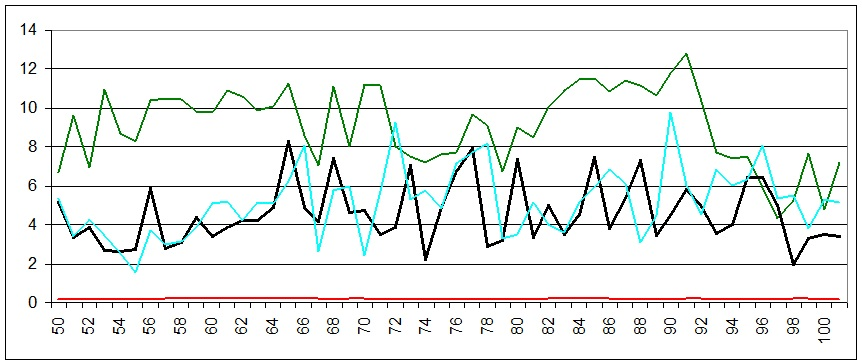
\includegraphics[width=0.8\textwidth]{sperimentazioni/united/Grafici/Ahead1/1.jpg}
\caption{dewp ahead 1}
\label{1A1}
}
\end{figure}

\medskip

Ahead = 2 

\begin{figure}[H]
\textbf{
\centering
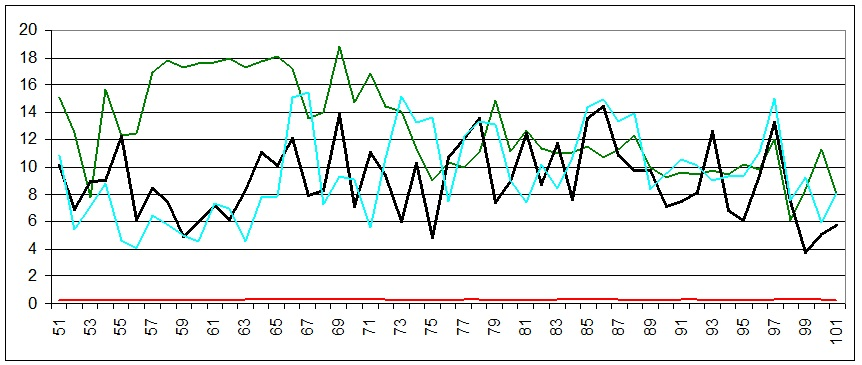
\includegraphics[width=0.8\textwidth]{sperimentazioni/united/Grafici/Ahead2/1.jpg}
\caption{dewp ahead 2}
\label{1A2}
}
\end{figure}

\newpage

Ahead = 3

\begin{figure}[H]
\textbf{
\centering
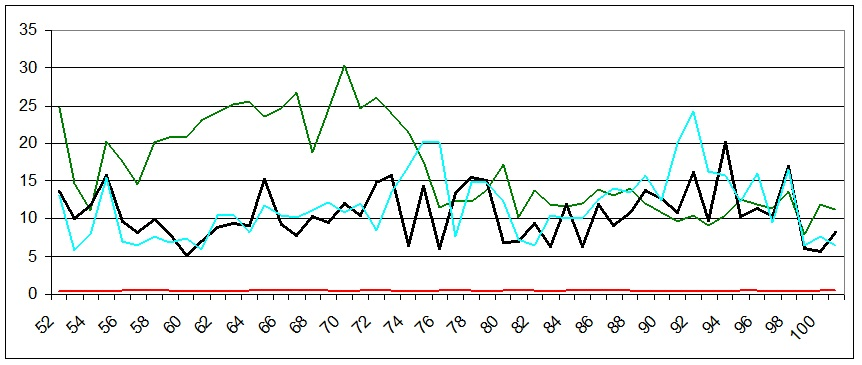
\includegraphics[width=0.8\textwidth]{sperimentazioni/united/Grafici/Ahead3/1.jpg}
\caption{dewp ahead 3}
\label{1A3}
}
\end{figure}

Ahead = 4 

\begin{figure}[H]
\textbf{
\centering
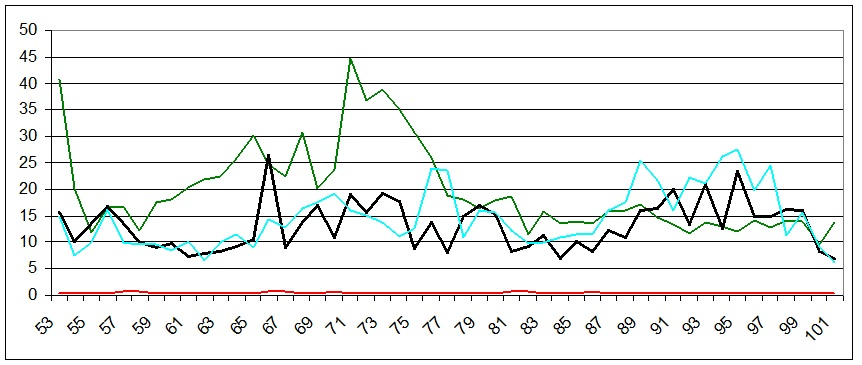
\includegraphics[width=0.8\textwidth]{sperimentazioni/united/Grafici/Ahead4/1.jpg}
\caption{dewp ahead 4}
\label{1A4}
}
\end{figure}

Ahead = 5

\begin{figure}[H]
\textbf{
\centering
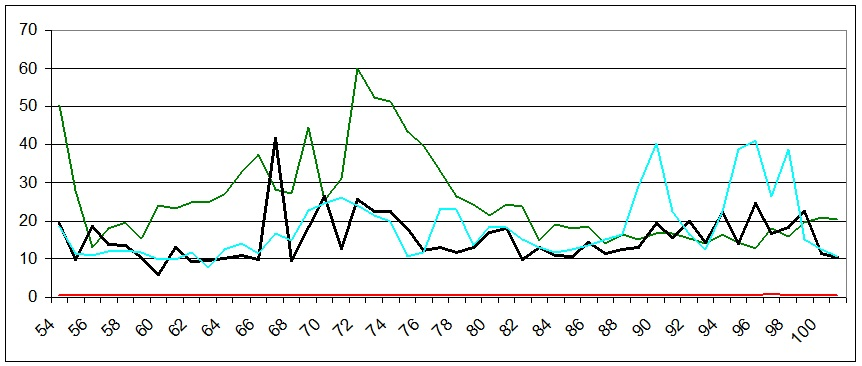
\includegraphics[width=0.8\textwidth]{sperimentazioni/united/Grafici/Ahead5/1.jpg}
\caption{dewp ahead 5}
\label{1A5}
}
\end{figure}

Ahead = 6 

\begin{figure}[H]
\textbf{
\centering
\includegraphics[width=0.8\textwidth]{sperimentazioni/united/Grafici/Ahead6/1.jpg}
\caption{dewp ahead 6}
\label{1A6}
}
\end{figure}

\textbf{Attributo: pres}

\medskip

Ahead = 1

\begin{figure}[H]
\textbf{
\centering
\includegraphics[width=0.8\textwidth]{sperimentazioni/united/Grafici/Ahead1/2.jpg}
\caption{pres ahead 1}
\label{2A1}
}
\end{figure}

Ahead = 2 

\begin{figure}[H]
\textbf{
\centering
\includegraphics[width=0.8\textwidth]{sperimentazioni/united/Grafici/Ahead2/2.jpg}
\caption{pres ahead 2}
\label{2A2}
}
\end{figure}

Ahead = 3

\begin{figure}[H]
\textbf{
\centering
\includegraphics[width=0.8\textwidth]{sperimentazioni/united/Grafici/Ahead3/2.jpg}
\caption{pres ahead 3}
\label{2A3}
}
\end{figure}

Ahead = 4 

\begin{figure}[H]
\textbf{
\centering
\includegraphics[width=0.8\textwidth]{sperimentazioni/united/Grafici/Ahead4/2.jpg}
\caption{pres ahead 4}
\label{2A4}
}
\end{figure}

Ahead = 5

\begin{figure}[H]
\textbf{
\centering
\includegraphics[width=0.8\textwidth]{sperimentazioni/united/Grafici/Ahead5/2.jpg}
\caption{pres ahead 5}
\label{2A5}
}
\end{figure}

Ahead = 6 

\begin{figure}[H]
\textbf{
\centering
\includegraphics[width=0.8\textwidth]{sperimentazioni/united/Grafici/Ahead6/2.jpg}
\caption{pres ahead 6}
\label{2A6}
}
\end{figure}

\textbf{Attributo: temp}

Ahead = 1

\begin{figure}[H]
\textbf{
\centering
\includegraphics[width=0.8\textwidth]{sperimentazioni/united/Grafici/Ahead1/3.jpg}
\caption{temp ahead 1}
\label{3A1}
}
\end{figure}

Ahead = 2 

\begin{figure}[H]
\textbf{
\centering
\includegraphics[width=0.8\textwidth]{sperimentazioni/united/Grafici/Ahead2/3.jpg}
\caption{temp ahead 2}
\label{3A2}
}
\end{figure}

Ahead = 3

\begin{figure}[H]
\textbf{
\centering
\includegraphics[width=0.8\textwidth]{sperimentazioni/united/Grafici/Ahead3/3.jpg}
\caption{temp ahead 3}
\label{3A3}
}
\end{figure}

Ahead = 4 

\begin{figure}[H]
\textbf{
\centering
\includegraphics[width=0.8\textwidth]{sperimentazioni/united/Grafici/Ahead4/3.jpg}
\caption{temp ahead 4}
\label{3A4}
}
\end{figure}

Ahead = 5

\begin{figure}[H]
\textbf{
\centering
\includegraphics[width=0.8\textwidth]{sperimentazioni/united/Grafici/Ahead5/3.jpg}
\caption{temp ahead 5}
\label{3A5}
}
\end{figure}

Ahead = 6 

\begin{figure}[H]
\textbf{
\centering
\includegraphics[width=0.8\textwidth]{sperimentazioni/united/Grafici/Ahead6/3.jpg}
\caption{temp ahead 6}
\label{3A6}
}
\end{figure}

\textbf{Attributo: wind}

Ahead = 1

\begin{figure}[H]
\textbf{
\centering
\includegraphics[width=0.8\textwidth]{sperimentazioni/united/Grafici/Ahead1/4.jpg}
\caption{wind ahead 1}
\label{4A1}
}
\end{figure}

Ahead = 2 

\begin{figure}[H]
\textbf{
\centering
\includegraphics[width=0.8\textwidth]{sperimentazioni/united/Grafici/Ahead2/4.jpg}
\caption{wind ahead 2}
\label{4A2}
}
\end{figure}

Ahead = 3

\begin{figure}[H]
\textbf{
\centering
\includegraphics[width=0.8\textwidth]{sperimentazioni/united/Grafici/Ahead3/4.jpg}
\caption{wind ahead 3}
\label{4A3}
}
\end{figure}

Ahead = 4 

\begin{figure}[H]
\textbf{
\centering
\includegraphics[width=0.8\textwidth]{sperimentazioni/united/Grafici/Ahead4/4.jpg}
\caption{wind ahead 4}
\label{4A4}
}
\end{figure}

Ahead = 5

\begin{figure}[H]
\textbf{
\centering
\includegraphics[width=0.8\textwidth]{sperimentazioni/united/Grafici/Ahead5/4.jpg}
\caption{wind ahead 5}
\label{4A5}
}
\end{figure}

Ahead = 6 

\begin{figure}[H]
\textbf{
\centering
\includegraphics[width=0.8\textwidth]{sperimentazioni/united/Grafici/Ahead6/4.jpg}
\caption{wind ahead 6}
\label{4A6}
}
\end{figure}


A differenza del dataset Ecotexas, in UnitedStatesPacific, le versioni VARForecaster 2.1 e VARForecaster 2.2, come è possibile vedere da Fig.~\ref{1A1} a Fig.~\ref{4A6}, apportano delle migliorie alle previsioni effettuate dalla versione VARForecaster 2.0.

La versione VARForecaster 1.0 invece, è nettamente più accurata.

Valutando invece l'efficienza, si nota, dalla Tab. 4.132 alla Tab. 4.134, che il versione VARForecaster 2.2 è quella con il costo computazione in tempo minore.

\chapter{Conclusioni}
Questo lavoro di tesi, come descritto nel cap. 1, mira a ridurre il trade-off tra accuratezza ed efficienza presentato nelle versioni del software VARForecaster in \cite{donato}. Per cercare di raggiungere questo obiettivo è stato deciso di:
\begin{itemize}
\item modificare il modo in cui viene calcolato l'aggregato associato ad ogni cluster, nel momento in esso viene creato nella fase di ri-apprendimento del \textit{CT}. Infatti si è passato dal copiare l'aggregato dal cluster padre, quindi dando un forte peso alle rilevazioni effettuate dai sensori che ricadevano nel cluster negli istanti precedenti a \textit{t}, al calcolare tale oggetto attraverso l'utilizzo delle funzioni di media o di mediana, a discrezione dell'utente, e di conseguenza far si che l'aggregato rispecchi i valori presenti all'interno delle serie temporali dei sensori attualmente ricadenti nel cluster;
\item applicare una funzione di smoothing esponenziale, nello specifico il \textit{metodo di Bolt}, a diversi livelli di $\alpha$. Si è provato infatti a dare maggior peso alle precedenti rilevazioni di \textit{t}, associando ad esse un peso specifico maggiore, ad assegnare lo stesso peso alle rilevazioni precedenti a \textit{t} e ai valori rilevati in \textit{t}, oppure a valorizzare maggiormente le rilevazioni di \textit{t} a discapito delle precedenti.
\end{itemize}

La struttura di questo progetto di tesi è modulata in modo tale da fornire gli strumenti storici e tecnici delle principali tecniche utilizzate al suo interno, nel cap. 2, cosicché da permettere una più facile comprensione degli algoritmi sviluppati in esso, descritti invece nel cap. 3. 

I risultati delle sperimentazioni effettuate, mostrate nel cap. 4, provano che le versioni VARForecaster 2.1 e VARForecaster 2.2 sono quasi sempre più accurate della versione VARForecaster 2.0, a discapito di una minima perdita in tempi di costi computazionali, comunque del tutto sostenibili (si è nell'ordine di pochissimi millisecondi per snapshot).

Per quello che riguarda invece la versione VARForecaster 1.0, la scelta è strettamente legata ai fenomeni rilevati all'interno del dataset. 

Un dataset poco regolare, come lo è Ecotexas, permette indistintamente l'utilizzo delle versioni VARForecaster 1.0, VARForecaster 2.1 e VARForecaster 2.2, dando la possibilità di avere un indiscusso guadagno in termini di costi computazionali in tempo nel caso si scegliesse una versione tra VARForecaster 2.1 e VARForecaster 2.2. 

Un dataset più regolare nelle rilevazioni, invece, come per esempio UnitedStatesPacific, mette di fronte ad una drastica differenza di accuratezza tra le versioni VARForecaster 1.0, VARForecaster 2.1 e VARForecaster 2.2, facendo preferire tra tutte la prima. 

\medskip

Eventuali sviluppi futuri potrebbero prevedere un'ibridazione tra i sistemi VARForecaster 2.1-VARForecaster 2.2 e il sistema VARForecaster 1.0, andando a creare da zero, ad ogni snapshot, un nuovo \textit{CT}.

Questo potrebbe essere utile al fine di avere un \textit{CT} creato ad-hoc per i dati realmente rilevati ad ogni snapshot, avendo comunque un aumento dell'efficienza a minor discapito dell'accuratezza. 
\chapter{Appendice}
\section{Guida per l’esecuzione di VARForecaster 2.1/2.2}

Per poter eseguire VARForecaster 2.1/2.2 è necessario che siano installati sia Java che il software R, e per quest'ultimo che siano scaricati i pacchetti descritti nel par. 2.2.

Per avviare l'eseguibile, basta aprire il \textit{prompt dei comandi} e spostarsi nella cartella ove è posizionato il .jar (in seguito \textit{root}).

Bisogna poi inserire dei parametri che indicano alcuni valori indispensabili all'esecuzione degli stessi. I parametri da inserire nel caso in cui si volesse eseguire VARForecaster 2.1 sono differenti da quelli che richiede la versione VARForecaster 2.2, ma entrambe richiedono una gerarchia di cartelle ben definita. 

Per l'esattezza ci devono essere, nella root:
\begin{itemize}
\item \textbf{root}
\begin{itemize}
\item R
\begin{itemize}
\item Parameters
\item RMSE
\end{itemize}
\item stream
\begin{itemize}
\item forecast
\item model
\item report
\begin{itemize}
\item clustering
\item ComputationTime
\item ForecastRMSE
\end{itemize}
\item smoothing [necessaria solo nella versione VARForecaster 2.2]
\item weight
\end{itemize}
\end{itemize}
\item dataset
\end{itemize}

\section*{Parametri VARForecaster 2.1}
A seguito della dicitura, nel prompt dei comandi \textit{"java -jar VARForecasterv1"} (dove VARForecasterv1 è il file eseguibile della versione VARForecaster 2.1), è necessario inserire i seguenti parametri:
\begin{itemize}
\item argomento 0: nome del file .arff (senza estensione);
\item argomento 1: nome del file .ini (senza estensione);
\item argomento 2: numero massimo di split da effettuare;
\item argomento 3: valore di bperc.;
\item argomento 4: dimensione della finestra temporale (dim);
\item argomento 5: percorso dello script R;
\item argomento 6: valore del lag.max (parametro necessario alla costruzione del modello VAR). Può valere al massimo \textit{dim-2};
\item argomento 7: valore di season. Nel caso in cui non ci fosse stagionalità è possibile inserire il valore "NULL";
\item argomento 8: matrici delle variabili esogene. È possibile inserire il valore "NULL" nel caso in cui non ci fossero variabili esogene.;
\item argomento 9: valore di \textit{ic} (parametro necessario alla costruzione del modello VAR);
\item argomento 10: valore di \textit{type} (parametro necessario alla costruzione del modello VAR);
\item argomento 11: numero di istanti per cui fare predizione;
\item argomento 12: percorso completo della \textit{root}, seguito dal carattere $\textbackslash$ ;
\item argomento 13: parametro per la scelta della modalità di calcolo dell'aggregato. Inserire "median" se si intende calcolarlo tramite mediana, o "avg" se si vuole farlo utilizzando la media.
\item argomento 14: parametro che indica se utilizzare l'indice di autocorrelazione spaziale Getis and Ord oppure la varianza. Inserire "true" per utilizzare il Getis and Ord, in alternativa "false" per la varianza.
\end{itemize}
\section*{Parametri VARForecaster 2.2}
Per la versione VARForecaster 2.2, oltre che il comando \textit{java -jar VARForecasterv2} (dove VARForecasterv2 è l'eseguibile per la versione VARForecaster 2.2) è necessario specificare i seguenti parametri:
\begin{itemize}
\item argomento 0: nome del file .arff (senza estensione);
\item argomento 1: nome del file .ini (senza estensione);
\item argomento 2: numero massimo di split da effettuare;
\item argomento 3: valore di bperc.;
\item argomento 4: dimensione della finestra temporale (dim);
\item argomento 5: percorso dello script R;
\item argomento 6: valore del lag.max (parametro necessario alla costruzione del modello VAR). Può valere al massimo \textit{dim-2};
\item argomento 7: valore di season. Nel caso in cui non ci fosse stagionalità è possibile inserire il valore "NULL";
\item argomento 8: matrici delle variabili esogene. È possibile inserire il valore "NULL" nel caso in cui non ci fossero variabili esogene.;
\item argomento 9: valore di \textit{ic} (parametro necessario alla costruzione del modello VAR);
\item argomento 10: valore di \textit{type} (parametro necessario alla costruzione del modello VAR);
\item argomento 11: numero di istanti per cui fare predizione;
\item argomento 12: percorso completo della \textit{root}, seguito dal carattere $\textbackslash$ ;
\item argomento 13: parametro per la scelta della modalità di calcolo dell'aggregato. Inserire "median" se si intende calcolarlo tramite mediana, o "avg" se si vuole farlo utilizzando la media.
\item argomento 14: valore del livello $\alpha$ ( 0 $\leq$ $\alpha$ $\leq$ 1);
\item argomento 15: parametro che indica se utilizzare l'indice di autocorrelazione spaziale Getis and Ord oppure la varianza. Inserire "true" per utilizzare il Getis and Ord, in alternativa "false" per la varianza.
\end{itemize}
  \begin{thebibliography}{1}
 \addcontentsline{toc}{chapter}{Bibliografia}
  \bibitem{donato} D. Mastropasqua. {\em Apprendimento di cluster spazio-temporali per l'apprendimento di un modello VAR}, 2016: Tesi di laurea in Algoritmi e Strutture Dati, Uniba.

  \bibitem{2a} G. Data, P. Mariani. {\em Market Access nel settore healthcare – Strategie, attori, attività e processi}, 2015:  FrancoAngeli Editori.

  \bibitem{3a} C. Alexander. {\em Market Risk Analysis, Value at Risk Models}, 2009: Wiley.

  \bibitem{4a} N. Fanizzi. {\em Corso di Apprendimento Automatico}, 2009: Laurea Magistrale in Informatica, Uniba.
  
  \bibitem{5a} H. Arsham. {\em Forecasting by Smoothing Techniques}, 2015.
  
  \bibitem{6a} M. Brett. {\em Corso di Apprendimento Automatico}, 2013 : MRC Cognition and Brain Sciences Unit.
  
    \bibitem{7a} R.J. Hyndman, G. Athanasopoulos. {\em Forecasting: principles and practice}, 2013.
    
    \bibitem{8a} G. Righini. {\em Corso di Logistica}, 2013: Laurea Magistrale in Informatica, Unimi.
    \bibitem{9a} C.A. Sims. {\em Macroeconomics and Reality}, 1980.
    
    \bibitem{10a} J.D. Hamilton. {\em Time Series Analysis}, 1994: Princeton University Press.
   
    \bibitem{11a} D. Buono. {\em Analisi econometrica dinamica del settore Agricoltura}, 2007: Tesi di dottorato in Scienze Economiche, Unina.
    
    \bibitem{12a} {\em https://www.r-project.org/about.html}.
    
    \bibitem{13a} V. Fanelli. {\em Uso di modelli VAR nella previsione di modelli di regressione in una rete di sensori multi-variati}, 2015: Tesi di laurea in Metodi Avanzati di Programmazione, Uniba.
    
     \bibitem{14a} {\em https://it.wikipedia.org/wiki/Outlier}.
     
     \bibitem{15a} M. Ross Sheldon. {\em Introduzione alla statistica}, 2014, Maggioli Editore.
      
     \bibitem{16a} L. Bing. {\em Web Data Mining Exploring Hyperlinks, Contents, and Usage Data}, 2011, par. 4.1.
     
     \bibitem{17a} L. Bing. {\em Web Data Mining Exploring Hyperlinks, Contents, and Usage Data}, 2011, par. 4.2.
     
     \bibitem{18a} L. Bing. {\em Web Data Mining Exploring Hyperlinks, Contents, and Usage Data}, 2011, par. 4.3.
     
      \bibitem{19a} A. Appice, D. Malerba {\em Leveraging the power of local spatial autocorrelation in geophysical interpolative clustering, Data Mining and Knowledge Discovery}, 2014, cap. 2.
          
     \bibitem{20a} {\em https://cran.r-project.org/web/packages/vars/vars.pdf}.
      
  \end{thebibliography}
\chapter*{Ringraziamenti}



\end{document}